\documentclass[a4paper]{book}
\usepackage{makeidx}
\usepackage{natbib}
\usepackage{graphicx}
\usepackage{multicol}
\usepackage{float}
\usepackage{listings}
\usepackage{color}
\usepackage{ifthen}
\usepackage[table]{xcolor}
\usepackage{textcomp}
\usepackage{alltt}
\usepackage{ifpdf}
\ifpdf
\usepackage[pdftex,
            pagebackref=true,
            colorlinks=true,
            linkcolor=blue,
            unicode
           ]{hyperref}
\else
\usepackage[ps2pdf,
            pagebackref=true,
            colorlinks=true,
            linkcolor=blue,
            unicode
           ]{hyperref}
\usepackage{pspicture}
\fi
\usepackage[utf8]{inputenc}
\usepackage{mathptmx}
\usepackage[scaled=.90]{helvet}
\usepackage{courier}
\usepackage{sectsty}
\usepackage[titles]{tocloft}
\usepackage{doxygen}
\lstset{language=C++,inputencoding=utf8,basicstyle=\footnotesize,breaklines=true,breakatwhitespace=true,tabsize=8,numbers=left }
\makeindex
\setcounter{tocdepth}{3}
\renewcommand{\footrulewidth}{0.4pt}
\renewcommand{\familydefault}{\sfdefault}
\hfuzz=15pt
\setlength{\emergencystretch}{15pt}
\hbadness=750
\tolerance=750
\begin{document}
\hypersetup{pageanchor=false,citecolor=blue}
\begin{titlepage}
\vspace*{7cm}
\begin{center}
{\Large \-My \-Project }\\
\vspace*{1cm}
{\large \-Generated by Doxygen 1.7.6.1}\\
\vspace*{0.5cm}
{\small Sun Apr 27 2014 14:13:02}\\
\end{center}
\end{titlepage}
\clearemptydoublepage
\pagenumbering{roman}
\tableofcontents
\clearemptydoublepage
\pagenumbering{arabic}
\hypersetup{pageanchor=true,citecolor=blue}
\chapter{\-Class \-Index}
\section{\-Class \-Hierarchy}
\-This inheritance list is sorted roughly, but not completely, alphabetically\-:\begin{DoxyCompactList}
\item \contentsline{section}{\-Arc\-\_\-t}{\pageref{structArc__t}}{}
\item \contentsline{section}{asfig}{\pageref{structasfig}}{}
\item \contentsline{section}{asisc}{\pageref{structasisc}}{}
\item \contentsline{section}{asiss}{\pageref{structasiss}}{}
\item \contentsline{section}{asobj}{\pageref{structasobj}}{}
\item \contentsline{section}{asosc}{\pageref{structasosc}}{}
\item \contentsline{section}{\-Basic\-\_\-block}{\pageref{classBasic__block}}{}
\item \contentsline{section}{\-Cfg}{\pageref{classCfg}}{}
\item \contentsline{section}{dep}{\pageref{structdep}}{}
\item \contentsline{section}{\-Dfg}{\pageref{classDfg}}{}
\item \contentsline{section}{\-Function}{\pageref{classFunction}}{}
\item \contentsline{section}{\-Line}{\pageref{classLine}}{}
\begin{DoxyCompactList}
\item \contentsline{section}{\-Directive}{\pageref{classDirective}}{}
\item \contentsline{section}{\-Instruction}{\pageref{classInstruction}}{}
\item \contentsline{section}{\-Label}{\pageref{classLabel}}{}
\end{DoxyCompactList}
\item \contentsline{section}{\-Node}{\pageref{classNode}}{}
\item \contentsline{section}{\-Node\-\_\-dfg}{\pageref{classNode__dfg}}{}
\item \contentsline{section}{\-Operand}{\pageref{classOperand}}{}
\begin{DoxyCompactList}
\item \contentsline{section}{\-O\-P\-Expression}{\pageref{classOPExpression}}{}
\item \contentsline{section}{\-O\-P\-Immediate}{\pageref{classOPImmediate}}{}
\item \contentsline{section}{\-O\-P\-Label}{\pageref{classOPLabel}}{}
\item \contentsline{section}{\-O\-P\-Register}{\pageref{classOPRegister}}{}
\end{DoxyCompactList}
\item \contentsline{section}{\-Program}{\pageref{classProgram}}{}
\item \contentsline{section}{s\-\_\-\-Profile}{\pageref{structs__Profile}}{}
\item \contentsline{section}{\-Test\-O\-P\-Label}{\pageref{classTestOPLabel}}{}
\item \contentsline{section}{utchn}{\pageref{structutchn}}{}
\item \contentsline{section}{utdat}{\pageref{unionutdat}}{}
\item \contentsline{section}{utdic}{\pageref{structutdic}}{}
\item \contentsline{section}{utdit}{\pageref{structutdit}}{}
\item \contentsline{section}{uttdc}{\pageref{structuttdc}}{}
\item \contentsline{section}{uttpd}{\pageref{structuttpd}}{}
\item \contentsline{section}{uttyp}{\pageref{structuttyp}}{}
\item \contentsline{section}{\-Y\-Y\-S\-T\-Y\-P\-E}{\pageref{unionYYSTYPE}}{}
\end{DoxyCompactList}

\chapter{\-Class \-Index}
\section{\-Class \-List}
\-Here are the classes, structs, unions and interfaces with brief descriptions\-:\begin{DoxyCompactList}
\item\contentsline{section}{\hyperlink{structArc__t}{\-Arc\-\_\-t} }{\pageref{structArc__t}}{}
\item\contentsline{section}{\hyperlink{structasfig}{asfig} }{\pageref{structasfig}}{}
\item\contentsline{section}{\hyperlink{structasisc}{asisc} }{\pageref{structasisc}}{}
\item\contentsline{section}{\hyperlink{structasiss}{asiss} }{\pageref{structasiss}}{}
\item\contentsline{section}{\hyperlink{structasobj}{asobj} }{\pageref{structasobj}}{}
\item\contentsline{section}{\hyperlink{structasosc}{asosc} }{\pageref{structasosc}}{}
\item\contentsline{section}{\hyperlink{classBasic__block}{\-Basic\-\_\-block} \\*\-Class representing a \hyperlink{classBasic__block}{\-Basic\-\_\-block} of a fonction }{\pageref{classBasic__block}}{}
\item\contentsline{section}{\hyperlink{classCfg}{\-Cfg} \\*\-Class representing control flow graph }{\pageref{classCfg}}{}
\item\contentsline{section}{\hyperlink{structdep}{dep} }{\pageref{structdep}}{}
\item\contentsline{section}{\hyperlink{classDfg}{\-Dfg} \\*\-Class representing a \hyperlink{classDfg}{\-Dfg} of a \-Basic block, a data flow graph that is to be used to calculate the critical path and schedule code }{\pageref{classDfg}}{}
\item\contentsline{section}{\hyperlink{classDirective}{\-Directive} \\*\-Class representing an \hyperlink{classDirective}{\-Directive} herited by \hyperlink{classLine}{\-Line} }{\pageref{classDirective}}{}
\item\contentsline{section}{\hyperlink{classFunction}{\-Function} \\*\-Class representing a \hyperlink{classFunction}{\-Function} on a program }{\pageref{classFunction}}{}
\item\contentsline{section}{\hyperlink{classInstruction}{\-Instruction} \\*\-Class representing an instruction which herited by \hyperlink{classLine}{\-Line} }{\pageref{classInstruction}}{}
\item\contentsline{section}{\hyperlink{classLabel}{\-Label} \\*\-Class representing an \hyperlink{classLabel}{\-Label} herited by \hyperlink{classLine}{\-Line} }{\pageref{classLabel}}{}
\item\contentsline{section}{\hyperlink{classLine}{\-Line} \\*\-Abstract class representing an \hyperlink{classLine}{\-Line} }{\pageref{classLine}}{}
\item\contentsline{section}{\hyperlink{classNode}{\-Node} \\*\-Class representing a \hyperlink{classNode}{\-Node} in list }{\pageref{classNode}}{}
\item\contentsline{section}{\hyperlink{classNode__dfg}{\-Node\-\_\-dfg} \\*\-Class representing a node of data flow graph }{\pageref{classNode__dfg}}{}
\item\contentsline{section}{\hyperlink{classOperand}{\-Operand} \\*\-Abstract class representing an operand }{\pageref{classOperand}}{}
\item\contentsline{section}{\hyperlink{classOPExpression}{\-O\-P\-Expression} \\*\-Class representing an expression herited by \hyperlink{classOperand}{\-Operand} }{\pageref{classOPExpression}}{}
\item\contentsline{section}{\hyperlink{classOPImmediate}{\-O\-P\-Immediate} \\*\-Class representing an \-Immediate herited by \hyperlink{classOperand}{\-Operand} }{\pageref{classOPImmediate}}{}
\item\contentsline{section}{\hyperlink{classOPLabel}{\-O\-P\-Label} \\*\-Class representing a \hyperlink{classLabel}{\-Label} herited by \hyperlink{classOperand}{\-Operand} }{\pageref{classOPLabel}}{}
\item\contentsline{section}{\hyperlink{classOPRegister}{\-O\-P\-Register} \\*\-Class representing a \-Register herited by \hyperlink{classOperand}{\-Operand} }{\pageref{classOPRegister}}{}
\item\contentsline{section}{\hyperlink{classProgram}{\-Program} \\*\-Class representing a program as list of lines }{\pageref{classProgram}}{}
\item\contentsline{section}{\hyperlink{structs__Profile}{s\-\_\-\-Profile} \\*\-Structure allowing to add caracteristics to an operator }{\pageref{structs__Profile}}{}
\item\contentsline{section}{\hyperlink{classTestOPLabel}{\-Test\-O\-P\-Label} }{\pageref{classTestOPLabel}}{}
\item\contentsline{section}{\hyperlink{structutchn}{utchn} }{\pageref{structutchn}}{}
\item\contentsline{section}{\hyperlink{unionutdat}{utdat} }{\pageref{unionutdat}}{}
\item\contentsline{section}{\hyperlink{structutdic}{utdic} }{\pageref{structutdic}}{}
\item\contentsline{section}{\hyperlink{structutdit}{utdit} }{\pageref{structutdit}}{}
\item\contentsline{section}{\hyperlink{structuttdc}{uttdc} }{\pageref{structuttdc}}{}
\item\contentsline{section}{\hyperlink{structuttpd}{uttpd} }{\pageref{structuttpd}}{}
\item\contentsline{section}{\hyperlink{structuttyp}{uttyp} }{\pageref{structuttyp}}{}
\item\contentsline{section}{\hyperlink{unionYYSTYPE}{\-Y\-Y\-S\-T\-Y\-P\-E} }{\pageref{unionYYSTYPE}}{}
\end{DoxyCompactList}

\chapter{\-File \-Index}
\section{File List}
Here is a list of all documented files with brief descriptions\-:\begin{DoxyCompactList}
\item\contentsline{section}{{\bfseries asm200.\-h} }{\pageref{asm200_8h}}{}
\item\contentsline{section}{{\bfseries asm\-\_\-mipsyac.\-h} }{\pageref{asm__mipsyac_8h}}{}
\item\contentsline{section}{\hyperlink{_basic__block_8h}{Basic\-\_\-block.\-h} \\*\hyperlink{class_basic__block}{Basic\-\_\-block} class }{\pageref{_basic__block_8h}}{}
\item\contentsline{section}{\hyperlink{_cfg_8h}{Cfg.\-h} \\*\hyperlink{class_cfg}{Cfg} class }{\pageref{_cfg_8h}}{}
\item\contentsline{section}{\hyperlink{_dfg_8h}{Dfg.\-h} \\*\hyperlink{class_dfg}{Dfg} class }{\pageref{_dfg_8h}}{}
\item\contentsline{section}{\hyperlink{_directive_8h}{Directive.\-h} \\*\hyperlink{class_directive}{Directive} class }{\pageref{_directive_8h}}{}
\item\contentsline{section}{{\bfseries Enum\-\_\-type.\-h} }{\pageref{_enum__type_8h}}{}
\item\contentsline{section}{\hyperlink{_function_8h}{Function.\-h} \\*\hyperlink{class_function}{Function} class }{\pageref{_function_8h}}{}
\item\contentsline{section}{\hyperlink{_instruction_8h}{Instruction.\-h} \\*\hyperlink{class_instruction}{Instruction} class }{\pageref{_instruction_8h}}{}
\item\contentsline{section}{\hyperlink{_label_8h}{Label.\-h} \\*\hyperlink{class_label}{Label} class }{\pageref{_label_8h}}{}
\item\contentsline{section}{\hyperlink{_line_8h}{Line.\-h} \\*\hyperlink{class_line}{Line} class }{\pageref{_line_8h}}{}
\item\contentsline{section}{\hyperlink{_node_8h}{Node.\-h} \\*\hyperlink{class_node}{Node} class }{\pageref{_node_8h}}{}
\item\contentsline{section}{\hyperlink{_node__dfg_8h}{Node\-\_\-dfg.\-h} \\*\hyperlink{class_node__dfg}{Node\-\_\-dfg} class }{\pageref{_node__dfg_8h}}{}
\item\contentsline{section}{\hyperlink{_operand_8h}{Operand.\-h} \\*\hyperlink{class_operand}{Operand} class }{\pageref{_operand_8h}}{}
\item\contentsline{section}{\hyperlink{_o_p_expression_8h}{O\-P\-Expression.\-h} \\*\hyperlink{class_o_p_expression}{O\-P\-Expression} class }{\pageref{_o_p_expression_8h}}{}
\item\contentsline{section}{\hyperlink{_o_p_immediate_8h}{O\-P\-Immediate.\-h} \\*\hyperlink{class_o_p_immediate}{O\-P\-Immediate} class }{\pageref{_o_p_immediate_8h}}{}
\item\contentsline{section}{\hyperlink{_o_p_label_8h}{O\-P\-Label.\-h} \\*\hyperlink{class_o_p_label}{O\-P\-Label} class }{\pageref{_o_p_label_8h}}{}
\item\contentsline{section}{\hyperlink{_o_p_register_8h}{O\-P\-Register.\-h} \\*\hyperlink{class_o_p_register}{O\-P\-Register} class }{\pageref{_o_p_register_8h}}{}
\item\contentsline{section}{\hyperlink{_program_8h}{Program.\-h} \\*\hyperlink{class_program}{Program} class }{\pageref{_program_8h}}{}
\item\contentsline{section}{{\bfseries Test\-O\-P\-Label.\-h} }{\pageref{_test_o_p_label_8h}}{}
\item\contentsline{section}{{\bfseries utl200.\-h} }{\pageref{utl200_8h}}{}
\end{DoxyCompactList}

\chapter{\-Class \-Documentation}
\hypertarget{structArc__t}{\section{\-Arc\-\_\-t \-Struct \-Reference}
\label{structArc__t}\index{\-Arc\-\_\-t@{\-Arc\-\_\-t}}
}
\subsection*{\-Public \-Attributes}
\begin{DoxyCompactItemize}
\item 
\hypertarget{structArc__t_a629d4a4e9c44aae452c7d54979c82abe}{int {\bfseries delai}}\label{structArc__t_a629d4a4e9c44aae452c7d54979c82abe}

\item 
\hypertarget{structArc__t_a75234bf2ed3084da0bf5b8fbc52fdc67}{t\-\_\-\-Dep {\bfseries dep}}\label{structArc__t_a75234bf2ed3084da0bf5b8fbc52fdc67}

\item 
\hypertarget{structArc__t_af7eaf6285792517ed5f06eba6abe3211}{\hyperlink{classNode__dfg}{\-Node\-\_\-dfg} $\ast$ {\bfseries next}}\label{structArc__t_af7eaf6285792517ed5f06eba6abe3211}

\end{DoxyCompactItemize}


\-The documentation for this struct was generated from the following file\-:\begin{DoxyCompactItemize}
\item 
\hyperlink{Node__dfg_8h}{\-Node\-\_\-dfg.\-h}\end{DoxyCompactItemize}

\hypertarget{structasfig}{\section{asfig Struct Reference}
\label{structasfig}\index{asfig@{asfig}}
}
\subsection*{Public Attributes}
\begin{DoxyCompactItemize}
\item 
\hypertarget{structasfig_acb2f83dbe7a1e3cc29529820c2d84f08}{struct \hyperlink{structutdic}{utdic} $\ast$ {\bfseries G\-L\-B\-\_\-\-D\-I\-C}}\label{structasfig_acb2f83dbe7a1e3cc29529820c2d84f08}

\item 
\hypertarget{structasfig_a0d08a06c7ef0d7d128b068e63ec65a08}{struct \hyperlink{structuttyp}{uttyp} $\ast$ {\bfseries G\-L\-B\-\_\-\-S\-Y\-M}}\label{structasfig_a0d08a06c7ef0d7d128b068e63ec65a08}

\item 
\hypertarget{structasfig_ae87202e68aa58ff7cf9d39b476d81d13}{struct \hyperlink{structuttyp}{uttyp} $\ast$ {\bfseries M\-E\-M\-\_\-\-T\-A\-B}}\label{structasfig_ae87202e68aa58ff7cf9d39b476d81d13}

\item 
\hypertarget{structasfig_a29babddc26cd0b8fec9c3c139dd78206}{struct \hyperlink{structasosc}{asosc} $\ast$ {\bfseries O\-U\-T\-\_\-\-S\-E\-C}}\label{structasfig_a29babddc26cd0b8fec9c3c139dd78206}

\item 
\hypertarget{structasfig_acdd790bc6a90c1a53d9c96d651d515ae}{struct \hyperlink{structasisc}{asisc} $\ast$ {\bfseries I\-N\-\_\-\-S\-E\-C}}\label{structasfig_acdd790bc6a90c1a53d9c96d651d515ae}

\item 
\hypertarget{structasfig_a7811bcfbf0a2fd6c47b0f457875d1379}{struct \hyperlink{structasobj}{asobj} $\ast$ {\bfseries O\-B\-J\-E\-C\-T\-S}}\label{structasfig_a7811bcfbf0a2fd6c47b0f457875d1379}

\item 
\hypertarget{structasfig_aef8acd1ebd4a06c7be326a16a3d587fc}{unsigned int {\bfseries F\-L\-A\-G}}\label{structasfig_aef8acd1ebd4a06c7be326a16a3d587fc}

\end{DoxyCompactItemize}


The documentation for this struct was generated from the following file\-:\begin{DoxyCompactItemize}
\item 
asm200.\-h\end{DoxyCompactItemize}

\hypertarget{structasisc}{\section{asisc Struct Reference}
\label{structasisc}\index{asisc@{asisc}}
}
\subsection*{Public Attributes}
\begin{DoxyCompactItemize}
\item 
\hypertarget{structasisc_ad9e1171351b4def0dee34a931bef06c2}{struct \hyperlink{structasisc}{asisc} $\ast$ {\bfseries N\-E\-X\-T}}\label{structasisc_ad9e1171351b4def0dee34a931bef06c2}

\item 
\hypertarget{structasisc_a556fa34f54b5c9c75dd76650538afc1d}{char $\ast$ {\bfseries I\-D\-E\-N\-T}}\label{structasisc_a556fa34f54b5c9c75dd76650538afc1d}

\item 
\hypertarget{structasisc_a719068c36a0e9705bf73ee2f073c423d}{struct \hyperlink{structasosc}{asosc} $\ast$ {\bfseries O\-U\-T\-\_\-\-S\-E\-C}}\label{structasisc_a719068c36a0e9705bf73ee2f073c423d}

\item 
\hypertarget{structasisc_a2d489dd1bf43e16f31806a7e22b4c944}{unsigned int {\bfseries P\-O\-S\-I\-T\-I\-O\-N}}\label{structasisc_a2d489dd1bf43e16f31806a7e22b4c944}

\item 
\hypertarget{structasisc_acbc421dc86cceaf4736c520ab2380d76}{unsigned int {\bfseries F\-L\-A\-G}}\label{structasisc_acbc421dc86cceaf4736c520ab2380d76}

\end{DoxyCompactItemize}


The documentation for this struct was generated from the following file\-:\begin{DoxyCompactItemize}
\item 
asm200.\-h\end{DoxyCompactItemize}

\hypertarget{structasiss}{\section{asiss Struct Reference}
\label{structasiss}\index{asiss@{asiss}}
}
\subsection*{Public Attributes}
\begin{DoxyCompactItemize}
\item 
\hypertarget{structasiss_a68628730acb005ea7f11ea68de1d0548}{struct \hyperlink{structasiss}{asiss} $\ast$ {\bfseries N\-E\-X\-T}}\label{structasiss_a68628730acb005ea7f11ea68de1d0548}

\item 
\hypertarget{structasiss_a80a8a734b96c46174e20eafa5fd2858b}{unsigned int {\bfseries A\-D\-D\-R}}\label{structasiss_a80a8a734b96c46174e20eafa5fd2858b}

\item 
\hypertarget{structasiss_ae165bd0b21aa1165d33a69e641103589}{unsigned int {\bfseries S\-I\-Z\-E}}\label{structasiss_ae165bd0b21aa1165d33a69e641103589}

\item 
\hypertarget{structasiss_a359354e07893109790b9d08a4abd01ad}{unsigned int {\bfseries F\-L\-A\-G}}\label{structasiss_a359354e07893109790b9d08a4abd01ad}

\end{DoxyCompactItemize}


The documentation for this struct was generated from the following file\-:\begin{DoxyCompactItemize}
\item 
asm200.\-h\end{DoxyCompactItemize}

\hypertarget{structasobj}{\section{asobj \-Struct \-Reference}
\label{structasobj}\index{asobj@{asobj}}
}
\subsection*{\-Public \-Attributes}
\begin{DoxyCompactItemize}
\item 
\hypertarget{structasobj_a9640c87bee0faf9f3f4e27464446b7dd}{struct \hyperlink{structasobj}{asobj} $\ast$ {\bfseries \-N\-E\-X\-T}}\label{structasobj_a9640c87bee0faf9f3f4e27464446b7dd}

\item 
\hypertarget{structasobj_ac3a92c991065cf1151dbe25b5db8166c}{char $\ast$ {\bfseries \-I\-D\-E\-N\-T}}\label{structasobj_ac3a92c991065cf1151dbe25b5db8166c}

\item 
\hypertarget{structasobj_ae2c40a301646b04f58c3176b2059aa3f}{struct \hyperlink{structutdic}{utdic} $\ast$ {\bfseries \-S\-Y\-M\-\_\-\-D\-I\-C}}\label{structasobj_ae2c40a301646b04f58c3176b2059aa3f}

\item 
\hypertarget{structasobj_a0af182b30fad283aa3dbb32fa02f368b}{struct \hyperlink{structuttyp}{uttyp} $\ast$ {\bfseries \-S\-E\-C\-\_\-\-S\-Y\-M}}\label{structasobj_a0af182b30fad283aa3dbb32fa02f368b}

\item 
\hypertarget{structasobj_aabba21bee06e84d00e257ac15339fcf3}{unsigned int {\bfseries \-F\-L\-A\-G}}\label{structasobj_aabba21bee06e84d00e257ac15339fcf3}

\end{DoxyCompactItemize}


\-The documentation for this struct was generated from the following file\-:\begin{DoxyCompactItemize}
\item 
asm200.\-h\end{DoxyCompactItemize}

\hypertarget{structasosc}{\section{asosc Struct Reference}
\label{structasosc}\index{asosc@{asosc}}
}
\subsection*{Public Attributes}
\begin{DoxyCompactItemize}
\item 
\hypertarget{structasosc_a7ee21b53000a550b8aefb67b1c6e5f7f}{struct \hyperlink{structasosc}{asosc} $\ast$ {\bfseries N\-E\-X\-T}}\label{structasosc_a7ee21b53000a550b8aefb67b1c6e5f7f}

\item 
\hypertarget{structasosc_afc8abd23436b76f81cefb8aba492ead0}{char $\ast$ {\bfseries I\-D\-E\-N\-T}}\label{structasosc_afc8abd23436b76f81cefb8aba492ead0}

\item 
\hypertarget{structasosc_a71acd15a4ac27fe271378a7ee411a703}{unsigned int {\bfseries I\-N\-S\-\_\-\-N\-B\-R}}\label{structasosc_a71acd15a4ac27fe271378a7ee411a703}

\item 
\hypertarget{structasosc_a9839e2ff30cb42d4d0318b5ac52c1814}{struct \hyperlink{structasiss}{asiss} $\ast$$\ast$ {\bfseries C\-U\-R\-\_\-\-I\-S\-S}}\label{structasosc_a9839e2ff30cb42d4d0318b5ac52c1814}

\item 
\hypertarget{structasosc_abc1c84286924d8ea3a97a9374976d156}{struct \hyperlink{structasiss}{asiss} $\ast$$\ast$ {\bfseries S\-U\-B\-\_\-\-S\-E\-C}}\label{structasosc_abc1c84286924d8ea3a97a9374976d156}

\item 
\hypertarget{structasosc_a9a384f8d9c03da521e36b2003ea20449}{unsigned int {\bfseries A\-D\-D\-R}}\label{structasosc_a9a384f8d9c03da521e36b2003ea20449}

\item 
\hypertarget{structasosc_ab773c8a752c81f2d9b8dc9125541d3d0}{unsigned int {\bfseries S\-I\-Z\-E}}\label{structasosc_ab773c8a752c81f2d9b8dc9125541d3d0}

\item 
\hypertarget{structasosc_aa23f9d9016f7e5b295eb4dc2e957ad2c}{unsigned int {\bfseries F\-L\-A\-G}}\label{structasosc_aa23f9d9016f7e5b295eb4dc2e957ad2c}

\end{DoxyCompactItemize}


The documentation for this struct was generated from the following file\-:\begin{DoxyCompactItemize}
\item 
asm200.\-h\end{DoxyCompactItemize}

\hypertarget{classBasic__block}{\section{\-Basic\-\_\-block \-Class \-Reference}
\label{classBasic__block}\index{\-Basic\-\_\-block@{\-Basic\-\_\-block}}
}


class representing a \hyperlink{classBasic__block}{\-Basic\-\_\-block} of a fonction  




{\ttfamily \#include $<$\-Basic\-\_\-block.\-h$>$}

\subsection*{\-Classes}
\begin{DoxyCompactItemize}
\item 
struct {\bfseries def\-\_\-use\-\_\-t}
\end{DoxyCompactItemize}
\subsection*{\-Public \-Member \-Functions}
\begin{DoxyCompactItemize}
\item 
\hypertarget{classBasic__block_aa2455e1b1b8f5ac9b1c128f121fe3d67}{\hyperlink{classBasic__block_aa2455e1b1b8f5ac9b1c128f121fe3d67}{\-Basic\-\_\-block} ()}\label{classBasic__block_aa2455e1b1b8f5ac9b1c128f121fe3d67}

\begin{DoxyCompactList}\small\item\em \-Constructor of a \-Basic \-Block. \end{DoxyCompactList}\item 
\hypertarget{classBasic__block_a0047b58d9a30fa6eb79a87c70e9176d0}{\hyperlink{classBasic__block_a0047b58d9a30fa6eb79a87c70e9176d0}{$\sim$\-Basic\-\_\-block} ()}\label{classBasic__block_a0047b58d9a30fa6eb79a87c70e9176d0}

\begin{DoxyCompactList}\small\item\em \-Destructor of a basic block. \end{DoxyCompactList}\item 
\hypertarget{classBasic__block_a1fa279bf9b2750ba0042b1fe87e5c343}{void \hyperlink{classBasic__block_a1fa279bf9b2750ba0042b1fe87e5c343}{set\-\_\-head} (\hyperlink{classNode}{\-Node} $\ast$)}\label{classBasic__block_a1fa279bf9b2750ba0042b1fe87e5c343}

\begin{DoxyCompactList}\small\item\em setter of the head of the basic block \end{DoxyCompactList}\item 
\hypertarget{classBasic__block_aebf407fc956b148ef145b0a6233d0361}{void \hyperlink{classBasic__block_aebf407fc956b148ef145b0a6233d0361}{set\-\_\-end} (\hyperlink{classNode}{\-Node} $\ast$)}\label{classBasic__block_aebf407fc956b148ef145b0a6233d0361}

\begin{DoxyCompactList}\small\item\em setter of the end of the basic block \end{DoxyCompactList}\item 
\hypertarget{classBasic__block_ac317495c3e84de7431562490dcedff9e}{\hyperlink{classNode}{\-Node} $\ast$ \hyperlink{classBasic__block_ac317495c3e84de7431562490dcedff9e}{get\-\_\-head} ()}\label{classBasic__block_ac317495c3e84de7431562490dcedff9e}

\begin{DoxyCompactList}\small\item\em get the head of the basic block \end{DoxyCompactList}\item 
\hypertarget{classBasic__block_ae914e0179d58835b213bad613bfbaf40}{\hyperlink{classNode}{\-Node} $\ast$ \hyperlink{classBasic__block_ae914e0179d58835b213bad613bfbaf40}{get\-\_\-end} ()}\label{classBasic__block_ae914e0179d58835b213bad613bfbaf40}

\begin{DoxyCompactList}\small\item\em get the end of the basic block \end{DoxyCompactList}\item 
\hypertarget{classBasic__block_a4930bdd8a990cfb2d10f39087306a75e}{void \hyperlink{classBasic__block_a4930bdd8a990cfb2d10f39087306a75e}{set\-\_\-branch} (\hyperlink{classNode}{\-Node} $\ast$)}\label{classBasic__block_a4930bdd8a990cfb2d10f39087306a75e}

\begin{DoxyCompactList}\small\item\em setter of \hyperlink{classNode}{\-Node} corresponding to the branch \end{DoxyCompactList}\item 
\hypertarget{classBasic__block_a5015a11dd64de82b6480a86ded7d720b}{\hyperlink{classNode}{\-Node} $\ast$ \hyperlink{classBasic__block_a5015a11dd64de82b6480a86ded7d720b}{get\-\_\-branch} ()}\label{classBasic__block_a5015a11dd64de82b6480a86ded7d720b}

\begin{DoxyCompactList}\small\item\em get the \hyperlink{classNode}{\-Node} corresponding to the branch \end{DoxyCompactList}\item 
\hypertarget{classBasic__block_a94840ac976b27d9024f4c04efb276ac1}{bool \hyperlink{classBasic__block_a94840ac976b27d9024f4c04efb276ac1}{is\-\_\-labeled} ()}\label{classBasic__block_a94840ac976b27d9024f4c04efb276ac1}

\begin{DoxyCompactList}\small\item\em \-Return true if the first line of the block is a label. \end{DoxyCompactList}\item 
\hypertarget{classBasic__block_a5bdba6b1e3307dc03c38b8249c4b3fa8}{void \hyperlink{classBasic__block_a5bdba6b1e3307dc03c38b8249c4b3fa8}{set\-\_\-index} (int i)}\label{classBasic__block_a5bdba6b1e3307dc03c38b8249c4b3fa8}

\begin{DoxyCompactList}\small\item\em set the index of the basic block \end{DoxyCompactList}\item 
\hypertarget{classBasic__block_a8cb196904537be8fb0474afce7c769c1}{int \hyperlink{classBasic__block_a8cb196904537be8fb0474afce7c769c1}{get\-\_\-index} ()}\label{classBasic__block_a8cb196904537be8fb0474afce7c769c1}

\begin{DoxyCompactList}\small\item\em get the index of the basic block \end{DoxyCompactList}\item 
\hypertarget{classBasic__block_a5574d52e3ecdbf36e52c42c31bfc73db}{int \hyperlink{classBasic__block_a5574d52e3ecdbf36e52c42c31bfc73db}{size} ()}\label{classBasic__block_a5574d52e3ecdbf36e52c42c31bfc73db}

\begin{DoxyCompactList}\small\item\em returns the size (in nodes) of the basic block \end{DoxyCompactList}\item 
\hypertarget{classBasic__block_a3ccc47a22b9d5d9e932862ab37783225}{int \hyperlink{classBasic__block_a3ccc47a22b9d5d9e932862ab37783225}{get\-\_\-nb\-\_\-succ} ()}\label{classBasic__block_a3ccc47a22b9d5d9e932862ab37783225}

\begin{DoxyCompactList}\small\item\em returns/gets the number of successors of the basic block \end{DoxyCompactList}\item 
\hypertarget{classBasic__block_ade6f71459e5b54108022a16a4a6a00cb}{int \hyperlink{classBasic__block_ade6f71459e5b54108022a16a4a6a00cb}{get\-\_\-nb\-\_\-pred} ()}\label{classBasic__block_ade6f71459e5b54108022a16a4a6a00cb}

\begin{DoxyCompactList}\small\item\em returns/gets the number of predecessors of the basic block \end{DoxyCompactList}\item 
\hypertarget{classBasic__block_ab89b4c97465f5a0639475b38baeb51be}{void \hyperlink{classBasic__block_ab89b4c97465f5a0639475b38baeb51be}{set\-\_\-successor1} (\hyperlink{classBasic__block}{\-Basic\-\_\-block} $\ast$\-B\-B)}\label{classBasic__block_ab89b4c97465f5a0639475b38baeb51be}

\begin{DoxyCompactList}\small\item\em setter of the successor of the basic block \end{DoxyCompactList}\item 
\hypertarget{classBasic__block_afca1384c12958bec36f18804117ae62d}{\hyperlink{classBasic__block}{\-Basic\-\_\-block} $\ast$ \hyperlink{classBasic__block_afca1384c12958bec36f18804117ae62d}{get\-\_\-successor1} ()}\label{classBasic__block_afca1384c12958bec36f18804117ae62d}

\begin{DoxyCompactList}\small\item\em get the successor of the basic block \end{DoxyCompactList}\item 
\hypertarget{classBasic__block_a02ca8c17fabe18c87c69d042de00ba83}{void \hyperlink{classBasic__block_a02ca8c17fabe18c87c69d042de00ba83}{set\-\_\-successor2} (\hyperlink{classBasic__block}{\-Basic\-\_\-block} $\ast$\-B\-B)}\label{classBasic__block_a02ca8c17fabe18c87c69d042de00ba83}

\begin{DoxyCompactList}\small\item\em setter of the successor of the basic block \end{DoxyCompactList}\item 
\hypertarget{classBasic__block_a58895a0fdcbda1cd3a961884bc165b6b}{\hyperlink{classBasic__block}{\-Basic\-\_\-block} $\ast$ \hyperlink{classBasic__block_a58895a0fdcbda1cd3a961884bc165b6b}{get\-\_\-successor2} ()}\label{classBasic__block_a58895a0fdcbda1cd3a961884bc165b6b}

\begin{DoxyCompactList}\small\item\em get the successor of the basic block \end{DoxyCompactList}\item 
\hypertarget{classBasic__block_a9ca33ccefa6395a6b0b876af20a57eaa}{void \hyperlink{classBasic__block_a9ca33ccefa6395a6b0b876af20a57eaa}{set\-\_\-predecessor} (\hyperlink{classBasic__block}{\-Basic\-\_\-block} $\ast$\-B\-B)}\label{classBasic__block_a9ca33ccefa6395a6b0b876af20a57eaa}

\begin{DoxyCompactList}\small\item\em setter of the predecessor of the basic block \end{DoxyCompactList}\item 
\hypertarget{classBasic__block_a5381da0d3cfdae07df433ffac3e8ebae}{\hyperlink{classBasic__block}{\-Basic\-\_\-block} $\ast$ \hyperlink{classBasic__block_a5381da0d3cfdae07df433ffac3e8ebae}{get\-\_\-predecessor} (int)}\label{classBasic__block_a5381da0d3cfdae07df433ffac3e8ebae}

\begin{DoxyCompactList}\small\item\em get the ith predecessor of the basic block \end{DoxyCompactList}\item 
\hypertarget{classBasic__block_ad3d770c77ba92d455fa3430df5f16eff}{int \hyperlink{classBasic__block_ad3d770c77ba92d455fa3430df5f16eff}{get\-\_\-nb\-\_\-inst} ()}\label{classBasic__block_ad3d770c77ba92d455fa3430df5f16eff}

\begin{DoxyCompactList}\small\item\em returns the number of instructions \end{DoxyCompactList}\item 
\hypertarget{classBasic__block_afafa2ede7f9146fba4020c7764b8ecca}{\hyperlink{classNode}{\-Node} $\ast$ {\bfseries get\-\_\-first\-\_\-node\-\_\-instruction} ()}\label{classBasic__block_afafa2ede7f9146fba4020c7764b8ecca}

\item 
\hypertarget{classBasic__block_ae6bb481bd9c6352a9f3d7bc5bb2680ac}{\hyperlink{classInstruction}{\-Instruction} $\ast$ \hyperlink{classBasic__block_ae6bb481bd9c6352a9f3d7bc5bb2680ac}{get\-\_\-first\-\_\-instruction} ()}\label{classBasic__block_ae6bb481bd9c6352a9f3d7bc5bb2680ac}

\begin{DoxyCompactList}\small\item\em return the first instruction of the basic block, \-N\-U\-L\-L if any \end{DoxyCompactList}\item 
\hypertarget{classBasic__block_a7083c8485a2378cdfae477a8466eb348}{\hyperlink{classInstruction}{\-Instruction} $\ast$ {\bfseries get\-\_\-last\-\_\-instruction} ()}\label{classBasic__block_a7083c8485a2378cdfae477a8466eb348}

\item 
\hypertarget{classBasic__block_a84aa42e38e2494c2f8ab0a159dba3ca8}{\hyperlink{classInstruction}{\-Instruction} $\ast$ \hyperlink{classBasic__block_a84aa42e38e2494c2f8ab0a159dba3ca8}{get\-\_\-instruction\-\_\-at\-\_\-index} (int)}\label{classBasic__block_a84aa42e38e2494c2f8ab0a159dba3ca8}

\begin{DoxyCompactList}\small\item\em returns the instruction at the given index, \-N\-U\-L\-L if any \end{DoxyCompactList}\item 
\hypertarget{classBasic__block_ae53d18eb1436d162ee9ae565c46b35e5}{void \hyperlink{classBasic__block_ae53d18eb1436d162ee9ae565c46b35e5}{link\-\_\-instructions} ()}\label{classBasic__block_ae53d18eb1436d162ee9ae565c46b35e5}

\begin{DoxyCompactList}\small\item\em link instructions in the order they appear in the code \end{DoxyCompactList}\item 
\hypertarget{classBasic__block_a2f2cdedde41f78b7982e6d6d348524c2}{void \hyperlink{classBasic__block_a2f2cdedde41f78b7982e6d6d348524c2}{comput\-\_\-pred\-\_\-succ\-\_\-dep} ()}\label{classBasic__block_a2f2cdedde41f78b7982e6d6d348524c2}

\begin{DoxyCompactList}\small\item\em computes dependances predecessors and successors of each instructions in the \-B\-B \end{DoxyCompactList}\item 
\hypertarget{classBasic__block_aad79779b098ba4ccd1549a8dbbd80d7d}{void \hyperlink{classBasic__block_aad79779b098ba4ccd1549a8dbbd80d7d}{display} ()}\label{classBasic__block_aad79779b098ba4ccd1549a8dbbd80d7d}

\begin{DoxyCompactList}\small\item\em to display the basic block \end{DoxyCompactList}\item 
\hypertarget{classBasic__block_af74c4eeeecfb7a3f3fddbeb2994523a4}{void \hyperlink{classBasic__block_af74c4eeeecfb7a3f3fddbeb2994523a4}{restitution} (string const)}\label{classBasic__block_af74c4eeeecfb7a3f3fddbeb2994523a4}

\begin{DoxyCompactList}\small\item\em restitutes the basic block in a file \end{DoxyCompactList}\item 
\hypertarget{classBasic__block_acb9b80088751bcf4329b3d1532f724ac}{void \hyperlink{classBasic__block_acb9b80088751bcf4329b3d1532f724ac}{set\-\_\-link\-\_\-succ\-\_\-pred} (\hyperlink{classBasic__block}{\-Basic\-\_\-block} $\ast$)}\label{classBasic__block_acb9b80088751bcf4329b3d1532f724ac}

\begin{DoxyCompactList}\small\item\em sets the parameter as successor and this as predecessor of the parameter \end{DoxyCompactList}\item 
\hypertarget{classBasic__block_ad156275e42428ee703ffa0aa3e8b5bb0}{bool \hyperlink{classBasic__block_ad156275e42428ee703ffa0aa3e8b5bb0}{is\-\_\-delayed\-\_\-slot} (\hyperlink{classInstruction}{\-Instruction} $\ast$)}\label{classBasic__block_ad156275e42428ee703ffa0aa3e8b5bb0}

\begin{DoxyCompactList}\small\item\em tests if the instruction is in the delayed slots of the branch terminating the \-B\-B if any \end{DoxyCompactList}\item 
\hypertarget{classBasic__block_a0a9caa9a904adc7807e390308e7b939c}{int \hyperlink{classBasic__block_a0a9caa9a904adc7807e390308e7b939c}{nb\-\_\-cycles} ()}\label{classBasic__block_a0a9caa9a904adc7807e390308e7b939c}

\begin{DoxyCompactList}\small\item\em gives the number of cycles to execute all instruction in this \end{DoxyCompactList}\item 
\hypertarget{classBasic__block_a97b6297693678a527caa6af6d1a7756c}{void \hyperlink{classBasic__block_a97b6297693678a527caa6af6d1a7756c}{renomme} (int, \hyperlink{classInstruction}{\-Instruction} $\ast$, \hyperlink{classInstruction}{\-Instruction} $\ast$, int)}\label{classBasic__block_a97b6297693678a527caa6af6d1a7756c}

\begin{DoxyCompactList}\small\item\em renomme les registres redefini \end{DoxyCompactList}\item 
\hypertarget{classBasic__block_a7d3641d184ea5252b583d653f77a7eda}{void {\bfseries register\-\_\-rename} (list$<$ int $>$)}\label{classBasic__block_a7d3641d184ea5252b583d653f77a7eda}

\item 
\hypertarget{classBasic__block_a0f26ff105216c62082905097b5dcebd3}{void \hyperlink{classBasic__block_a0f26ff105216c62082905097b5dcebd3}{test} ()}\label{classBasic__block_a0f26ff105216c62082905097b5dcebd3}

\begin{DoxyCompactList}\small\item\em this method is to be used to test other methods \end{DoxyCompactList}\end{DoxyCompactItemize}
\subsection*{\-Static \-Public \-Member \-Functions}
\begin{DoxyCompactItemize}
\item 
\hypertarget{classBasic__block_aef985f2438261d429f81c7b5d4de5f16}{static void {\bfseries show\-\_\-dependances} (\hyperlink{classInstruction}{\-Instruction} $\ast$, \hyperlink{classInstruction}{\-Instruction} $\ast$)}\label{classBasic__block_aef985f2438261d429f81c7b5d4de5f16}

\end{DoxyCompactItemize}


\subsection{\-Detailed \-Description}
class representing a \hyperlink{classBasic__block}{\-Basic\-\_\-block} of a fonction 

\-The documentation for this class was generated from the following file\-:\begin{DoxyCompactItemize}
\item 
\hyperlink{Basic__block_8h}{\-Basic\-\_\-block.\-h}\end{DoxyCompactItemize}

\hypertarget{classCfg}{\section{\-Cfg \-Class \-Reference}
\label{classCfg}\index{\-Cfg@{\-Cfg}}
}


class representing control flow graph  




{\ttfamily \#include $<$\-Cfg.\-h$>$}

\subsection*{\-Public \-Member \-Functions}
\begin{DoxyCompactItemize}
\item 
\hypertarget{classCfg_a5b3fde5a67f0d8fdc9fbc0a18a304c1b}{\hyperlink{classCfg_a5b3fde5a67f0d8fdc9fbc0a18a304c1b}{\-Cfg} (\hyperlink{classBasic__block}{\-Basic\-\_\-block} $\ast$, int)}\label{classCfg_a5b3fde5a67f0d8fdc9fbc0a18a304c1b}

\begin{DoxyCompactList}\small\item\em \-Constructor of \hyperlink{classCfg}{\-Cfg}. \end{DoxyCompactList}\item 
\hypertarget{classCfg_a501719fee14ca23911e38939a7d668cd}{\hyperlink{classCfg_a501719fee14ca23911e38939a7d668cd}{$\sim$\-Cfg} ()}\label{classCfg_a501719fee14ca23911e38939a7d668cd}

\begin{DoxyCompactList}\small\item\em \-Destructor of \hyperlink{classCfg}{\-Cfg}. \end{DoxyCompactList}\item 
\hypertarget{classCfg_a706e890e0cad8ae1a074fa1e11fe9c3a}{\hyperlink{classBasic__block}{\-Basic\-\_\-block} $\ast$ \hyperlink{classCfg_a706e890e0cad8ae1a074fa1e11fe9c3a}{get\-\_\-head} ()}\label{classCfg_a706e890e0cad8ae1a074fa1e11fe9c3a}

\begin{DoxyCompactList}\small\item\em get the head of the cfg \end{DoxyCompactList}\item 
\hypertarget{classCfg_aa68badf5580de78c9e669d7899803472}{void \hyperlink{classCfg_aa68badf5580de78c9e669d7899803472}{display} (\hyperlink{classBasic__block}{\-Basic\-\_\-block} $\ast$)}\label{classCfg_aa68badf5580de78c9e669d7899803472}

\begin{DoxyCompactList}\small\item\em \-Display cfg, when you call this method you have to affect the fisrt parameter to \-N\-U\-L\-L. \end{DoxyCompactList}\item 
\hypertarget{classCfg_a24fe2a32af2045343428fc3ad09ef40d}{void \hyperlink{classCfg_a24fe2a32af2045343428fc3ad09ef40d}{restitution} (\hyperlink{classBasic__block}{\-Basic\-\_\-block} $\ast$, string const )}\label{classCfg_a24fe2a32af2045343428fc3ad09ef40d}

\begin{DoxyCompactList}\small\item\em \-Restitut the cfg in file with \-D\-O\-T, when you call this method you have to affect the fisrt parameter to \-N\-U\-L\-L. \end{DoxyCompactList}\end{DoxyCompactItemize}


\subsection{\-Detailed \-Description}
class representing control flow graph 

\-The documentation for this class was generated from the following file\-:\begin{DoxyCompactItemize}
\item 
\hyperlink{Cfg_8h}{\-Cfg.\-h}\end{DoxyCompactItemize}

\hypertarget{structdep}{\section{dep \-Struct \-Reference}
\label{structdep}\index{dep@{dep}}
}
\subsection*{\-Public \-Attributes}
\begin{DoxyCompactItemize}
\item 
\hypertarget{structdep_a9e96f97584305769326e51a9e63e2a30}{\hyperlink{classInstruction}{\-Instruction} $\ast$ {\bfseries inst}}\label{structdep_a9e96f97584305769326e51a9e63e2a30}

\item 
\hypertarget{structdep_a7484e3ca60b5a8fa74291aa4031a285e}{t\-\_\-\-Dep {\bfseries type}}\label{structdep_a7484e3ca60b5a8fa74291aa4031a285e}

\end{DoxyCompactItemize}


\-The documentation for this struct was generated from the following file\-:\begin{DoxyCompactItemize}
\item 
\hyperlink{Instruction_8h}{\-Instruction.\-h}\end{DoxyCompactItemize}

\hypertarget{classDfg}{\section{\-Dfg \-Class \-Reference}
\label{classDfg}\index{\-Dfg@{\-Dfg}}
}


class representing a \hyperlink{classDfg}{\-Dfg} of a \-Basic block, a data flow graph that is to be used to calculate the critical path and schedule code  




{\ttfamily \#include $<$\-Dfg.\-h$>$}

\subsection*{\-Public \-Member \-Functions}
\begin{DoxyCompactItemize}
\item 
\hypertarget{classDfg_aea8238bc912efa232319120cb1021fc1}{\hyperlink{classDfg_aea8238bc912efa232319120cb1021fc1}{\-Dfg} (\hyperlink{classBasic__block}{\-Basic\-\_\-block} $\ast$)}\label{classDfg_aea8238bc912efa232319120cb1021fc1}

\begin{DoxyCompactList}\small\item\em \-Constructor of \hyperlink{classDfg}{\-Dfg} given a basic block. \end{DoxyCompactList}\item 
\hypertarget{classDfg_a1422059d38caedf1ed3897a6f89109d8}{\hyperlink{classDfg_a1422059d38caedf1ed3897a6f89109d8}{$\sim$\-Dfg} ()}\label{classDfg_a1422059d38caedf1ed3897a6f89109d8}

\begin{DoxyCompactList}\small\item\em \-Destructor of \hyperlink{classDfg}{\-Dfg}. \end{DoxyCompactList}\item 
\hypertarget{classDfg_a32426a0b87ae751c5a43a00629bde5e5}{void \hyperlink{classDfg_a32426a0b87ae751c5a43a00629bde5e5}{build\-\_\-dfg} (\hyperlink{classNode__dfg}{\-Node\-\_\-dfg} $\ast$, bool)}\label{classDfg_a32426a0b87ae751c5a43a00629bde5e5}

\begin{DoxyCompactList}\small\item\em \-Build the \hyperlink{classDfg}{\-Dfg}, when you call this method you have to affect the fisrt parameter to \-N\-U\-L\-L and the second to true \-C\-A\-N \-B\-E \-U\-S\-E\-D \-F\-O\-R \-T\-H\-E \-D\-F\-G \-B\-U\-I\-L\-D\-I\-N\-G \-O\-R \-N\-O\-T, \-U\-P \-T\-O \-Y\-O\-U. \end{DoxyCompactList}\item 
\hypertarget{classDfg_a19e39ead57755ba83008c3938c2b4c5d}{void \hyperlink{classDfg_a19e39ead57755ba83008c3938c2b4c5d}{display} (\hyperlink{classNode__dfg}{\-Node\-\_\-dfg} $\ast$, bool)}\label{classDfg_a19e39ead57755ba83008c3938c2b4c5d}

\begin{DoxyCompactList}\small\item\em \-Display the \hyperlink{classDfg}{\-Dfg}, when you call this method you have to affect the fisrt parameter to \-N\-U\-L\-L and the second to true. \end{DoxyCompactList}\item 
\hypertarget{classDfg_a2598772fa5761e77dcb975048775602b}{void \hyperlink{classDfg_a2598772fa5761e77dcb975048775602b}{restitute} (\hyperlink{classNode__dfg}{\-Node\-\_\-dfg} $\ast$, string const, bool)}\label{classDfg_a2598772fa5761e77dcb975048775602b}

\begin{DoxyCompactList}\small\item\em restitute the \hyperlink{classDfg}{\-Dfg}, when you call this method you have to affect the fisrt parameter to \-N\-U\-L\-L and the third to true \end{DoxyCompactList}\item 
\hypertarget{classDfg_a1a6dc2d38709c345177eec0d37ec43e2}{bool \hyperlink{classDfg_a1a6dc2d38709c345177eec0d37ec43e2}{read\-\_\-test} ()}\label{classDfg_a1a6dc2d38709c345177eec0d37ec43e2}

\begin{DoxyCompactList}\small\item\em tests if all node have been read \end{DoxyCompactList}\item 
\hypertarget{classDfg_af2212e74538c7e41980e8290b1981072}{void \hyperlink{classDfg_af2212e74538c7e41980e8290b1981072}{comput\-\_\-critical\-\_\-path} ()}\label{classDfg_af2212e74538c7e41980e8290b1981072}

\begin{DoxyCompactList}\small\item\em comput the node weight needed for critical path computation of the \hyperlink{classDfg}{\-Dfg} \end{DoxyCompactList}\item 
\hypertarget{classDfg_a9ae0a88ce5e401ff57c03f3c0aefbb2c}{void \hyperlink{classDfg_a9ae0a88ce5e401ff57c03f3c0aefbb2c}{scheduling} ()}\label{classDfg_a9ae0a88ce5e401ff57c03f3c0aefbb2c}

\begin{DoxyCompactList}\small\item\em order the instructions in the basic block according to an algorithm list \end{DoxyCompactList}\item 
\hypertarget{classDfg_a568f4d0d48fc38f8fcdc4944b8d48740}{int \hyperlink{classDfg_a568f4d0d48fc38f8fcdc4944b8d48740}{get\-\_\-critical\-\_\-path} ()}\label{classDfg_a568f4d0d48fc38f8fcdc4944b8d48740}

\begin{DoxyCompactList}\small\item\em returns the highest weigth of nodes \end{DoxyCompactList}\item 
\hypertarget{classDfg_ad64fa53f2c4bf0b62b372a4fe4a4df98}{void \hyperlink{classDfg_ad64fa53f2c4bf0b62b372a4fe4a4df98}{display\-\_\-sheduled\-\_\-instr} ()}\label{classDfg_ad64fa53f2c4bf0b62b372a4fe4a4df98}

\begin{DoxyCompactList}\small\item\em display the instruction according to the new\-\_\-order list \end{DoxyCompactList}\item 
\hypertarget{classDfg_ae2a0906df6dcb5831ec2201a071debe2}{void {\bfseries compute\-\_\-nb\-\_\-descendant} ()}\label{classDfg_ae2a0906df6dcb5831ec2201a071debe2}

\item 
\hypertarget{classDfg_a274bff13eedc5facacbe95792e108403}{void {\bfseries display\-\_\-nb\-\_\-descendant} ()}\label{classDfg_a274bff13eedc5facacbe95792e108403}

\item 
\hypertarget{classDfg_a050c14e970de9bf9a6bd0c55f6261e85}{void {\bfseries add\-\_\-node\-\_\-now\-\_\-ready} ()}\label{classDfg_a050c14e970de9bf9a6bd0c55f6261e85}

\item 
\hypertarget{classDfg_a52ac4ebce84a0dd3922dc840f534ee8a}{int {\bfseries nb\-\_\-cycles} (list$<$ \hyperlink{classNode__dfg}{\-Node\-\_\-dfg} $\ast$ $>$ $\ast$list)}\label{classDfg_a52ac4ebce84a0dd3922dc840f534ee8a}

\item 
\hypertarget{classDfg_a76757c49f42822c2cb0a3598c1c19fda}{int {\bfseries nb\-\_\-cycles2} ()}\label{classDfg_a76757c49f42822c2cb0a3598c1c19fda}

\item 
\hypertarget{classDfg_a31c9547e738f5e761a7361fa64744881}{void {\bfseries display\-\_\-inst\-\_\-ready} ()}\label{classDfg_a31c9547e738f5e761a7361fa64744881}

\end{DoxyCompactItemize}


\subsection{\-Detailed \-Description}
class representing a \hyperlink{classDfg}{\-Dfg} of a \-Basic block, a data flow graph that is to be used to calculate the critical path and schedule code 

\-The documentation for this class was generated from the following file\-:\begin{DoxyCompactItemize}
\item 
\hyperlink{Dfg_8h}{\-Dfg.\-h}\end{DoxyCompactItemize}

\hypertarget{classDirective}{\section{\-Directive \-Class \-Reference}
\label{classDirective}\index{\-Directive@{\-Directive}}
}


class representing an \hyperlink{classDirective}{\-Directive} herited by \hyperlink{classLine}{\-Line}  




{\ttfamily \#include $<$\-Directive.\-h$>$}

\-Inheritance diagram for \-Directive\-:\begin{figure}[H]
\begin{center}
\leavevmode
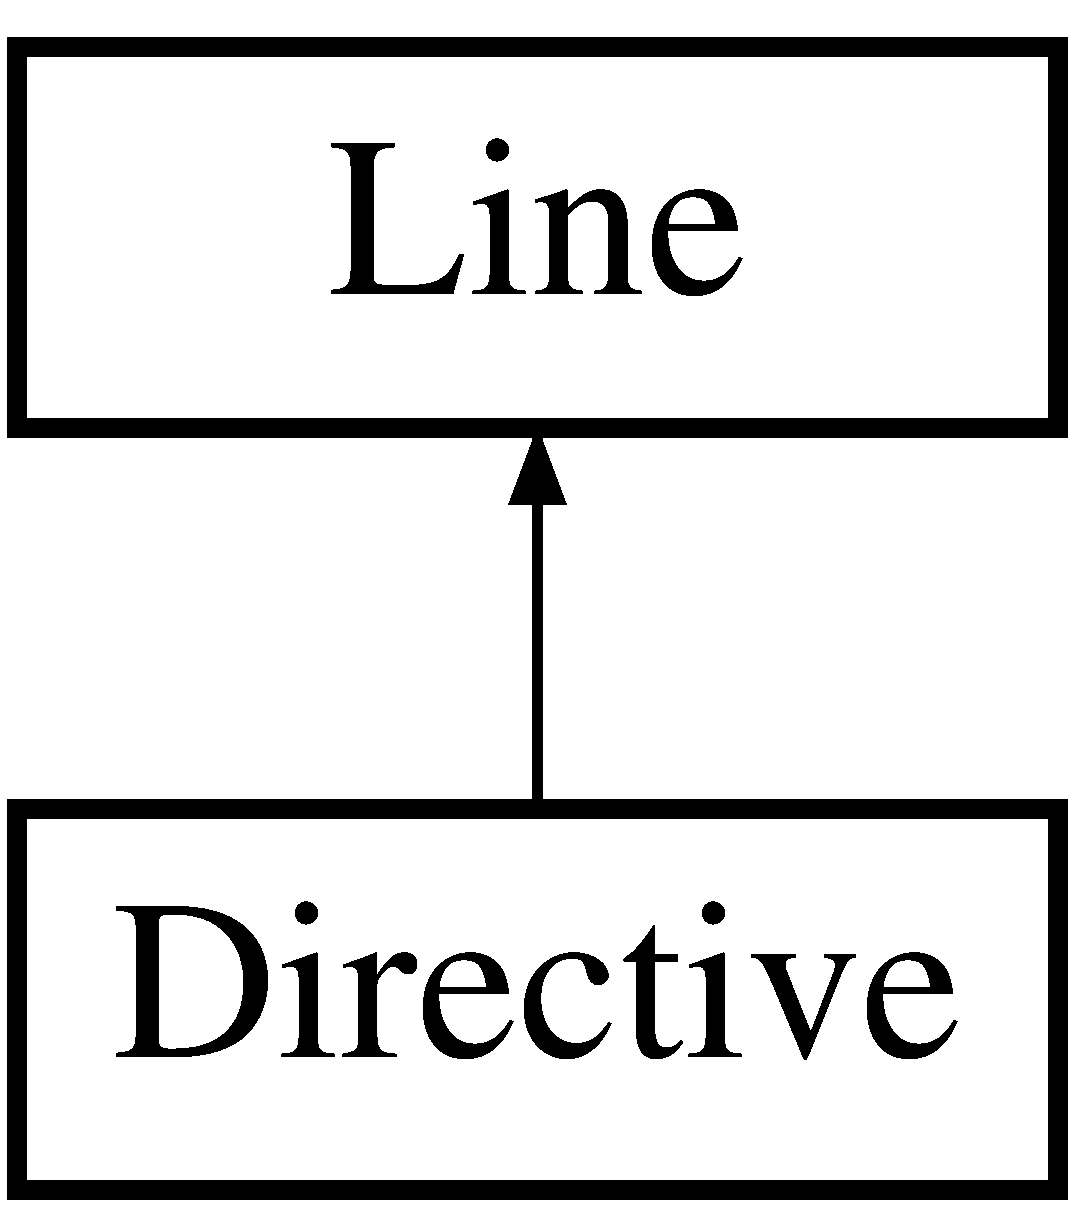
\includegraphics[height=2.000000cm]{classDirective}
\end{center}
\end{figure}
\subsection*{\-Public \-Member \-Functions}
\begin{DoxyCompactItemize}
\item 
\hypertarget{classDirective_a7487120f679e1b4d01843ad6feac7e07}{\hyperlink{classDirective_a7487120f679e1b4d01843ad6feac7e07}{\-Directive} (string)}\label{classDirective_a7487120f679e1b4d01843ad6feac7e07}

\begin{DoxyCompactList}\small\item\em \-Constructor of the \hyperlink{classDirective}{\-Directive}. \end{DoxyCompactList}\item 
\hypertarget{classDirective_ac2f912e3997d9fed8bc289d77fc06305}{\hyperlink{classDirective_ac2f912e3997d9fed8bc289d77fc06305}{\-Directive} (string, string)}\label{classDirective_ac2f912e3997d9fed8bc289d77fc06305}

\begin{DoxyCompactList}\small\item\em \-Constructor of the \hyperlink{classDirective}{\-Directive} with directive, content and an boolean. \end{DoxyCompactList}\item 
\hypertarget{classDirective_adbe3bd8e72354bde2b7d809348d0d527}{\hyperlink{classDirective_adbe3bd8e72354bde2b7d809348d0d527}{\-Directive} (string, string, bool)}\label{classDirective_adbe3bd8e72354bde2b7d809348d0d527}

\begin{DoxyCompactList}\small\item\em \-Constructor of the \hyperlink{classDirective}{\-Directive} with directive, content and an boolean. \end{DoxyCompactList}\item 
\hypertarget{classDirective_aa9a48f09b0472c835ffa366bcff74f51}{virtual \hyperlink{classDirective_aa9a48f09b0472c835ffa366bcff74f51}{$\sim$\-Directive} ()}\label{classDirective_aa9a48f09b0472c835ffa366bcff74f51}

\begin{DoxyCompactList}\small\item\em \-Destructor of the \hyperlink{classDirective}{\-Directive}. \end{DoxyCompactList}\item 
\hypertarget{classDirective_a0d574b0ffc25eb1fbc49032534e7ff44}{virtual t\-\_\-\-Line \hyperlink{classDirective_a0d574b0ffc25eb1fbc49032534e7ff44}{type\-\_\-line} ()}\label{classDirective_a0d574b0ffc25eb1fbc49032534e7ff44}

\begin{DoxyCompactList}\small\item\em get the type of the line \end{DoxyCompactList}\item 
\hypertarget{classDirective_a2fd56d5580ad7a993782649d7867732f}{virtual string \hyperlink{classDirective_a2fd56d5580ad7a993782649d7867732f}{to\-\_\-string} ()}\label{classDirective_a2fd56d5580ad7a993782649d7867732f}

\begin{DoxyCompactList}\small\item\em get the string of the \hyperlink{classDirective}{\-Directive} \end{DoxyCompactList}\item 
\hypertarget{classDirective_aaeb0e95f88f41425718859daeb2116ad}{virtual string \hyperlink{classDirective_aaeb0e95f88f41425718859daeb2116ad}{get\-\_\-content} ()}\label{classDirective_aaeb0e95f88f41425718859daeb2116ad}

\begin{DoxyCompactList}\small\item\em get the string of the \hyperlink{classDirective}{\-Directive} \end{DoxyCompactList}\item 
\hypertarget{classDirective_a59b72d2ebc140e3ac0a0d6d789bb5bba}{virtual void \hyperlink{classDirective_a59b72d2ebc140e3ac0a0d6d789bb5bba}{set\-\_\-content} (string)}\label{classDirective_a59b72d2ebc140e3ac0a0d6d789bb5bba}

\begin{DoxyCompactList}\small\item\em set the string of the \hyperlink{classDirective}{\-Directive} \end{DoxyCompactList}\item 
\hypertarget{classDirective_ae585a212960cc755c057f85533ddc71e}{bool \hyperlink{classDirective_ae585a212960cc755c057f85533ddc71e}{is\-\_\-function} ()}\label{classDirective_ae585a212960cc755c057f85533ddc71e}

\begin{DoxyCompactList}\small\item\em return true if the directive indicate a function \end{DoxyCompactList}\item 
\hypertarget{classDirective_a5c3ac59a9d3bc3c16341124482370843}{virtual t\-\_\-\-Inst \hyperlink{classDirective_a5c3ac59a9d3bc3c16341124482370843}{get\-\_\-type} ()}\label{classDirective_a5c3ac59a9d3bc3c16341124482370843}

\begin{DoxyCompactList}\small\item\em return the type of the instruction \end{DoxyCompactList}\end{DoxyCompactItemize}
\subsection*{\-Public \-Attributes}
\begin{DoxyCompactItemize}
\item 
\hypertarget{classDirective_a3e89203d14d83c6ff8da7a1c49b9a60e}{string {\bfseries \-\_\-dir}}\label{classDirective_a3e89203d14d83c6ff8da7a1c49b9a60e}

\item 
\hypertarget{classDirective_aaeaa71135c6d434d58db763a1e2b70e3}{string {\bfseries \-\_\-value}}\label{classDirective_aaeaa71135c6d434d58db763a1e2b70e3}

\item 
\hypertarget{classDirective_ae9e02b1ecc6a1b5387f5227959984c1f}{bool {\bfseries \-\_\-isfunction}}\label{classDirective_ae9e02b1ecc6a1b5387f5227959984c1f}

\end{DoxyCompactItemize}


\subsection{\-Detailed \-Description}
class representing an \hyperlink{classDirective}{\-Directive} herited by \hyperlink{classLine}{\-Line} 

\-The documentation for this class was generated from the following file\-:\begin{DoxyCompactItemize}
\item 
\hyperlink{Directive_8h}{\-Directive.\-h}\end{DoxyCompactItemize}

\hypertarget{classFunction}{\section{\-Function \-Class \-Reference}
\label{classFunction}\index{\-Function@{\-Function}}
}


class representing a \hyperlink{classFunction}{\-Function} on a program  




{\ttfamily \#include $<$\-Function.\-h$>$}

\subsection*{\-Public \-Member \-Functions}
\begin{DoxyCompactItemize}
\item 
\hypertarget{classFunction_ae206568fd4fd4c885e3ccff76345c4e6}{\hyperlink{classFunction_ae206568fd4fd4c885e3ccff76345c4e6}{\-Function} ()}\label{classFunction_ae206568fd4fd4c885e3ccff76345c4e6}

\begin{DoxyCompactList}\small\item\em \-Constructor of a function. \end{DoxyCompactList}\item 
\hypertarget{classFunction_a3b03f7cf0b75d16edebdda1dee1db6fd}{\hyperlink{classFunction_a3b03f7cf0b75d16edebdda1dee1db6fd}{$\sim$\-Function} ()}\label{classFunction_a3b03f7cf0b75d16edebdda1dee1db6fd}

\begin{DoxyCompactList}\small\item\em \-Destructor of a function. \end{DoxyCompactList}\item 
\hypertarget{classFunction_a39d6ea7220c44d9bb67e2a644ed679d1}{void \hyperlink{classFunction_a39d6ea7220c44d9bb67e2a644ed679d1}{set\-\_\-head} (\hyperlink{classNode}{\-Node} $\ast$)}\label{classFunction_a39d6ea7220c44d9bb67e2a644ed679d1}

\begin{DoxyCompactList}\small\item\em setter of the head of the function \end{DoxyCompactList}\item 
\hypertarget{classFunction_a741002f6a0c79c49afe9cf7c8628159d}{void \hyperlink{classFunction_a741002f6a0c79c49afe9cf7c8628159d}{set\-\_\-end} (\hyperlink{classNode}{\-Node} $\ast$)}\label{classFunction_a741002f6a0c79c49afe9cf7c8628159d}

\begin{DoxyCompactList}\small\item\em setter of the end of the function \end{DoxyCompactList}\item 
\hypertarget{classFunction_ad166c144498bcd0c82efd71a9ce38fd5}{\hyperlink{classNode}{\-Node} $\ast$ \hyperlink{classFunction_ad166c144498bcd0c82efd71a9ce38fd5}{get\-\_\-head} ()}\label{classFunction_ad166c144498bcd0c82efd71a9ce38fd5}

\begin{DoxyCompactList}\small\item\em get the head of the function \end{DoxyCompactList}\item 
\hypertarget{classFunction_a6789e258845ec7b9d2fd922c6291396d}{\hyperlink{classBasic__block}{\-Basic\-\_\-block} $\ast$ {\bfseries get\-\_\-first\-B\-B} ()}\label{classFunction_a6789e258845ec7b9d2fd922c6291396d}

\item 
\hypertarget{classFunction_a57e6d0f497252ac29597e3b65d9f856a}{\hyperlink{classNode}{\-Node} $\ast$ \hyperlink{classFunction_a57e6d0f497252ac29597e3b65d9f856a}{get\-\_\-end} ()}\label{classFunction_a57e6d0f497252ac29597e3b65d9f856a}

\begin{DoxyCompactList}\small\item\em get the end of the function \end{DoxyCompactList}\item 
\hypertarget{classFunction_ade8a6050da83010be473a6581d65a3ce}{void \hyperlink{classFunction_ade8a6050da83010be473a6581d65a3ce}{display} ()}\label{classFunction_ade8a6050da83010be473a6581d65a3ce}

\begin{DoxyCompactList}\small\item\em display the function \end{DoxyCompactList}\item 
\hypertarget{classFunction_a0b62379b4e18c9440963b54d2e8991b0}{int \hyperlink{classFunction_a0b62379b4e18c9440963b54d2e8991b0}{size} ()}\label{classFunction_a0b62379b4e18c9440963b54d2e8991b0}

\begin{DoxyCompactList}\small\item\em get the size of the function \end{DoxyCompactList}\item 
\hypertarget{classFunction_acd08be840c48abd3c0c0c20ca4b5192a}{void \hyperlink{classFunction_acd08be840c48abd3c0c0c20ca4b5192a}{restitution} (string const)}\label{classFunction_acd08be840c48abd3c0c0c20ca4b5192a}

\begin{DoxyCompactList}\small\item\em restitute the function in a file \end{DoxyCompactList}\item 
\hypertarget{classFunction_a833adcab24d31a7787a698b8c6cf61d9}{void {\bfseries add\-\_\-\-B\-B} (\hyperlink{classNode}{\-Node} $\ast$, \hyperlink{classNode}{\-Node} $\ast$, int)}\label{classFunction_a833adcab24d31a7787a698b8c6cf61d9}

\item 
\hypertarget{classFunction_a6094f123294ccbb891fa4145fd5b1b0a}{void \hyperlink{classFunction_a6094f123294ccbb891fa4145fd5b1b0a}{comput\-\_\-basic\-\_\-block} ()}\label{classFunction_a6094f123294ccbb891fa4145fd5b1b0a}

\begin{DoxyCompactList}\small\item\em \-Calculate the basics bolck of the function. \end{DoxyCompactList}\item 
\hypertarget{classFunction_a4ddde4ac1ff488dfcbfcaee71f727a48}{int \hyperlink{classFunction_a4ddde4ac1ff488dfcbfcaee71f727a48}{nbr\-\_\-\-B\-B} ()}\label{classFunction_a4ddde4ac1ff488dfcbfcaee71f727a48}

\begin{DoxyCompactList}\small\item\em get the number of \-Basic block in the function \end{DoxyCompactList}\item 
\hypertarget{classFunction_ae11968b8ca5497526e9448b67823d373}{\hyperlink{classBasic__block}{\-Basic\-\_\-block} $\ast$ \hyperlink{classFunction_ae11968b8ca5497526e9448b67823d373}{get\-\_\-\-B\-B} (int)}\label{classFunction_ae11968b8ca5497526e9448b67823d373}

\begin{DoxyCompactList}\small\item\em get the \-Basic \-Block in the list \end{DoxyCompactList}\item 
\hypertarget{classFunction_a18797dfd75ba34acf0e73b69da8311ec}{list$<$ \hyperlink{classBasic__block}{\-Basic\-\_\-block} $\ast$ $>$\-::iterator {\bfseries bb\-\_\-list\-\_\-begin} ()}\label{classFunction_a18797dfd75ba34acf0e73b69da8311ec}

\item 
\hypertarget{classFunction_a06be1b0a730b4ead3da6bb5529df9788}{list$<$ \hyperlink{classBasic__block}{\-Basic\-\_\-block} $\ast$ $>$\-::iterator {\bfseries bb\-\_\-list\-\_\-end} ()}\label{classFunction_a06be1b0a730b4ead3da6bb5529df9788}

\item 
\hypertarget{classFunction_a1c8830219ce4306c22a933b17f54cc6f}{void \hyperlink{classFunction_a1c8830219ce4306c22a933b17f54cc6f}{comput\-\_\-label} ()}\label{classFunction_a1c8830219ce4306c22a933b17f54cc6f}

\begin{DoxyCompactList}\small\item\em comput labels of the function in list \end{DoxyCompactList}\item 
\hypertarget{classFunction_a4b2e9837c4b506b3c7a6d1488d9914d1}{\hyperlink{classLabel}{\-Label} $\ast$ \hyperlink{classFunction_a4b2e9837c4b506b3c7a6d1488d9914d1}{get\-\_\-label} (int)}\label{classFunction_a4b2e9837c4b506b3c7a6d1488d9914d1}

\begin{DoxyCompactList}\small\item\em get all labels of the function \end{DoxyCompactList}\item 
\hypertarget{classFunction_a3f3807e12e695ffe23e1ef44edcd262b}{int \hyperlink{classFunction_a3f3807e12e695ffe23e1ef44edcd262b}{nbr\-\_\-label} ()}\label{classFunction_a3f3807e12e695ffe23e1ef44edcd262b}

\begin{DoxyCompactList}\small\item\em get the size of the list label \end{DoxyCompactList}\item 
\hypertarget{classFunction_ae55c0232d0eced8830daf57293229db8}{\hyperlink{classBasic__block}{\-Basic\-\_\-block} $\ast$ \hyperlink{classFunction_ae55c0232d0eced8830daf57293229db8}{find\-\_\-label\-\_\-\-B\-B} (\hyperlink{classOPLabel}{\-O\-P\-Label} $\ast$)}\label{classFunction_ae55c0232d0eced8830daf57293229db8}

\begin{DoxyCompactList}\small\item\em \-Get the basic block corresponding to the label. \end{DoxyCompactList}\item 
\hypertarget{classFunction_a3c52c8cb82e0137f02771331018b655c}{void \hyperlink{classFunction_a3c52c8cb82e0137f02771331018b655c}{comput\-\_\-succ\-\_\-pred\-\_\-\-B\-B} ()}\label{classFunction_a3c52c8cb82e0137f02771331018b655c}

\begin{DoxyCompactList}\small\item\em \-Associate for each \-Basic block its successors. \end{DoxyCompactList}\item 
\hypertarget{classFunction_aaa0d06640a5075c416106a88bd9a833a}{void \hyperlink{classFunction_aaa0d06640a5075c416106a88bd9a833a}{test} ()}\label{classFunction_aaa0d06640a5075c416106a88bd9a833a}

\begin{DoxyCompactList}\small\item\em method to test other methods \end{DoxyCompactList}\end{DoxyCompactItemize}


\subsection{\-Detailed \-Description}
class representing a \hyperlink{classFunction}{\-Function} on a program 

\-The documentation for this class was generated from the following file\-:\begin{DoxyCompactItemize}
\item 
\hyperlink{Function_8h}{\-Function.\-h}\end{DoxyCompactItemize}

\hypertarget{classInstruction}{\section{\-Instruction \-Class \-Reference}
\label{classInstruction}\index{\-Instruction@{\-Instruction}}
}


class representing an instruction which herited by \hyperlink{classLine}{\-Line}  




{\ttfamily \#include $<$\-Instruction.\-h$>$}

\-Inheritance diagram for \-Instruction\-:\begin{figure}[H]
\begin{center}
\leavevmode
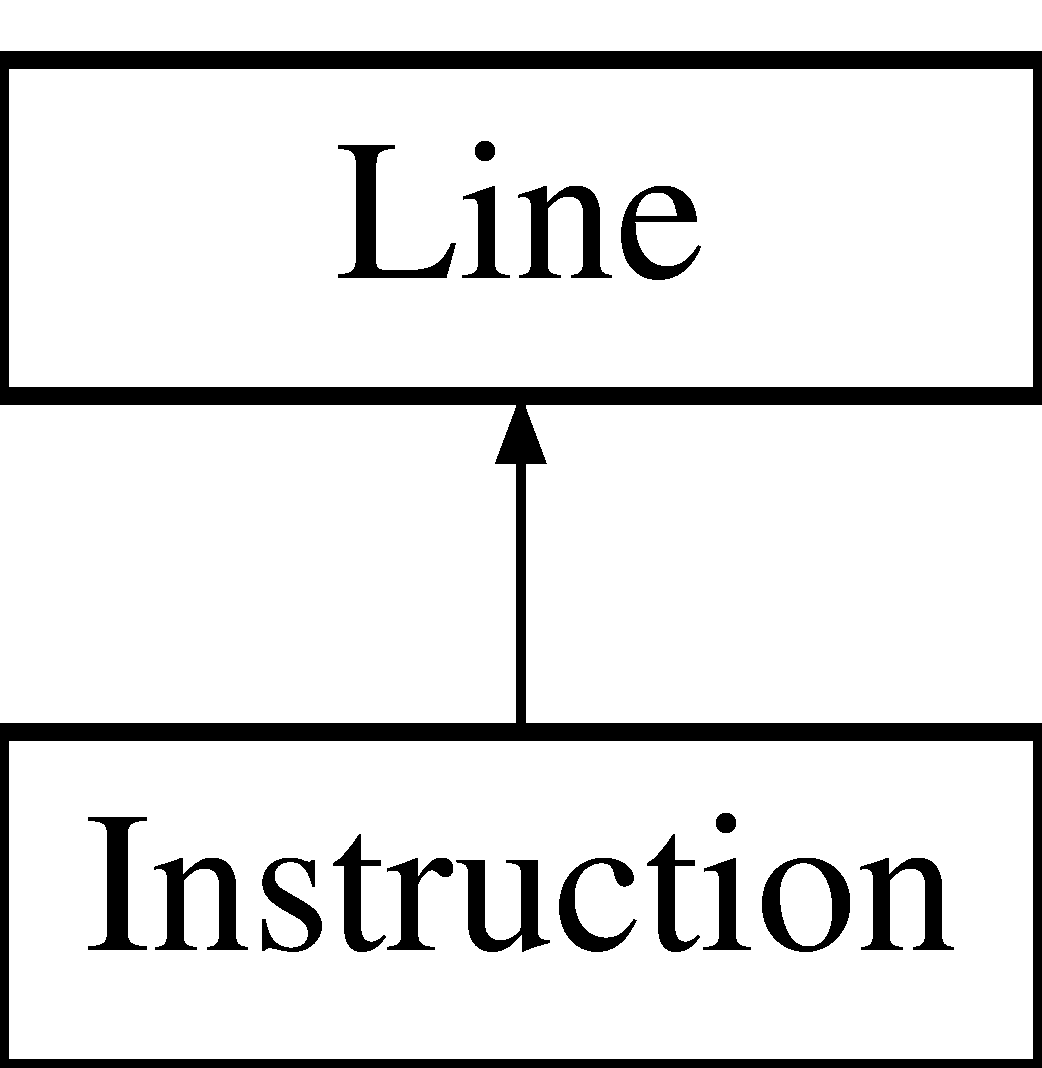
\includegraphics[height=2.000000cm]{classInstruction}
\end{center}
\end{figure}
\subsection*{\-Public \-Member \-Functions}
\begin{DoxyCompactItemize}
\item 
\hypertarget{classInstruction_a055c483afc0512b68f6211fdbb6774ba}{\hyperlink{classInstruction_a055c483afc0512b68f6211fdbb6774ba}{\-Instruction} (string, t\-\_\-\-Operator, t\-\_\-\-Inst, \hyperlink{classOperand}{\-Operand} $\ast$, \hyperlink{classOperand}{\-Operand} $\ast$, \hyperlink{classOperand}{\-Operand} $\ast$)}\label{classInstruction_a055c483afc0512b68f6211fdbb6774ba}

\begin{DoxyCompactList}\small\item\em \-Constructor of the class instruction. \end{DoxyCompactList}\item 
\hypertarget{classInstruction_a2f1ed1606d4090b8a4c255e3af9e34c8}{\hyperlink{classInstruction_a2f1ed1606d4090b8a4c255e3af9e34c8}{\-Instruction} (t\-\_\-\-Operator, \hyperlink{classOperand}{\-Operand} $\ast$, \hyperlink{classOperand}{\-Operand} $\ast$, \hyperlink{classOperand}{\-Operand} $\ast$)}\label{classInstruction_a2f1ed1606d4090b8a4c255e3af9e34c8}

\begin{DoxyCompactList}\small\item\em \-Constructor with 3 \-Operands of the class instruction. \end{DoxyCompactList}\item 
\hypertarget{classInstruction_a0b1ed4432c9c5823ee9e522c7d11bb5f}{\hyperlink{classInstruction_a0b1ed4432c9c5823ee9e522c7d11bb5f}{\-Instruction} (t\-\_\-\-Operator, \hyperlink{classOperand}{\-Operand} $\ast$, \hyperlink{classOperand}{\-Operand} $\ast$)}\label{classInstruction_a0b1ed4432c9c5823ee9e522c7d11bb5f}

\begin{DoxyCompactList}\small\item\em \-Constructor with 2 \-Operands of the class instruction. \end{DoxyCompactList}\item 
\hypertarget{classInstruction_a6ae2a4dd83500f9d538a653823161b1c}{\hyperlink{classInstruction_a6ae2a4dd83500f9d538a653823161b1c}{\-Instruction} (t\-\_\-\-Operator, \hyperlink{classOperand}{\-Operand} $\ast$)}\label{classInstruction_a6ae2a4dd83500f9d538a653823161b1c}

\begin{DoxyCompactList}\small\item\em \-Constructor with 1 \hyperlink{classOperand}{\-Operand} of the class instruction. \end{DoxyCompactList}\item 
\hypertarget{classInstruction_ab2d989cc18e9bf0eeee194a7614514fa}{\hyperlink{classInstruction_ab2d989cc18e9bf0eeee194a7614514fa}{\-Instruction} (t\-\_\-\-Operator)}\label{classInstruction_ab2d989cc18e9bf0eeee194a7614514fa}

\begin{DoxyCompactList}\small\item\em \-Constructor without \-Operands of the class instruction. \end{DoxyCompactList}\item 
\hypertarget{classInstruction_a3f1031e811b710787678f8faf8cc9672}{virtual \hyperlink{classInstruction_a3f1031e811b710787678f8faf8cc9672}{$\sim$\-Instruction} ()}\label{classInstruction_a3f1031e811b710787678f8faf8cc9672}

\begin{DoxyCompactList}\small\item\em \-Destructor of the class instruction. \end{DoxyCompactList}\item 
\hypertarget{classInstruction_a8b475d42fd5e8c258823bc2d5b5da3b5}{\hyperlink{classOperand}{\-Operand} $\ast$ \hyperlink{classInstruction_a8b475d42fd5e8c258823bc2d5b5da3b5}{get\-\_\-op1} ()}\label{classInstruction_a8b475d42fd5e8c258823bc2d5b5da3b5}

\begin{DoxyCompactList}\small\item\em \-Get the first operand value accessor of the operand. \end{DoxyCompactList}\item 
\hypertarget{classInstruction_a4dd27924105fba4ba68d4b22747ad835}{void \hyperlink{classInstruction_a4dd27924105fba4ba68d4b22747ad835}{set\-\_\-op1} (\hyperlink{classOperand}{\-Operand} $\ast$o)}\label{classInstruction_a4dd27924105fba4ba68d4b22747ad835}

\begin{DoxyCompactList}\small\item\em set the first operand value setter of the operand \end{DoxyCompactList}\item 
\hypertarget{classInstruction_ac67b313ca1836f911735fffb66eb7379}{\hyperlink{classOperand}{\-Operand} $\ast$ \hyperlink{classInstruction_ac67b313ca1836f911735fffb66eb7379}{get\-\_\-op2} ()}\label{classInstruction_ac67b313ca1836f911735fffb66eb7379}

\begin{DoxyCompactList}\small\item\em \-Get the second operand value accessor of the operand. \end{DoxyCompactList}\item 
\hypertarget{classInstruction_a4bee8cf0b4687a56c244a8bb864ed13b}{void \hyperlink{classInstruction_a4bee8cf0b4687a56c244a8bb864ed13b}{set\-\_\-op2} (\hyperlink{classOperand}{\-Operand} $\ast$o)}\label{classInstruction_a4bee8cf0b4687a56c244a8bb864ed13b}

\begin{DoxyCompactList}\small\item\em set the second operand value setter of the operand \end{DoxyCompactList}\item 
\hypertarget{classInstruction_adf81522ab8abde73f5fc575cebeedcbd}{\hyperlink{classOperand}{\-Operand} $\ast$ \hyperlink{classInstruction_adf81522ab8abde73f5fc575cebeedcbd}{get\-\_\-op3} ()}\label{classInstruction_adf81522ab8abde73f5fc575cebeedcbd}

\begin{DoxyCompactList}\small\item\em \-Get the third operand value accessor of the operand. \end{DoxyCompactList}\item 
\hypertarget{classInstruction_a010bb7c48922d36b06b563bb1f45bfa3}{void \hyperlink{classInstruction_a010bb7c48922d36b06b563bb1f45bfa3}{set\-\_\-op3} (\hyperlink{classOperand}{\-Operand} $\ast$o)}\label{classInstruction_a010bb7c48922d36b06b563bb1f45bfa3}

\begin{DoxyCompactList}\small\item\em set the third operand value setter of the operand \end{DoxyCompactList}\item 
\hypertarget{classInstruction_a1195d03eb4ff6024b20cd2cec1c8a1e0}{t\-\_\-\-Operator \hyperlink{classInstruction_a1195d03eb4ff6024b20cd2cec1c8a1e0}{get\-\_\-opcode} ()}\label{classInstruction_a1195d03eb4ff6024b20cd2cec1c8a1e0}

\begin{DoxyCompactList}\small\item\em get the \-Opcode value accessor of the opcode \end{DoxyCompactList}\item 
\hypertarget{classInstruction_aeba180e03a3ac7f7ecba7635d454566f}{string \hyperlink{classInstruction_aeba180e03a3ac7f7ecba7635d454566f}{string\-\_\-opcode} ()}\label{classInstruction_aeba180e03a3ac7f7ecba7635d454566f}

\begin{DoxyCompactList}\small\item\em get the string \-Opcode value accessor of the string opcode \end{DoxyCompactList}\item 
\hypertarget{classInstruction_a49524f35c4ade25c663d798e3a5df2cb}{void \hyperlink{classInstruction_a49524f35c4ade25c663d798e3a5df2cb}{set\-\_\-opcode} (t\-\_\-\-Operator newop)}\label{classInstruction_a49524f35c4ade25c663d798e3a5df2cb}

\begin{DoxyCompactList}\small\item\em set the opcode value setter of the opcode \end{DoxyCompactList}\item 
\hypertarget{classInstruction_a86e8d9627ad78884d75481693a6196ef}{t\-\_\-\-Format \hyperlink{classInstruction_a86e8d9627ad78884d75481693a6196ef}{get\-\_\-format} ()}\label{classInstruction_a86e8d9627ad78884d75481693a6196ef}

\begin{DoxyCompactList}\small\item\em get the format of the \hyperlink{classInstruction}{\-Instruction} accessor of the format \end{DoxyCompactList}\item 
\hypertarget{classInstruction_ae619398c5531b1f2042fb4caa893cdee}{virtual t\-\_\-\-Inst \hyperlink{classInstruction_ae619398c5531b1f2042fb4caa893cdee}{get\-\_\-type} ()}\label{classInstruction_ae619398c5531b1f2042fb4caa893cdee}

\begin{DoxyCompactList}\small\item\em get the \-Type of the \hyperlink{classInstruction}{\-Instruction} accessor of the \-Type \end{DoxyCompactList}\item 
\hypertarget{classInstruction_adcab5ded0016e613826be14514abbcc8}{virtual t\-\_\-\-Line \hyperlink{classInstruction_adcab5ded0016e613826be14514abbcc8}{type\-\_\-line} ()}\label{classInstruction_adcab5ded0016e613826be14514abbcc8}

\begin{DoxyCompactList}\small\item\em get the type of the line \end{DoxyCompactList}\item 
\hypertarget{classInstruction_aed87de5e9259f4f15dc885425528f1fe}{virtual string \hyperlink{classInstruction_aed87de5e9259f4f15dc885425528f1fe}{to\-\_\-string} ()}\label{classInstruction_aed87de5e9259f4f15dc885425528f1fe}

\begin{DoxyCompactList}\small\item\em get the name string instruction \end{DoxyCompactList}\item 
\hypertarget{classInstruction_a5b258bf1dfb9f6fa2fff0af0e7c211d8}{virtual string \hyperlink{classInstruction_a5b258bf1dfb9f6fa2fff0af0e7c211d8}{get\-\_\-content} ()}\label{classInstruction_a5b258bf1dfb9f6fa2fff0af0e7c211d8}

\begin{DoxyCompactList}\small\item\em get the string of the instruction \end{DoxyCompactList}\item 
\hypertarget{classInstruction_aec1a1ab575287b532fb8d43cfa364e30}{virtual void \hyperlink{classInstruction_aec1a1ab575287b532fb8d43cfa364e30}{set\-\_\-content} (string)}\label{classInstruction_aec1a1ab575287b532fb8d43cfa364e30}

\begin{DoxyCompactList}\small\item\em set the string of the instruction \end{DoxyCompactList}\item 
\hypertarget{classInstruction_a2d2d966c6269e1e0dbfbeb8aabafeeb4}{string \hyperlink{classInstruction_a2d2d966c6269e1e0dbfbeb8aabafeeb4}{string\-\_\-form} ()}\label{classInstruction_a2d2d966c6269e1e0dbfbeb8aabafeeb4}

\begin{DoxyCompactList}\small\item\em set the string format \end{DoxyCompactList}\item 
\hypertarget{classInstruction_ac2d81dcf8ddd82e31262c7adb1a0df69}{string \hyperlink{classInstruction_ac2d81dcf8ddd82e31262c7adb1a0df69}{string\-\_\-type} ()}\label{classInstruction_ac2d81dcf8ddd82e31262c7adb1a0df69}

\begin{DoxyCompactList}\small\item\em set the string \-Type of instruction \end{DoxyCompactList}\item 
\hypertarget{classInstruction_aa081b0cc47a8f62c5cef19db820ffae5}{bool {\bfseries reads\-\_\-in} (int dst)}\label{classInstruction_aa081b0cc47a8f62c5cef19db820ffae5}

\item 
\hypertarget{classInstruction_a4000963498afab8b78820a58a77e0a25}{bool {\bfseries writes\-\_\-in} (int dst)}\label{classInstruction_a4000963498afab8b78820a58a77e0a25}

\item 
t\-\_\-\-Dep \hyperlink{classInstruction_ac8d86b800140a08cb03d82f83f363fa4}{is\-\_\-dependant} (\hyperlink{classInstruction}{\-Instruction} $\ast$i2)
\begin{DoxyCompactList}\small\item\em get the dependance between the current instruction and i2 \end{DoxyCompactList}\item 
bool \hyperlink{classInstruction_ae5d54f535adab416c53eb0ff6a438804}{is\-\_\-dep\-\_\-\-R\-A\-W1} (\hyperlink{classInstruction}{\-Instruction} $\ast$i2)
\begin{DoxyCompactList}\small\item\em get the information if there is dependance \-R\-A\-W between the current instruction and i2 \end{DoxyCompactList}\item 
bool \hyperlink{classInstruction_aa28ae5f427ee02c96466f1ac68060f87}{is\-\_\-dep\-\_\-\-R\-A\-W2} (\hyperlink{classInstruction}{\-Instruction} $\ast$i2)
\begin{DoxyCompactList}\small\item\em get the information if there is dependance \-R\-A\-W between the current instruction and the first source operand of i2 \end{DoxyCompactList}\item 
bool \hyperlink{classInstruction_a4c902c5a8fdc8c8841ec24f389605fd5}{is\-\_\-dep\-\_\-\-R\-A\-W} (\hyperlink{classInstruction}{\-Instruction} $\ast$i2)
\begin{DoxyCompactList}\small\item\em get the information if there is dependance \-R\-A\-W between the current instruction and i2 \end{DoxyCompactList}\item 
bool \hyperlink{classInstruction_a36c0faedd74af14b403ba7063af5d07f}{is\-\_\-dep\-\_\-\-W\-A\-R1} (\hyperlink{classInstruction}{\-Instruction} $\ast$i2)
\begin{DoxyCompactList}\small\item\em test if there is dependance \-W\-A\-R between the first source operande of the current instruction if any and the destination register operande i2 if any \end{DoxyCompactList}\item 
bool \hyperlink{classInstruction_a04471df677984f67ec13de88f55e3703}{is\-\_\-dep\-\_\-\-W\-A\-R2} (\hyperlink{classInstruction}{\-Instruction} $\ast$i2)
\begin{DoxyCompactList}\small\item\em test if there is dependance \-W\-A\-R between the second source operande of the current instruction if any and the destination register operande i2 if any \end{DoxyCompactList}\item 
bool \hyperlink{classInstruction_ae79b239c6ab30a15064b5a00944ad65a}{is\-\_\-dep\-\_\-\-W\-A\-R} (\hyperlink{classInstruction}{\-Instruction} $\ast$i2)
\begin{DoxyCompactList}\small\item\em get the information if there is dependance \-W\-A\-R between the current instruction and i2 \end{DoxyCompactList}\item 
bool \hyperlink{classInstruction_a30c159faa5c462bb2c7ae7562c9c8254}{is\-\_\-dep\-\_\-\-W\-A\-W} (\hyperlink{classInstruction}{\-Instruction} $\ast$i2)
\begin{DoxyCompactList}\small\item\em get the information if there is dependance \-W\-A\-W between the current instruction and i2 \end{DoxyCompactList}\item 
bool \hyperlink{classInstruction_a28526bda91b964d7fd81f85cee02c624}{is\-\_\-dep\-\_\-\-M\-E\-M} (\hyperlink{classInstruction}{\-Instruction} $\ast$i2)
\begin{DoxyCompactList}\small\item\em test if there is dependance \-M\-E\-M\-D\-E\-P between the current instruction and i2 \end{DoxyCompactList}\item 
int \hyperlink{classInstruction_a044a281355f25375a7765f24bdf614f3}{get\-\_\-nb\-Op} ()
\begin{DoxyCompactList}\small\item\em get the number of operand \end{DoxyCompactList}\item 
\hypertarget{classInstruction_a6ff2d531dffa43d3db22194459336d33}{void \hyperlink{classInstruction_a6ff2d531dffa43d3db22194459336d33}{set\-\_\-number\-\_\-oper} (int)}\label{classInstruction_a6ff2d531dffa43d3db22194459336d33}

\begin{DoxyCompactList}\small\item\em set the number of operand \end{DoxyCompactList}\item 
\hypertarget{classInstruction_adb43e7019987daebb3970335aba695cc}{\hyperlink{classOPRegister}{\-O\-P\-Register} $\ast$ \hyperlink{classInstruction_adb43e7019987daebb3970335aba695cc}{get\-\_\-reg\-\_\-dst} ()}\label{classInstruction_adb43e7019987daebb3970335aba695cc}

\begin{DoxyCompactList}\small\item\em get the regiter destination of the instruction \end{DoxyCompactList}\item 
\hypertarget{classInstruction_ac353a6ad2b3f3b1aee179d5910b5127b}{\hyperlink{classOPRegister}{\-O\-P\-Register} $\ast$ \hyperlink{classInstruction_ac353a6ad2b3f3b1aee179d5910b5127b}{get\-\_\-reg\-\_\-src1} ()}\label{classInstruction_ac353a6ad2b3f3b1aee179d5910b5127b}

\begin{DoxyCompactList}\small\item\em get the first register source of the instruction \end{DoxyCompactList}\item 
\hypertarget{classInstruction_a0eb007b1b0a038610e71a58af3bb6438}{\hyperlink{classOPRegister}{\-O\-P\-Register} $\ast$ \hyperlink{classInstruction_a0eb007b1b0a038610e71a58af3bb6438}{get\-\_\-reg\-\_\-src2} ()}\label{classInstruction_a0eb007b1b0a038610e71a58af3bb6438}

\begin{DoxyCompactList}\small\item\em get the second register source of the instruction \end{DoxyCompactList}\item 
\hypertarget{classInstruction_a2fb436e52a0cc89e7ec08bf0e105bba3}{void \hyperlink{classInstruction_a2fb436e52a0cc89e7ec08bf0e105bba3}{set\-\_\-next} (\hyperlink{classInstruction}{\-Instruction} $\ast$)}\label{classInstruction_a2fb436e52a0cc89e7ec08bf0e105bba3}

\begin{DoxyCompactList}\small\item\em get the successor of the \hyperlink{classInstruction}{\-Instruction} \end{DoxyCompactList}\item 
\hypertarget{classInstruction_ab8f6e21bc94df2198678a3cdbcfaa12e}{void \hyperlink{classInstruction_ab8f6e21bc94df2198678a3cdbcfaa12e}{set\-\_\-link\-\_\-succ\-\_\-pred} (\hyperlink{classInstruction}{\-Instruction} $\ast$)}\label{classInstruction_ab8f6e21bc94df2198678a3cdbcfaa12e}

\begin{DoxyCompactList}\small\item\em set the parameter as successor and this as predecessor of the parameter \end{DoxyCompactList}\item 
\hypertarget{classInstruction_a93d5d6186afcf358c5a21f4c57a0d72e}{\hyperlink{classInstruction}{\-Instruction} $\ast$ \hyperlink{classInstruction_a93d5d6186afcf358c5a21f4c57a0d72e}{get\-\_\-next} ()}\label{classInstruction_a93d5d6186afcf358c5a21f4c57a0d72e}

\begin{DoxyCompactList}\small\item\em get the successor of the \hyperlink{classInstruction}{\-Instruction} \end{DoxyCompactList}\item 
\hypertarget{classInstruction_a69d2992a0eb1fbe5fb6a38b52e13a804}{void \hyperlink{classInstruction_a69d2992a0eb1fbe5fb6a38b52e13a804}{set\-\_\-prev} (\hyperlink{classInstruction}{\-Instruction} $\ast$)}\label{classInstruction_a69d2992a0eb1fbe5fb6a38b52e13a804}

\begin{DoxyCompactList}\small\item\em setter of the predecessor of the \hyperlink{classInstruction}{\-Instruction} \end{DoxyCompactList}\item 
\hypertarget{classInstruction_afd6f27235469926b1e7979220495a6f0}{\hyperlink{classInstruction}{\-Instruction} $\ast$ \hyperlink{classInstruction_afd6f27235469926b1e7979220495a6f0}{get\-\_\-prev} ()}\label{classInstruction_afd6f27235469926b1e7979220495a6f0}

\begin{DoxyCompactList}\small\item\em get the predecessor of the \hyperlink{classInstruction}{\-Instruction} \end{DoxyCompactList}\item 
\hypertarget{classInstruction_a3121dad231e2b4c27ac3cae6c8627ece}{void \hyperlink{classInstruction_a3121dad231e2b4c27ac3cae6c8627ece}{add\-\_\-pred\-\_\-dep} (\hyperlink{structdep}{dep} $\ast$)}\label{classInstruction_a3121dad231e2b4c27ac3cae6c8627ece}

\begin{DoxyCompactList}\small\item\em add a type of a dep with a predecessor instruction to the dependance type list \end{DoxyCompactList}\item 
\hypertarget{classInstruction_ab32531f8dd490b1c8396b6723f87bfae}{\hyperlink{structdep}{dep} $\ast$ \hyperlink{classInstruction_ab32531f8dd490b1c8396b6723f87bfae}{get\-\_\-pred\-\_\-dep} (int i)}\label{classInstruction_ab32531f8dd490b1c8396b6723f87bfae}

\begin{DoxyCompactList}\small\item\em get the dependance type with the ith predecessor instruction of the current instruction \end{DoxyCompactList}\item 
\hypertarget{classInstruction_acefc258dbcf45c19136dc86e47a82c0e}{void \hyperlink{classInstruction_acefc258dbcf45c19136dc86e47a82c0e}{add\-\_\-succ\-\_\-dep} (\hyperlink{structdep}{dep} $\ast$)}\label{classInstruction_acefc258dbcf45c19136dc86e47a82c0e}

\begin{DoxyCompactList}\small\item\em add a type of a dep with a successor instruction to list of the dependance type of successors \end{DoxyCompactList}\item 
\hypertarget{classInstruction_a2c6f13ddda889e4e2b8b69897de6b733}{list$<$ \hyperlink{structdep}{dep} $\ast$ $>$\-::iterator {\bfseries succ\-\_\-begin} ()}\label{classInstruction_a2c6f13ddda889e4e2b8b69897de6b733}

\item 
\hypertarget{classInstruction_a0800ca0afbbc783b57170d981d406fb6}{list$<$ \hyperlink{structdep}{dep} $\ast$ $>$\-::iterator {\bfseries succ\-\_\-end} ()}\label{classInstruction_a0800ca0afbbc783b57170d981d406fb6}

\item 
\hypertarget{classInstruction_ad3bb47ea5f9e4b975e0191d6c96ffc30}{\hyperlink{structdep}{dep} $\ast$ \hyperlink{classInstruction_ad3bb47ea5f9e4b975e0191d6c96ffc30}{get\-\_\-succ\-\_\-dep} (int i)}\label{classInstruction_ad3bb47ea5f9e4b975e0191d6c96ffc30}

\begin{DoxyCompactList}\small\item\em get the dependance type with ith successor instruction of the current instruction \end{DoxyCompactList}\item 
\hypertarget{classInstruction_ab2d8c29efa78ec3c1a70f154a8c2f068}{int \hyperlink{classInstruction_ab2d8c29efa78ec3c1a70f154a8c2f068}{get\-\_\-nb\-\_\-succ} ()}\label{classInstruction_ab2d8c29efa78ec3c1a70f154a8c2f068}

\begin{DoxyCompactList}\small\item\em get the number of successor of the \hyperlink{classInstruction}{\-Instruction} \end{DoxyCompactList}\item 
\hypertarget{classInstruction_a9e56e8e2c857abc409f27af9f80f9595}{int \hyperlink{classInstruction_a9e56e8e2c857abc409f27af9f80f9595}{get\-\_\-nb\-\_\-pred} ()}\label{classInstruction_a9e56e8e2c857abc409f27af9f80f9595}

\begin{DoxyCompactList}\small\item\em get the number of predecessor of the \hyperlink{classInstruction}{\-Instruction} \end{DoxyCompactList}\item 
\hypertarget{classInstruction_a14c5f91c242a5b58eda9f123ad331cbe}{int \hyperlink{classInstruction_a14c5f91c242a5b58eda9f123ad331cbe}{get\-\_\-index} ()}\label{classInstruction_a14c5f91c242a5b58eda9f123ad331cbe}

\begin{DoxyCompactList}\small\item\em get the index of instruction \end{DoxyCompactList}\item 
\hypertarget{classInstruction_af1608cfea660c46e8a8b4bbac948406a}{void \hyperlink{classInstruction_af1608cfea660c46e8a8b4bbac948406a}{set\-\_\-index} (int)}\label{classInstruction_af1608cfea660c46e8a8b4bbac948406a}

\begin{DoxyCompactList}\small\item\em set the index of instruction \end{DoxyCompactList}\item 
\hypertarget{classInstruction_aab8e6a16b8bab5ca90b554086cc3c825}{bool \hyperlink{classInstruction_aab8e6a16b8bab5ca90b554086cc3c825}{is\-\_\-branch} ()}\label{classInstruction_aab8e6a16b8bab5ca90b554086cc3c825}

\begin{DoxyCompactList}\small\item\em test if the instruction is a branch \end{DoxyCompactList}\item 
\hypertarget{classInstruction_ab2a6352a09271a588f6930852a361f67}{bool \hyperlink{classInstruction_ab2a6352a09271a588f6930852a361f67}{is\-\_\-call} ()}\label{classInstruction_ab2a6352a09271a588f6930852a361f67}

\begin{DoxyCompactList}\small\item\em test if the instruction is a call \end{DoxyCompactList}\item 
\hypertarget{classInstruction_a1b607074554bc160142786c125bde530}{bool \hyperlink{classInstruction_a1b607074554bc160142786c125bde530}{is\-\_\-cond\-\_\-branch} ()}\label{classInstruction_a1b607074554bc160142786c125bde530}

\begin{DoxyCompactList}\small\item\em test if the instruction is a conditionnal branch \end{DoxyCompactList}\item 
\hypertarget{classInstruction_affdf2382cd36277fb4427cd3b07c1402}{bool \hyperlink{classInstruction_affdf2382cd36277fb4427cd3b07c1402}{is\-\_\-indirect\-\_\-branch} ()}\label{classInstruction_affdf2382cd36277fb4427cd3b07c1402}

\begin{DoxyCompactList}\small\item\em test if the instruction a branch and the target adress is in a register \end{DoxyCompactList}\item 
\hypertarget{classInstruction_a1c79865faf9baa4d70edf81e956d952d}{bool {\bfseries is\-\_\-mem} ()}\label{classInstruction_a1c79865faf9baa4d70edf81e956d952d}

\item 
\hypertarget{classInstruction_aee32f4bb91480afc74375beb139af4d6}{bool \hyperlink{classInstruction_aee32f4bb91480afc74375beb139af4d6}{is\-\_\-mem\-\_\-load} ()}\label{classInstruction_aee32f4bb91480afc74375beb139af4d6}

\begin{DoxyCompactList}\small\item\em test if the instruction is a memory access that reads a value \end{DoxyCompactList}\item 
\hypertarget{classInstruction_a4455144397d239eb61bcfa2b0e16bf67}{bool \hyperlink{classInstruction_a4455144397d239eb61bcfa2b0e16bf67}{is\-\_\-mem\-\_\-store} ()}\label{classInstruction_a4455144397d239eb61bcfa2b0e16bf67}

\begin{DoxyCompactList}\small\item\em test if the instruction is a memory access that writes a value \end{DoxyCompactList}\item 
\hypertarget{classInstruction_ac2988d2fb858b720e009da03120ae4c7}{int \hyperlink{classInstruction_ac2988d2fb858b720e009da03120ae4c7}{get\-\_\-latency} ()}\label{classInstruction_ac2988d2fb858b720e009da03120ae4c7}

\begin{DoxyCompactList}\small\item\em test if the instruction is a memory access that writes a value \end{DoxyCompactList}\item 
\hypertarget{classInstruction_af489e680ae3c69fd12b0a23e959172e5}{void {\bfseries print\-\_\-succ\-\_\-dep} ()}\label{classInstruction_af489e680ae3c69fd12b0a23e959172e5}

\end{DoxyCompactItemize}
\subsection*{\-Static \-Public \-Member \-Functions}
\begin{DoxyCompactItemize}
\item 
\hypertarget{classInstruction_ae309ff37d134500f75e1180182b02a6b}{static bool {\bfseries is\-\_\-writed\-\_\-between} (int dst, \hyperlink{classInstruction}{\-Instruction} $\ast$i1, \hyperlink{classInstruction}{\-Instruction} $\ast$i2exclu)}\label{classInstruction_ae309ff37d134500f75e1180182b02a6b}

\end{DoxyCompactItemize}


\subsection{\-Detailed \-Description}
class representing an instruction which herited by \hyperlink{classLine}{\-Line} 

\subsection{\-Member \-Function \-Documentation}
\hypertarget{classInstruction_a044a281355f25375a7765f24bdf614f3}{\index{\-Instruction@{\-Instruction}!get\-\_\-nb\-Op@{get\-\_\-nb\-Op}}
\index{get\-\_\-nb\-Op@{get\-\_\-nb\-Op}!Instruction@{\-Instruction}}
\subsubsection[{get\-\_\-nb\-Op}]{\setlength{\rightskip}{0pt plus 5cm}int {\bf \-Instruction\-::get\-\_\-nb\-Op} (
\begin{DoxyParamCaption}
{}
\end{DoxyParamCaption}
)}}\label{classInstruction_a044a281355f25375a7765f24bdf614f3}


get the number of operand 

\begin{DoxyReturn}{\-Returns}
return the number of operand 
\end{DoxyReturn}
\hypertarget{classInstruction_a28526bda91b964d7fd81f85cee02c624}{\index{\-Instruction@{\-Instruction}!is\-\_\-dep\-\_\-\-M\-E\-M@{is\-\_\-dep\-\_\-\-M\-E\-M}}
\index{is\-\_\-dep\-\_\-\-M\-E\-M@{is\-\_\-dep\-\_\-\-M\-E\-M}!Instruction@{\-Instruction}}
\subsubsection[{is\-\_\-dep\-\_\-\-M\-E\-M}]{\setlength{\rightskip}{0pt plus 5cm}bool {\bf \-Instruction\-::is\-\_\-dep\-\_\-\-M\-E\-M} (
\begin{DoxyParamCaption}
\item[{{\bf \-Instruction} $\ast$}]{i2}
\end{DoxyParamCaption}
)}}\label{classInstruction_a28526bda91b964d7fd81f85cee02c624}


test if there is dependance \-M\-E\-M\-D\-E\-P between the current instruction and i2 

\begin{DoxyReturn}{\-Returns}
return true if there is a \-M\-E\-M\-D\-E\-P dependance 
\end{DoxyReturn}
\hypertarget{classInstruction_a4c902c5a8fdc8c8841ec24f389605fd5}{\index{\-Instruction@{\-Instruction}!is\-\_\-dep\-\_\-\-R\-A\-W@{is\-\_\-dep\-\_\-\-R\-A\-W}}
\index{is\-\_\-dep\-\_\-\-R\-A\-W@{is\-\_\-dep\-\_\-\-R\-A\-W}!Instruction@{\-Instruction}}
\subsubsection[{is\-\_\-dep\-\_\-\-R\-A\-W}]{\setlength{\rightskip}{0pt plus 5cm}bool {\bf \-Instruction\-::is\-\_\-dep\-\_\-\-R\-A\-W} (
\begin{DoxyParamCaption}
\item[{{\bf \-Instruction} $\ast$}]{i2}
\end{DoxyParamCaption}
)}}\label{classInstruction_a4c902c5a8fdc8c8841ec24f389605fd5}


get the information if there is dependance \-R\-A\-W between the current instruction and i2 

\begin{DoxyReturn}{\-Returns}
return true if there is a \-R\-A\-W dependance 
\end{DoxyReturn}
\hypertarget{classInstruction_ae5d54f535adab416c53eb0ff6a438804}{\index{\-Instruction@{\-Instruction}!is\-\_\-dep\-\_\-\-R\-A\-W1@{is\-\_\-dep\-\_\-\-R\-A\-W1}}
\index{is\-\_\-dep\-\_\-\-R\-A\-W1@{is\-\_\-dep\-\_\-\-R\-A\-W1}!Instruction@{\-Instruction}}
\subsubsection[{is\-\_\-dep\-\_\-\-R\-A\-W1}]{\setlength{\rightskip}{0pt plus 5cm}bool {\bf \-Instruction\-::is\-\_\-dep\-\_\-\-R\-A\-W1} (
\begin{DoxyParamCaption}
\item[{{\bf \-Instruction} $\ast$}]{i2}
\end{DoxyParamCaption}
)}}\label{classInstruction_ae5d54f535adab416c53eb0ff6a438804}


get the information if there is dependance \-R\-A\-W between the current instruction and i2 

\begin{DoxyReturn}{\-Returns}
return true if there is a \-R\-A\-W dependance between the current instruction and i2 
\end{DoxyReturn}
\hypertarget{classInstruction_aa28ae5f427ee02c96466f1ac68060f87}{\index{\-Instruction@{\-Instruction}!is\-\_\-dep\-\_\-\-R\-A\-W2@{is\-\_\-dep\-\_\-\-R\-A\-W2}}
\index{is\-\_\-dep\-\_\-\-R\-A\-W2@{is\-\_\-dep\-\_\-\-R\-A\-W2}!Instruction@{\-Instruction}}
\subsubsection[{is\-\_\-dep\-\_\-\-R\-A\-W2}]{\setlength{\rightskip}{0pt plus 5cm}bool {\bf \-Instruction\-::is\-\_\-dep\-\_\-\-R\-A\-W2} (
\begin{DoxyParamCaption}
\item[{{\bf \-Instruction} $\ast$}]{i2}
\end{DoxyParamCaption}
)}}\label{classInstruction_aa28ae5f427ee02c96466f1ac68060f87}


get the information if there is dependance \-R\-A\-W between the current instruction and the first source operand of i2 

\begin{DoxyReturn}{\-Returns}
return true if there is a \-R\-A\-W dependance between the current instruction and the first source register operand of i2 
\end{DoxyReturn}
\hypertarget{classInstruction_ae79b239c6ab30a15064b5a00944ad65a}{\index{\-Instruction@{\-Instruction}!is\-\_\-dep\-\_\-\-W\-A\-R@{is\-\_\-dep\-\_\-\-W\-A\-R}}
\index{is\-\_\-dep\-\_\-\-W\-A\-R@{is\-\_\-dep\-\_\-\-W\-A\-R}!Instruction@{\-Instruction}}
\subsubsection[{is\-\_\-dep\-\_\-\-W\-A\-R}]{\setlength{\rightskip}{0pt plus 5cm}bool {\bf \-Instruction\-::is\-\_\-dep\-\_\-\-W\-A\-R} (
\begin{DoxyParamCaption}
\item[{{\bf \-Instruction} $\ast$}]{i2}
\end{DoxyParamCaption}
)}}\label{classInstruction_ae79b239c6ab30a15064b5a00944ad65a}


get the information if there is dependance \-W\-A\-R between the current instruction and i2 

\begin{DoxyReturn}{\-Returns}
return true if there is a \-W\-A\-R dependance 
\end{DoxyReturn}
\hypertarget{classInstruction_a36c0faedd74af14b403ba7063af5d07f}{\index{\-Instruction@{\-Instruction}!is\-\_\-dep\-\_\-\-W\-A\-R1@{is\-\_\-dep\-\_\-\-W\-A\-R1}}
\index{is\-\_\-dep\-\_\-\-W\-A\-R1@{is\-\_\-dep\-\_\-\-W\-A\-R1}!Instruction@{\-Instruction}}
\subsubsection[{is\-\_\-dep\-\_\-\-W\-A\-R1}]{\setlength{\rightskip}{0pt plus 5cm}bool {\bf \-Instruction\-::is\-\_\-dep\-\_\-\-W\-A\-R1} (
\begin{DoxyParamCaption}
\item[{{\bf \-Instruction} $\ast$}]{i2}
\end{DoxyParamCaption}
)}}\label{classInstruction_a36c0faedd74af14b403ba7063af5d07f}


test if there is dependance \-W\-A\-R between the first source operande of the current instruction if any and the destination register operande i2 if any 

\begin{DoxyReturn}{\-Returns}
return true if there is a \-W\-A\-R dependance between the first source operande of the current instruction if any and the destination register operande i2 if any 
\end{DoxyReturn}
\hypertarget{classInstruction_a04471df677984f67ec13de88f55e3703}{\index{\-Instruction@{\-Instruction}!is\-\_\-dep\-\_\-\-W\-A\-R2@{is\-\_\-dep\-\_\-\-W\-A\-R2}}
\index{is\-\_\-dep\-\_\-\-W\-A\-R2@{is\-\_\-dep\-\_\-\-W\-A\-R2}!Instruction@{\-Instruction}}
\subsubsection[{is\-\_\-dep\-\_\-\-W\-A\-R2}]{\setlength{\rightskip}{0pt plus 5cm}bool {\bf \-Instruction\-::is\-\_\-dep\-\_\-\-W\-A\-R2} (
\begin{DoxyParamCaption}
\item[{{\bf \-Instruction} $\ast$}]{i2}
\end{DoxyParamCaption}
)}}\label{classInstruction_a04471df677984f67ec13de88f55e3703}


test if there is dependance \-W\-A\-R between the second source operande of the current instruction if any and the destination register operande i2 if any 

\begin{DoxyReturn}{\-Returns}
return true if there is a \-W\-A\-R dependance between the second source operande of the current instruction if any and the destination register operande i2 if any 
\end{DoxyReturn}
\hypertarget{classInstruction_a30c159faa5c462bb2c7ae7562c9c8254}{\index{\-Instruction@{\-Instruction}!is\-\_\-dep\-\_\-\-W\-A\-W@{is\-\_\-dep\-\_\-\-W\-A\-W}}
\index{is\-\_\-dep\-\_\-\-W\-A\-W@{is\-\_\-dep\-\_\-\-W\-A\-W}!Instruction@{\-Instruction}}
\subsubsection[{is\-\_\-dep\-\_\-\-W\-A\-W}]{\setlength{\rightskip}{0pt plus 5cm}bool {\bf \-Instruction\-::is\-\_\-dep\-\_\-\-W\-A\-W} (
\begin{DoxyParamCaption}
\item[{{\bf \-Instruction} $\ast$}]{i2}
\end{DoxyParamCaption}
)}}\label{classInstruction_a30c159faa5c462bb2c7ae7562c9c8254}


get the information if there is dependance \-W\-A\-W between the current instruction and i2 

\begin{DoxyReturn}{\-Returns}
return true if there is a \-W\-A\-W dependance 
\end{DoxyReturn}
\hypertarget{classInstruction_ac8d86b800140a08cb03d82f83f363fa4}{\index{\-Instruction@{\-Instruction}!is\-\_\-dependant@{is\-\_\-dependant}}
\index{is\-\_\-dependant@{is\-\_\-dependant}!Instruction@{\-Instruction}}
\subsubsection[{is\-\_\-dependant}]{\setlength{\rightskip}{0pt plus 5cm}t\-\_\-\-Dep {\bf \-Instruction\-::is\-\_\-dependant} (
\begin{DoxyParamCaption}
\item[{{\bf \-Instruction} $\ast$}]{i2}
\end{DoxyParamCaption}
)}}\label{classInstruction_ac8d86b800140a08cb03d82f83f363fa4}


get the dependance between the current instruction and i2 

\begin{DoxyReturn}{\-Returns}
return \char`\"{}\-R\-A\-W\char`\"{}, \char`\"{}\-W\-A\-R\char`\"{}, \char`\"{}\-W\-A\-W\char`\"{}, \char`\"{}\-M\-E\-M\-D\-E\-P\char`\"{} or \char`\"{}not dependant\char`\"{} in format enum 
\end{DoxyReturn}


\-The documentation for this class was generated from the following file\-:\begin{DoxyCompactItemize}
\item 
\hyperlink{Instruction_8h}{\-Instruction.\-h}\end{DoxyCompactItemize}

\hypertarget{classLabel}{\section{\-Label \-Class \-Reference}
\label{classLabel}\index{\-Label@{\-Label}}
}


class representing an \hyperlink{classLabel}{\-Label} herited by \hyperlink{classLine}{\-Line}  




{\ttfamily \#include $<$\-Label.\-h$>$}

\-Inheritance diagram for \-Label\-:\begin{figure}[H]
\begin{center}
\leavevmode
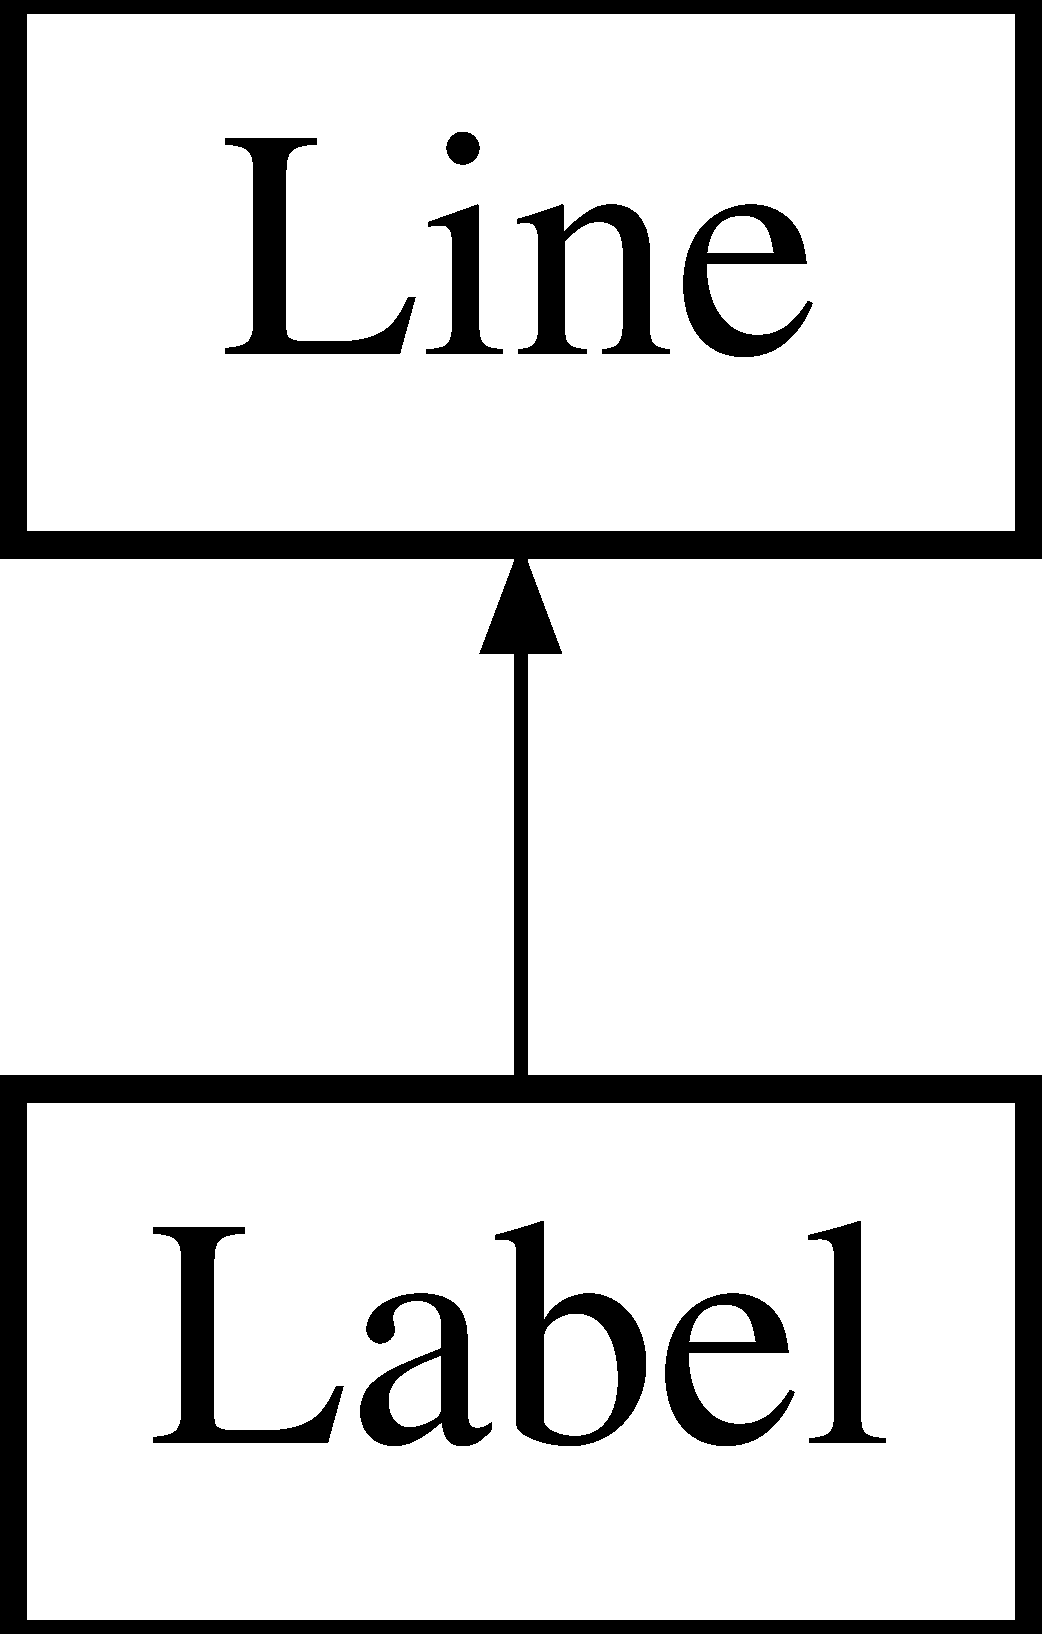
\includegraphics[height=2.000000cm]{classLabel}
\end{center}
\end{figure}
\subsection*{\-Public \-Member \-Functions}
\begin{DoxyCompactItemize}
\item 
\hypertarget{classLabel_a48e774efc0e6e5cd0bf63a94527add17}{\hyperlink{classLabel_a48e774efc0e6e5cd0bf63a94527add17}{\-Label} (string)}\label{classLabel_a48e774efc0e6e5cd0bf63a94527add17}

\begin{DoxyCompactList}\small\item\em \-Constructor of the \hyperlink{classLabel}{\-Label}. \end{DoxyCompactList}\item 
\hypertarget{classLabel_ae0405d591a2ff63c03b104435e2a3066}{virtual \hyperlink{classLabel_ae0405d591a2ff63c03b104435e2a3066}{$\sim$\-Label} ()}\label{classLabel_ae0405d591a2ff63c03b104435e2a3066}

\begin{DoxyCompactList}\small\item\em \-Destructor of the \hyperlink{classLabel}{\-Label}. \end{DoxyCompactList}\item 
\hypertarget{classLabel_afc727d8ae97b32660faf703b30edc77e}{virtual t\-\_\-\-Line \hyperlink{classLabel_afc727d8ae97b32660faf703b30edc77e}{type\-\_\-line} ()}\label{classLabel_afc727d8ae97b32660faf703b30edc77e}

\begin{DoxyCompactList}\small\item\em get the type of the line \end{DoxyCompactList}\item 
\hypertarget{classLabel_a6df2e96366cc459a6a8fa9642a6e69b6}{virtual string \hyperlink{classLabel_a6df2e96366cc459a6a8fa9642a6e69b6}{to\-\_\-string} ()}\label{classLabel_a6df2e96366cc459a6a8fa9642a6e69b6}

\begin{DoxyCompactList}\small\item\em get the string of \hyperlink{classLabel}{\-Label} \end{DoxyCompactList}\item 
\hypertarget{classLabel_a8d48d53b6eb2c6024b7da507bfa5d00b}{virtual string \hyperlink{classLabel_a8d48d53b6eb2c6024b7da507bfa5d00b}{get\-\_\-content} ()}\label{classLabel_a8d48d53b6eb2c6024b7da507bfa5d00b}

\begin{DoxyCompactList}\small\item\em get the string of the \hyperlink{classLabel}{\-Label} \end{DoxyCompactList}\item 
\hypertarget{classLabel_a16f1db5a51a093f3963a2d902bce845f}{virtual void \hyperlink{classLabel_a16f1db5a51a093f3963a2d902bce845f}{set\-\_\-content} (string)}\label{classLabel_a16f1db5a51a093f3963a2d902bce845f}

\begin{DoxyCompactList}\small\item\em set the string of the \hyperlink{classLabel}{\-Label} \end{DoxyCompactList}\item 
\hypertarget{classLabel_af123355b73ac457171c3118052d145ac}{virtual t\-\_\-\-Inst \hyperlink{classLabel_af123355b73ac457171c3118052d145ac}{get\-\_\-type} ()}\label{classLabel_af123355b73ac457171c3118052d145ac}

\begin{DoxyCompactList}\small\item\em return the type of the instruction \end{DoxyCompactList}\end{DoxyCompactItemize}


\subsection{\-Detailed \-Description}
class representing an \hyperlink{classLabel}{\-Label} herited by \hyperlink{classLine}{\-Line} 

\-The documentation for this class was generated from the following file\-:\begin{DoxyCompactItemize}
\item 
\hyperlink{Label_8h}{\-Label.\-h}\end{DoxyCompactItemize}

\hypertarget{classLine}{\section{\-Line \-Class \-Reference}
\label{classLine}\index{\-Line@{\-Line}}
}


\-Abstract class representing an \hyperlink{classLine}{\-Line}.  




{\ttfamily \#include $<$\-Line.\-h$>$}

\-Inheritance diagram for \-Line\-:\begin{figure}[H]
\begin{center}
\leavevmode
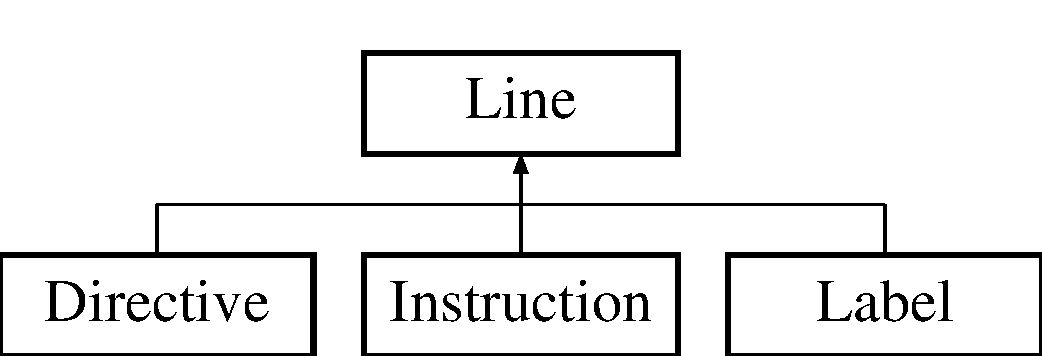
\includegraphics[height=2.000000cm]{classLine}
\end{center}
\end{figure}
\subsection*{\-Public \-Member \-Functions}
\begin{DoxyCompactItemize}
\item 
\hypertarget{classLine_a4a95bafcefa28672b3999deb011b9e50}{virtual \hyperlink{classLine_a4a95bafcefa28672b3999deb011b9e50}{$\sim$\-Line} ()}\label{classLine_a4a95bafcefa28672b3999deb011b9e50}

\begin{DoxyCompactList}\small\item\em \-Virtual destructor. \end{DoxyCompactList}\item 
\hypertarget{classLine_aa7f74673c9c3a7423a513a5fb64bf825}{virtual string \hyperlink{classLine_aa7f74673c9c3a7423a513a5fb64bf825}{get\-\_\-content} ()=0}\label{classLine_aa7f74673c9c3a7423a513a5fb64bf825}

\begin{DoxyCompactList}\small\item\em get the string of the line virtual getter \end{DoxyCompactList}\item 
\hypertarget{classLine_afa27867ffd08e6915d9e791d2ed0b448}{virtual void \hyperlink{classLine_afa27867ffd08e6915d9e791d2ed0b448}{set\-\_\-content} (string)=0}\label{classLine_afa27867ffd08e6915d9e791d2ed0b448}

\begin{DoxyCompactList}\small\item\em set the string of the line virtual setter \end{DoxyCompactList}\item 
\hypertarget{classLine_a0cc2cdd9bc04649adebd1ff9b753bc85}{virtual t\-\_\-\-Line \hyperlink{classLine_a0cc2cdd9bc04649adebd1ff9b753bc85}{type\-\_\-line} ()=0}\label{classLine_a0cc2cdd9bc04649adebd1ff9b753bc85}

\begin{DoxyCompactList}\small\item\em get the type of the line virtual accessor of the type \end{DoxyCompactList}\item 
virtual string \hyperlink{classLine_a477523118f17d72f58f2912b391afc73}{to\-\_\-string} ()=0
\begin{DoxyCompactList}\small\item\em get the name string accessor of the type line \end{DoxyCompactList}\item 
\hypertarget{classLine_a679ddcc8a7d6a634218f177b4d602bd5}{virtual t\-\_\-\-Inst \hyperlink{classLine_a679ddcc8a7d6a634218f177b4d602bd5}{get\-\_\-type} ()=0}\label{classLine_a679ddcc8a7d6a634218f177b4d602bd5}

\begin{DoxyCompactList}\small\item\em return the type of the instruction \end{DoxyCompactList}\item 
\hypertarget{classLine_a57e724949fa0828dfdd2a1bb0f7db8d0}{bool \hyperlink{classLine_a57e724949fa0828dfdd2a1bb0f7db8d0}{is\-Inst} ()}\label{classLine_a57e724949fa0828dfdd2a1bb0f7db8d0}

\begin{DoxyCompactList}\small\item\em tests if the line is an instruction \end{DoxyCompactList}\item 
\hypertarget{classLine_a8323f3df960924826199bd607198ac7f}{bool \hyperlink{classLine_a8323f3df960924826199bd607198ac7f}{is\-Label} ()}\label{classLine_a8323f3df960924826199bd607198ac7f}

\begin{DoxyCompactList}\small\item\em tests if the line is a label \end{DoxyCompactList}\item 
\hypertarget{classLine_ad014e40a75c8a04e6a091ae4110579bc}{bool \hyperlink{classLine_ad014e40a75c8a04e6a091ae4110579bc}{is\-Directive} ()}\label{classLine_ad014e40a75c8a04e6a091ae4110579bc}

\begin{DoxyCompactList}\small\item\em tests if the line is a directive \end{DoxyCompactList}\end{DoxyCompactItemize}
\subsection*{\-Protected \-Attributes}
\begin{DoxyCompactItemize}
\item 
\hypertarget{classLine_a41059923f5c8e5a0f4f44d84bd8762aa}{string {\bfseries \-\_\-line}}\label{classLine_a41059923f5c8e5a0f4f44d84bd8762aa}

\end{DoxyCompactItemize}


\subsection{\-Detailed \-Description}
\-Abstract class representing an \hyperlink{classLine}{\-Line}. 

\subsection{\-Member \-Function \-Documentation}
\hypertarget{classLine_a477523118f17d72f58f2912b391afc73}{\index{\-Line@{\-Line}!to\-\_\-string@{to\-\_\-string}}
\index{to\-\_\-string@{to\-\_\-string}!Line@{\-Line}}
\subsubsection[{to\-\_\-string}]{\setlength{\rightskip}{0pt plus 5cm}virtual string {\bf \-Line\-::to\-\_\-string} (
\begin{DoxyParamCaption}
{}
\end{DoxyParamCaption}
)\hspace{0.3cm}{\ttfamily  \mbox{[}pure virtual\mbox{]}}}}\label{classLine_a477523118f17d72f58f2912b391afc73}


get the name string accessor of the type line 



\-Implemented in \hyperlink{classInstruction_aed87de5e9259f4f15dc885425528f1fe}{\-Instruction}, \hyperlink{classDirective_a2fd56d5580ad7a993782649d7867732f}{\-Directive}, and \hyperlink{classLabel_a6df2e96366cc459a6a8fa9642a6e69b6}{\-Label}.



\-The documentation for this class was generated from the following file\-:\begin{DoxyCompactItemize}
\item 
\hyperlink{Line_8h}{\-Line.\-h}\end{DoxyCompactItemize}

\hypertarget{classNode}{\section{\-Node \-Class \-Reference}
\label{classNode}\index{\-Node@{\-Node}}
}


class representing a \hyperlink{classNode}{\-Node} in list  




{\ttfamily \#include $<$\-Node.\-h$>$}

\subsection*{\-Public \-Member \-Functions}
\begin{DoxyCompactItemize}
\item 
\hypertarget{classNode_a38b4c6850bd8b7f57986ab2131b09918}{\hyperlink{classNode_a38b4c6850bd8b7f57986ab2131b09918}{\-Node} (\hyperlink{classLine}{\-Line} $\ast$content)}\label{classNode_a38b4c6850bd8b7f57986ab2131b09918}

\begin{DoxyCompactList}\small\item\em \hyperlink{classNode}{\-Node} constructor. \end{DoxyCompactList}\item 
\hypertarget{classNode_aa0840c3cb5c7159be6d992adecd2097c}{\hyperlink{classNode_aa0840c3cb5c7159be6d992adecd2097c}{$\sim$\-Node} ()}\label{classNode_aa0840c3cb5c7159be6d992adecd2097c}

\begin{DoxyCompactList}\small\item\em \hyperlink{classNode}{\-Node} destructor. \end{DoxyCompactList}\item 
\hypertarget{classNode_a815c897407e2c039c4d86ef42848d8e5}{\hyperlink{classNode}{\-Node} $\ast$ \hyperlink{classNode_a815c897407e2c039c4d86ef42848d8e5}{get\-\_\-next} ()}\label{classNode_a815c897407e2c039c4d86ef42848d8e5}

\begin{DoxyCompactList}\small\item\em get the next node \end{DoxyCompactList}\item 
\hypertarget{classNode_afdf4d8e60306222a592c1403410c176f}{void \hyperlink{classNode_afdf4d8e60306222a592c1403410c176f}{set\-\_\-next} (\hyperlink{classNode}{\-Node} $\ast$)}\label{classNode_afdf4d8e60306222a592c1403410c176f}

\begin{DoxyCompactList}\small\item\em set the next node \end{DoxyCompactList}\item 
\hypertarget{classNode_ae1f2f87a25c263e385f435059516d0df}{\hyperlink{classNode}{\-Node} $\ast$ \hyperlink{classNode_ae1f2f87a25c263e385f435059516d0df}{get\-\_\-prev} ()}\label{classNode_ae1f2f87a25c263e385f435059516d0df}

\begin{DoxyCompactList}\small\item\em get the previous node \end{DoxyCompactList}\item 
\hypertarget{classNode_ae956250c849d3886566229dc7264e797}{void \hyperlink{classNode_ae956250c849d3886566229dc7264e797}{set\-\_\-prev} (\hyperlink{classNode}{\-Node} $\ast$)}\label{classNode_ae956250c849d3886566229dc7264e797}

\begin{DoxyCompactList}\small\item\em set the previous node \end{DoxyCompactList}\item 
\hypertarget{classNode_a148767567f75e6d3e5e8f8ff9e438336}{\hyperlink{classLine}{\-Line} $\ast$ \hyperlink{classNode_a148767567f75e6d3e5e8f8ff9e438336}{get\-\_\-line} ()}\label{classNode_a148767567f75e6d3e5e8f8ff9e438336}

\begin{DoxyCompactList}\small\item\em get the current line \end{DoxyCompactList}\item 
\hypertarget{classNode_acb0fcb0970c2e2efd9ec90133ea8d236}{void \hyperlink{classNode_acb0fcb0970c2e2efd9ec90133ea8d236}{set\-\_\-line} (\hyperlink{classLine}{\-Line} $\ast$newline)}\label{classNode_acb0fcb0970c2e2efd9ec90133ea8d236}

\begin{DoxyCompactList}\small\item\em set the current line \end{DoxyCompactList}\item 
\hypertarget{classNode_a97c6b9e99919926b82b33444883754f1}{string \hyperlink{classNode_a97c6b9e99919926b82b33444883754f1}{get\-\_\-line\-Content} ()}\label{classNode_a97c6b9e99919926b82b33444883754f1}

\begin{DoxyCompactList}\small\item\em get the content of the line \end{DoxyCompactList}\end{DoxyCompactItemize}


\subsection{\-Detailed \-Description}
class representing a \hyperlink{classNode}{\-Node} in list 

\-The documentation for this class was generated from the following file\-:\begin{DoxyCompactItemize}
\item 
\hyperlink{Node_8h}{\-Node.\-h}\end{DoxyCompactItemize}

\hypertarget{classNode__dfg}{\section{\-Node\-\_\-dfg \-Class \-Reference}
\label{classNode__dfg}\index{\-Node\-\_\-dfg@{\-Node\-\_\-dfg}}
}


class representing a node of data flow graph  




{\ttfamily \#include $<$\-Node\-\_\-dfg.\-h$>$}

\subsection*{\-Public \-Member \-Functions}
\begin{DoxyCompactItemize}
\item 
\hypertarget{classNode__dfg_ac9b79961aaadf29eecd03b227b4c0875}{\hyperlink{classNode__dfg_ac9b79961aaadf29eecd03b227b4c0875}{\-Node\-\_\-dfg} (\hyperlink{classInstruction}{\-Instruction} $\ast$)}\label{classNode__dfg_ac9b79961aaadf29eecd03b227b4c0875}

\begin{DoxyCompactList}\small\item\em \-Constructor of \hyperlink{classNode__dfg}{\-Node\-\_\-dfg}. \end{DoxyCompactList}\item 
\hypertarget{classNode__dfg_a0a2a7c4634ad6802e7c69ab0d95957fa}{\hyperlink{classNode__dfg_a0a2a7c4634ad6802e7c69ab0d95957fa}{$\sim$\-Node\-\_\-dfg} ()}\label{classNode__dfg_a0a2a7c4634ad6802e7c69ab0d95957fa}

\begin{DoxyCompactList}\small\item\em \-Destructor of \hyperlink{classNode__dfg}{\-Node\-\_\-dfg}. \end{DoxyCompactList}\item 
\hypertarget{classNode__dfg_adc4a8e37604e57eec03fecaaca094fb5}{\hyperlink{structArc__t}{\-Arc\-\_\-t} $\ast$ \hyperlink{classNode__dfg_adc4a8e37604e57eec03fecaaca094fb5}{get\-\_\-arc} (int i)}\label{classNode__dfg_adc4a8e37604e57eec03fecaaca094fb5}

\begin{DoxyCompactList}\small\item\em get the ith arc of the arc list \end{DoxyCompactList}\item 
\hypertarget{classNode__dfg_a6ebd568efb70f729f6e355cdd46a5185}{list$<$ \hyperlink{structArc__t}{\-Arc\-\_\-t} $\ast$ $>$\-::iterator {\bfseries arcs\-\_\-begin} ()}\label{classNode__dfg_a6ebd568efb70f729f6e355cdd46a5185}

\item 
\hypertarget{classNode__dfg_a5a49217bcb16aaf7e94e4e156d9a9d53}{list$<$ \hyperlink{structArc__t}{\-Arc\-\_\-t} $\ast$ $>$\-::iterator {\bfseries arcs\-\_\-end} ()}\label{classNode__dfg_a5a49217bcb16aaf7e94e4e156d9a9d53}

\item 
\hypertarget{classNode__dfg_a85d42a5cc1d6feacf403a8569a813074}{int \hyperlink{classNode__dfg_a85d42a5cc1d6feacf403a8569a813074}{get\-\_\-nb\-\_\-arcs} ()}\label{classNode__dfg_a85d42a5cc1d6feacf403a8569a813074}

\begin{DoxyCompactList}\small\item\em get the number of arcs \end{DoxyCompactList}\item 
\hypertarget{classNode__dfg_a8f20c21a0ffb2e224cc426148362c249}{\hyperlink{classInstruction}{\-Instruction} $\ast$ \hyperlink{classNode__dfg_a8f20c21a0ffb2e224cc426148362c249}{get\-\_\-instruction} ()}\label{classNode__dfg_a8f20c21a0ffb2e224cc426148362c249}

\begin{DoxyCompactList}\small\item\em get the \hyperlink{classInstruction}{\-Instruction} \end{DoxyCompactList}\item 
\hypertarget{classNode__dfg_a2fa3283cfba68ea72294810c6e39be61}{void \hyperlink{classNode__dfg_a2fa3283cfba68ea72294810c6e39be61}{add\-\_\-arc} (\hyperlink{structArc__t}{\-Arc\-\_\-t} $\ast$)}\label{classNode__dfg_a2fa3283cfba68ea72294810c6e39be61}

\begin{DoxyCompactList}\small\item\em add an arc to the arc list \end{DoxyCompactList}\item 
\hypertarget{classNode__dfg_a8cc89b32dbe15bcf399725955a643551}{void {\bfseries add\-\_\-predecesseur} (\hyperlink{classNode__dfg}{\-Node\-\_\-dfg} $\ast$)}\label{classNode__dfg_a8cc89b32dbe15bcf399725955a643551}

\item 
\hypertarget{classNode__dfg_adef5e6e3362133f6adb38d404c8d8cf6}{int {\bfseries nb\-\_\-preds} ()}\label{classNode__dfg_adef5e6e3362133f6adb38d404c8d8cf6}

\item 
\hypertarget{classNode__dfg_a769af0d7836679d6ee9abcc55d399887}{list$<$ \hyperlink{classNode__dfg}{\-Node\-\_\-dfg} $\ast$ $>$\-::iterator {\bfseries pred\-\_\-begin} ()}\label{classNode__dfg_a769af0d7836679d6ee9abcc55d399887}

\item 
\hypertarget{classNode__dfg_a86fc141e0697ae944900625212579957}{list$<$ \hyperlink{classNode__dfg}{\-Node\-\_\-dfg} $\ast$ $>$\-::iterator {\bfseries pred\-\_\-end} ()}\label{classNode__dfg_a86fc141e0697ae944900625212579957}

\item 
\hypertarget{classNode__dfg_a83747917d9c87b11633779731bcda162}{void \hyperlink{classNode__dfg_a83747917d9c87b11633779731bcda162}{set\-\_\-instruction} (\hyperlink{classInstruction}{\-Instruction} $\ast$)}\label{classNode__dfg_a83747917d9c87b11633779731bcda162}

\begin{DoxyCompactList}\small\item\em set the \hyperlink{classInstruction}{\-Instruction} \end{DoxyCompactList}\item 
\hypertarget{classNode__dfg_af23f48b1521a90178cc5c9a59da3ab3c}{void \hyperlink{classNode__dfg_af23f48b1521a90178cc5c9a59da3ab3c}{set\-\_\-weight} (int)}\label{classNode__dfg_af23f48b1521a90178cc5c9a59da3ab3c}

\begin{DoxyCompactList}\small\item\em set the weight \end{DoxyCompactList}\item 
\hypertarget{classNode__dfg_a561e80f51cb9a71b22f22e8d2e6685de}{int \hyperlink{classNode__dfg_a561e80f51cb9a71b22f22e8d2e6685de}{get\-\_\-weight} ()}\label{classNode__dfg_a561e80f51cb9a71b22f22e8d2e6685de}

\begin{DoxyCompactList}\small\item\em get the weight \end{DoxyCompactList}\item 
\hypertarget{classNode__dfg_a9aa775f727e6c542cd714894219046f3}{void \hyperlink{classNode__dfg_a9aa775f727e6c542cd714894219046f3}{set\-\_\-nb\-\_\-descendant} (int)}\label{classNode__dfg_a9aa775f727e6c542cd714894219046f3}

\begin{DoxyCompactList}\small\item\em set the number of descendant \end{DoxyCompactList}\item 
\hypertarget{classNode__dfg_a9baa0a6be056b7d1ee290c404f2216f5}{int \hyperlink{classNode__dfg_a9baa0a6be056b7d1ee290c404f2216f5}{get\-\_\-nb\-\_\-descendant} ()}\label{classNode__dfg_a9baa0a6be056b7d1ee290c404f2216f5}

\begin{DoxyCompactList}\small\item\em get the number of descendant \end{DoxyCompactList}\item 
\hypertarget{classNode__dfg_ad9fe88cf90fa2282806edbc64f51331e}{void \hyperlink{classNode__dfg_ad9fe88cf90fa2282806edbc64f51331e}{set\-\_\-tready} (int t)}\label{classNode__dfg_ad9fe88cf90fa2282806edbc64f51331e}

\begin{DoxyCompactList}\small\item\em set tready to t \end{DoxyCompactList}\item 
\hypertarget{classNode__dfg_a05e8db316dd2db8b0946167763585c7b}{int \hyperlink{classNode__dfg_a05e8db316dd2db8b0946167763585c7b}{get\-\_\-tready} ()}\label{classNode__dfg_a05e8db316dd2db8b0946167763585c7b}

\begin{DoxyCompactList}\small\item\em returns tready \end{DoxyCompactList}\item 
\hypertarget{classNode__dfg_a07364912fb02e421e79597f91cf5140f}{void {\bfseries set\-\_\-traitee} (int num)}\label{classNode__dfg_a07364912fb02e421e79597f91cf5140f}

\item 
\hypertarget{classNode__dfg_a1b0ec3773d7eaaaf44f40b91cc6b4358}{int {\bfseries get\-\_\-traitee} ()}\label{classNode__dfg_a1b0ec3773d7eaaaf44f40b91cc6b4358}

\end{DoxyCompactItemize}


\subsection{\-Detailed \-Description}
class representing a node of data flow graph 

\-The documentation for this class was generated from the following file\-:\begin{DoxyCompactItemize}
\item 
\hyperlink{Node__dfg_8h}{\-Node\-\_\-dfg.\-h}\end{DoxyCompactItemize}

\hypertarget{classOperand}{\section{\-Operand \-Class \-Reference}
\label{classOperand}\index{\-Operand@{\-Operand}}
}


\-Abstract class representing an operand.  




{\ttfamily \#include $<$\-Operand.\-h$>$}

\-Inheritance diagram for \-Operand\-:\begin{figure}[H]
\begin{center}
\leavevmode
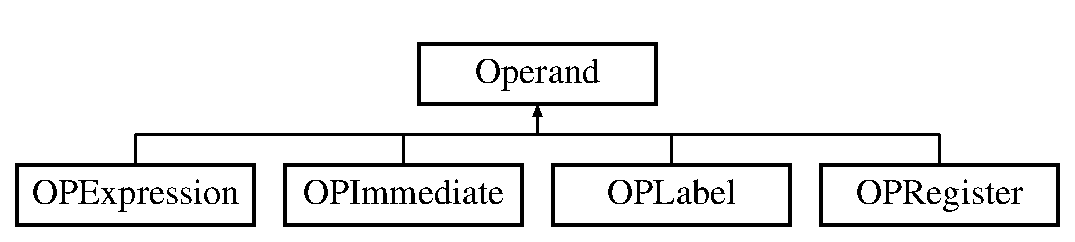
\includegraphics[height=2.000000cm]{classOperand}
\end{center}
\end{figure}
\subsection*{\-Public \-Member \-Functions}
\begin{DoxyCompactItemize}
\item 
\hypertarget{classOperand_aa6ef1ffa183381edb413f9b93782a67b}{virtual \hyperlink{classOperand_aa6ef1ffa183381edb413f9b93782a67b}{$\sim$\-Operand} ()}\label{classOperand_aa6ef1ffa183381edb413f9b93782a67b}

\begin{DoxyCompactList}\small\item\em \-Virtual destructor. \end{DoxyCompactList}\item 
\hypertarget{classOperand_a2bf3ad8b34d39cb35ff743ffcc0f4675}{virtual string \hyperlink{classOperand_a2bf3ad8b34d39cb35ff743ffcc0f4675}{get\-\_\-op} ()=0}\label{classOperand_a2bf3ad8b34d39cb35ff743ffcc0f4675}

\begin{DoxyCompactList}\small\item\em \-Get the operand value virtual accessor of the operand. \end{DoxyCompactList}\item 
\hypertarget{classOperand_a0895c39d7b97ea56f074d242e8232c78}{virtual void \hyperlink{classOperand_a0895c39d7b97ea56f074d242e8232c78}{set\-\_\-op} (string)=0}\label{classOperand_a0895c39d7b97ea56f074d242e8232c78}

\begin{DoxyCompactList}\small\item\em set the operand value virtual setter of the operand \end{DoxyCompactList}\item 
virtual t\-\_\-\-Op\-Type \hyperlink{classOperand_afd469e305a467e2574f34ac9bd6c62b0}{get\-\_\-op\-\_\-type} ()=0
\begin{DoxyCompactList}\small\item\em get the operator type virtual accessor of accessor \end{DoxyCompactList}\item 
virtual string \hyperlink{classOperand_a28aed96d5fafee66be81c30c1435ad00}{to\-\_\-string} ()=0
\begin{DoxyCompactList}\small\item\em virtual tostring \end{DoxyCompactList}\end{DoxyCompactItemize}
\subsection*{\-Protected \-Attributes}
\begin{DoxyCompactItemize}
\item 
\hypertarget{classOperand_af70a183445064a0106d41dfeea681790}{string {\bfseries \-\_\-oper}}\label{classOperand_af70a183445064a0106d41dfeea681790}

\end{DoxyCompactItemize}


\subsection{\-Detailed \-Description}
\-Abstract class representing an operand. 

\subsection{\-Member \-Function \-Documentation}
\hypertarget{classOperand_afd469e305a467e2574f34ac9bd6c62b0}{\index{\-Operand@{\-Operand}!get\-\_\-op\-\_\-type@{get\-\_\-op\-\_\-type}}
\index{get\-\_\-op\-\_\-type@{get\-\_\-op\-\_\-type}!Operand@{\-Operand}}
\subsubsection[{get\-\_\-op\-\_\-type}]{\setlength{\rightskip}{0pt plus 5cm}virtual t\-\_\-\-Op\-Type {\bf \-Operand\-::get\-\_\-op\-\_\-type} (
\begin{DoxyParamCaption}
{}
\end{DoxyParamCaption}
)\hspace{0.3cm}{\ttfamily  \mbox{[}pure virtual\mbox{]}}}}\label{classOperand_afd469e305a467e2574f34ac9bd6c62b0}


get the operator type virtual accessor of accessor 

\begin{DoxyReturn}{\-Returns}
return the \hyperlink{classOperand}{\-Operand} type as enum 
\end{DoxyReturn}


\-Implemented in \hyperlink{classOPRegister_a1be03d6e6422510a1fd12d1f13dfd601}{\-O\-P\-Register}, \hyperlink{classOPImmediate_aed01353798ae57936a9f77dd05eafa88}{\-O\-P\-Immediate}, \hyperlink{classOPExpression_a06f8902130516437d5d93c43a5efcbd2}{\-O\-P\-Expression}, and \hyperlink{classOPLabel_a1a6ec701c549a6475d44ffcced1c23b5}{\-O\-P\-Label}.

\hypertarget{classOperand_a28aed96d5fafee66be81c30c1435ad00}{\index{\-Operand@{\-Operand}!to\-\_\-string@{to\-\_\-string}}
\index{to\-\_\-string@{to\-\_\-string}!Operand@{\-Operand}}
\subsubsection[{to\-\_\-string}]{\setlength{\rightskip}{0pt plus 5cm}virtual string {\bf \-Operand\-::to\-\_\-string} (
\begin{DoxyParamCaption}
{}
\end{DoxyParamCaption}
)\hspace{0.3cm}{\ttfamily  \mbox{[}pure virtual\mbox{]}}}}\label{classOperand_a28aed96d5fafee66be81c30c1435ad00}


virtual tostring 

\begin{DoxyReturn}{\-Returns}
return the \-Object as string 
\end{DoxyReturn}


\-Implemented in \hyperlink{classOPRegister_a9f55bdff75224fb18973a9e913a4022f}{\-O\-P\-Register}, \hyperlink{classOPImmediate_a12bc613de3bff73ead8632dafd8050a0}{\-O\-P\-Immediate}, \hyperlink{classOPExpression_a0a6ee03eb083791028eeae021f4ff47b}{\-O\-P\-Expression}, and \hyperlink{classOPLabel_a51c4e8f45422f03edcb71d472cf5e973}{\-O\-P\-Label}.



\-The documentation for this class was generated from the following file\-:\begin{DoxyCompactItemize}
\item 
\hyperlink{Operand_8h}{\-Operand.\-h}\end{DoxyCompactItemize}

\hypertarget{classOPExpression}{\section{\-O\-P\-Expression \-Class \-Reference}
\label{classOPExpression}\index{\-O\-P\-Expression@{\-O\-P\-Expression}}
}


class representing an expression herited by \hyperlink{classOperand}{\-Operand}  




{\ttfamily \#include $<$\-O\-P\-Expression.\-h$>$}

\-Inheritance diagram for \-O\-P\-Expression\-:\begin{figure}[H]
\begin{center}
\leavevmode
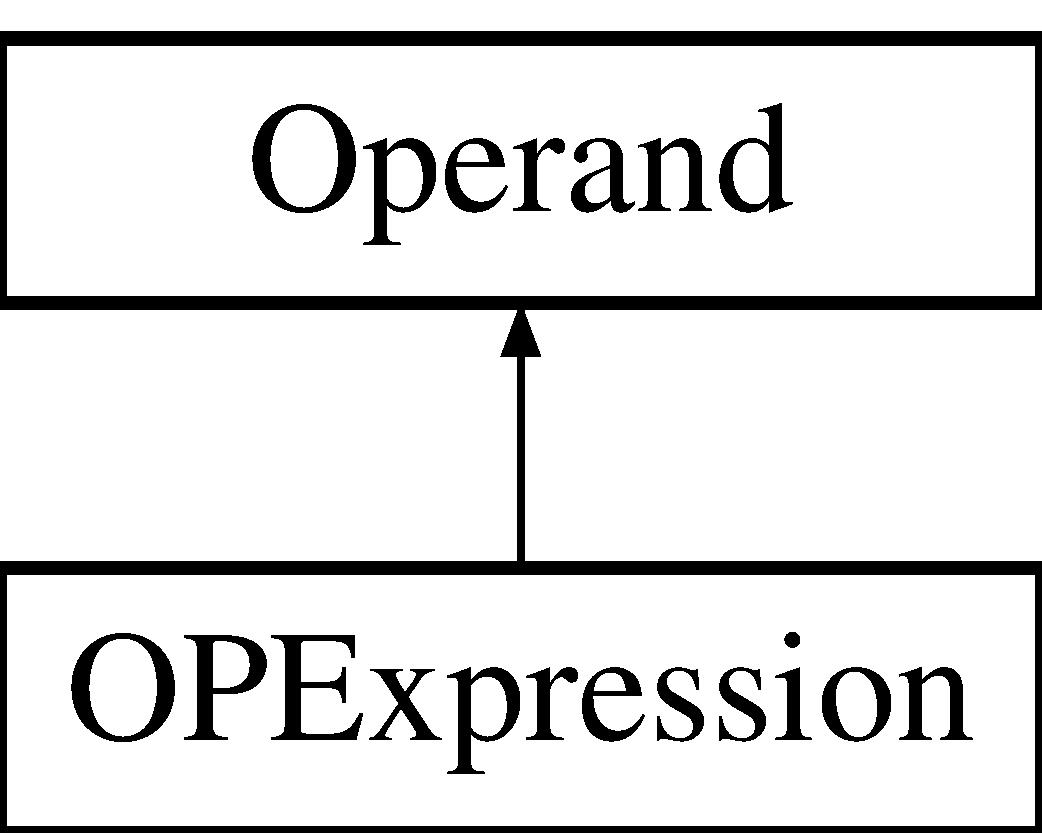
\includegraphics[height=2.000000cm]{classOPExpression}
\end{center}
\end{figure}
\subsection*{\-Public \-Member \-Functions}
\begin{DoxyCompactItemize}
\item 
\hypertarget{classOPExpression_a5784034daef8568869fe0bb5ecfbcdcf}{\hyperlink{classOPExpression_a5784034daef8568869fe0bb5ecfbcdcf}{\-O\-P\-Expression} (string)}\label{classOPExpression_a5784034daef8568869fe0bb5ecfbcdcf}

\begin{DoxyCompactList}\small\item\em \-Constructor of the \-Expression class. \end{DoxyCompactList}\item 
\hypertarget{classOPExpression_a5ea892d89208ccb593510ee63ef42a19}{virtual \hyperlink{classOPExpression_a5ea892d89208ccb593510ee63ef42a19}{$\sim$\-O\-P\-Expression} ()}\label{classOPExpression_a5ea892d89208ccb593510ee63ef42a19}

\begin{DoxyCompactList}\small\item\em \-Destructor of the \-Expression class. \end{DoxyCompactList}\item 
virtual string \hyperlink{classOPExpression_acf86deca614626b803bc3c29facbefef}{get\-\_\-op} ()
\begin{DoxyCompactList}\small\item\em \-Get the operand value. \end{DoxyCompactList}\item 
virtual t\-\_\-\-Op\-Type \hyperlink{classOPExpression_a06f8902130516437d5d93c43a5efcbd2}{get\-\_\-op\-\_\-type} ()
\begin{DoxyCompactList}\small\item\em get the operator type \end{DoxyCompactList}\item 
virtual string \hyperlink{classOPExpression_a0a6ee03eb083791028eeae021f4ff47b}{to\-\_\-string} ()
\begin{DoxyCompactList}\small\item\em tostring \end{DoxyCompactList}\item 
\hypertarget{classOPExpression_a3cfeacf4f76611d374be3caa9de80a05}{virtual void \hyperlink{classOPExpression_a3cfeacf4f76611d374be3caa9de80a05}{set\-\_\-op} (string)}\label{classOPExpression_a3cfeacf4f76611d374be3caa9de80a05}

\begin{DoxyCompactList}\small\item\em set the operand value setter of the operand \end{DoxyCompactList}\end{DoxyCompactItemize}


\subsection{\-Detailed \-Description}
class representing an expression herited by \hyperlink{classOperand}{\-Operand} 

\subsection{\-Member \-Function \-Documentation}
\hypertarget{classOPExpression_acf86deca614626b803bc3c29facbefef}{\index{\-O\-P\-Expression@{\-O\-P\-Expression}!get\-\_\-op@{get\-\_\-op}}
\index{get\-\_\-op@{get\-\_\-op}!OPExpression@{\-O\-P\-Expression}}
\subsubsection[{get\-\_\-op}]{\setlength{\rightskip}{0pt plus 5cm}virtual string {\bf \-O\-P\-Expression\-::get\-\_\-op} (
\begin{DoxyParamCaption}
{}
\end{DoxyParamCaption}
)\hspace{0.3cm}{\ttfamily  \mbox{[}virtual\mbox{]}}}}\label{classOPExpression_acf86deca614626b803bc3c29facbefef}


\-Get the operand value. 

\begin{DoxyReturn}{\-Returns}
return the string of the \-Expression 
\end{DoxyReturn}


\-Implements \hyperlink{classOperand_a2bf3ad8b34d39cb35ff743ffcc0f4675}{\-Operand}.

\hypertarget{classOPExpression_a06f8902130516437d5d93c43a5efcbd2}{\index{\-O\-P\-Expression@{\-O\-P\-Expression}!get\-\_\-op\-\_\-type@{get\-\_\-op\-\_\-type}}
\index{get\-\_\-op\-\_\-type@{get\-\_\-op\-\_\-type}!OPExpression@{\-O\-P\-Expression}}
\subsubsection[{get\-\_\-op\-\_\-type}]{\setlength{\rightskip}{0pt plus 5cm}virtual t\-\_\-\-Op\-Type {\bf \-O\-P\-Expression\-::get\-\_\-op\-\_\-type} (
\begin{DoxyParamCaption}
{}
\end{DoxyParamCaption}
)\hspace{0.3cm}{\ttfamily  \mbox{[}virtual\mbox{]}}}}\label{classOPExpression_a06f8902130516437d5d93c43a5efcbd2}


get the operator type 

\begin{DoxyReturn}{\-Returns}
return the \hyperlink{classOperand}{\-Operand} type as enum 
\end{DoxyReturn}


\-Implements \hyperlink{classOperand_afd469e305a467e2574f34ac9bd6c62b0}{\-Operand}.

\hypertarget{classOPExpression_a0a6ee03eb083791028eeae021f4ff47b}{\index{\-O\-P\-Expression@{\-O\-P\-Expression}!to\-\_\-string@{to\-\_\-string}}
\index{to\-\_\-string@{to\-\_\-string}!OPExpression@{\-O\-P\-Expression}}
\subsubsection[{to\-\_\-string}]{\setlength{\rightskip}{0pt plus 5cm}virtual string {\bf \-O\-P\-Expression\-::to\-\_\-string} (
\begin{DoxyParamCaption}
{}
\end{DoxyParamCaption}
)\hspace{0.3cm}{\ttfamily  \mbox{[}virtual\mbox{]}}}}\label{classOPExpression_a0a6ee03eb083791028eeae021f4ff47b}


tostring 

\begin{DoxyReturn}{\-Returns}
return the \-Object as string 
\end{DoxyReturn}


\-Implements \hyperlink{classOperand_a28aed96d5fafee66be81c30c1435ad00}{\-Operand}.



\-The documentation for this class was generated from the following file\-:\begin{DoxyCompactItemize}
\item 
\hyperlink{OPExpression_8h}{\-O\-P\-Expression.\-h}\end{DoxyCompactItemize}

\hypertarget{classOPImmediate}{\section{\-O\-P\-Immediate \-Class \-Reference}
\label{classOPImmediate}\index{\-O\-P\-Immediate@{\-O\-P\-Immediate}}
}


class representing an \-Immediate herited by \hyperlink{classOperand}{\-Operand}  




{\ttfamily \#include $<$\-O\-P\-Immediate.\-h$>$}

\-Inheritance diagram for \-O\-P\-Immediate\-:\begin{figure}[H]
\begin{center}
\leavevmode
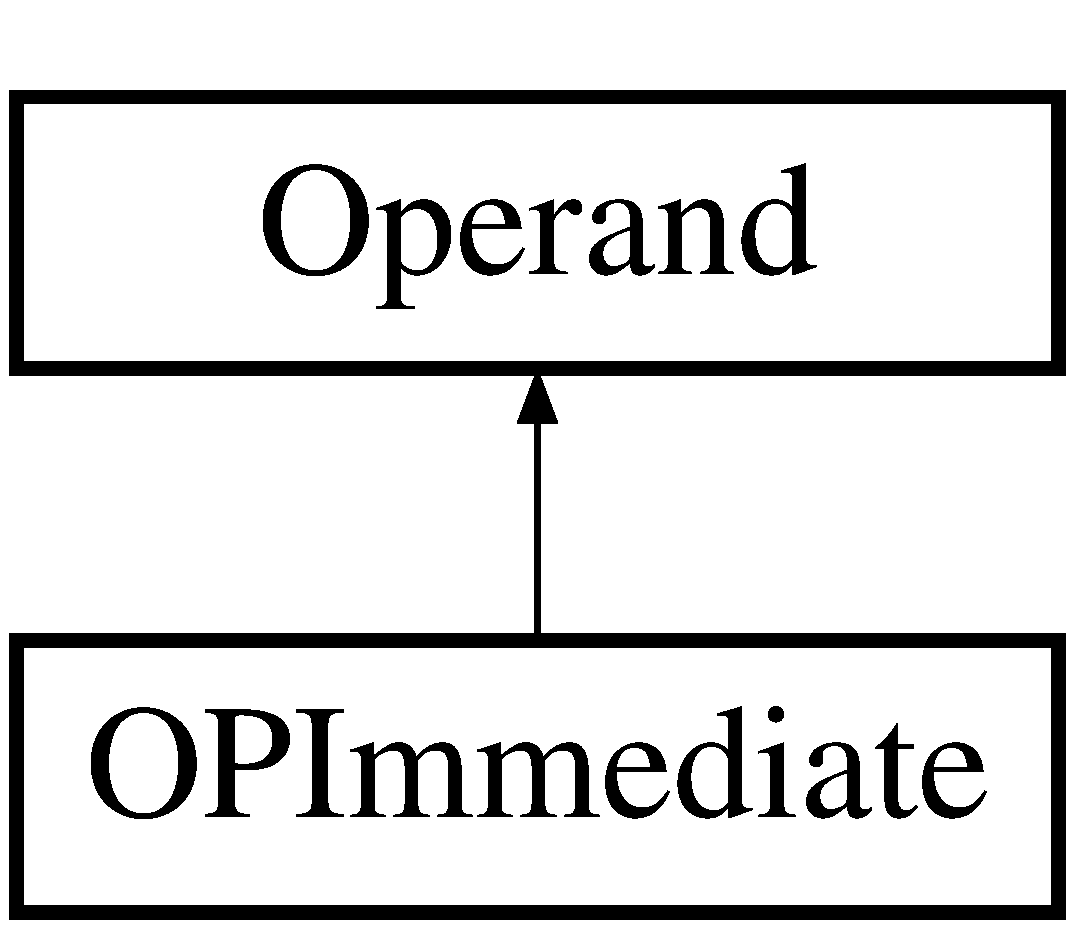
\includegraphics[height=2.000000cm]{classOPImmediate}
\end{center}
\end{figure}
\subsection*{\-Public \-Member \-Functions}
\begin{DoxyCompactItemize}
\item 
\hypertarget{classOPImmediate_ab047dac5f3390947a21e4ab118c05857}{\hyperlink{classOPImmediate_ab047dac5f3390947a21e4ab118c05857}{\-O\-P\-Immediate} (string)}\label{classOPImmediate_ab047dac5f3390947a21e4ab118c05857}

\begin{DoxyCompactList}\small\item\em \-Constructor of the \-Immediate \-Class. \end{DoxyCompactList}\item 
\hypertarget{classOPImmediate_ae940dcf9e9050227a94c759a0cae6861}{\hyperlink{classOPImmediate_ae940dcf9e9050227a94c759a0cae6861}{\-O\-P\-Immediate} (int)}\label{classOPImmediate_ae940dcf9e9050227a94c759a0cae6861}

\begin{DoxyCompactList}\small\item\em \-Constructor of the \-Immediate \-Class. \end{DoxyCompactList}\item 
\hypertarget{classOPImmediate_af7f51ae61e075e02817d6ecd7441408f}{virtual \hyperlink{classOPImmediate_af7f51ae61e075e02817d6ecd7441408f}{$\sim$\-O\-P\-Immediate} ()}\label{classOPImmediate_af7f51ae61e075e02817d6ecd7441408f}

\begin{DoxyCompactList}\small\item\em \-Destructor of the \-Immediate \-Class. \end{DoxyCompactList}\item 
virtual string \hyperlink{classOPImmediate_ad714fb614c0d8f4afa1157a34b2936fd}{get\-\_\-op} ()
\begin{DoxyCompactList}\small\item\em \-Get the string of the operand. \end{DoxyCompactList}\item 
virtual t\-\_\-\-Op\-Type \hyperlink{classOPImmediate_aed01353798ae57936a9f77dd05eafa88}{get\-\_\-op\-\_\-type} ()
\begin{DoxyCompactList}\small\item\em get the operator type \end{DoxyCompactList}\item 
virtual string \hyperlink{classOPImmediate_a12bc613de3bff73ead8632dafd8050a0}{to\-\_\-string} ()
\begin{DoxyCompactList}\small\item\em tostring \end{DoxyCompactList}\item 
\hypertarget{classOPImmediate_ae5d6c30c6bff17de4e7fabb24cf6bf59}{virtual void \hyperlink{classOPImmediate_ae5d6c30c6bff17de4e7fabb24cf6bf59}{set\-\_\-op} (string)}\label{classOPImmediate_ae5d6c30c6bff17de4e7fabb24cf6bf59}

\begin{DoxyCompactList}\small\item\em set the string of the operand setter of the operand \end{DoxyCompactList}\end{DoxyCompactItemize}


\subsection{\-Detailed \-Description}
class representing an \-Immediate herited by \hyperlink{classOperand}{\-Operand} 

\subsection{\-Member \-Function \-Documentation}
\hypertarget{classOPImmediate_ad714fb614c0d8f4afa1157a34b2936fd}{\index{\-O\-P\-Immediate@{\-O\-P\-Immediate}!get\-\_\-op@{get\-\_\-op}}
\index{get\-\_\-op@{get\-\_\-op}!OPImmediate@{\-O\-P\-Immediate}}
\subsubsection[{get\-\_\-op}]{\setlength{\rightskip}{0pt plus 5cm}virtual string {\bf \-O\-P\-Immediate\-::get\-\_\-op} (
\begin{DoxyParamCaption}
{}
\end{DoxyParamCaption}
)\hspace{0.3cm}{\ttfamily  \mbox{[}virtual\mbox{]}}}}\label{classOPImmediate_ad714fb614c0d8f4afa1157a34b2936fd}


\-Get the string of the operand. 

\begin{DoxyReturn}{\-Returns}
return the string of the \-Immediate 
\end{DoxyReturn}


\-Implements \hyperlink{classOperand_a2bf3ad8b34d39cb35ff743ffcc0f4675}{\-Operand}.

\hypertarget{classOPImmediate_aed01353798ae57936a9f77dd05eafa88}{\index{\-O\-P\-Immediate@{\-O\-P\-Immediate}!get\-\_\-op\-\_\-type@{get\-\_\-op\-\_\-type}}
\index{get\-\_\-op\-\_\-type@{get\-\_\-op\-\_\-type}!OPImmediate@{\-O\-P\-Immediate}}
\subsubsection[{get\-\_\-op\-\_\-type}]{\setlength{\rightskip}{0pt plus 5cm}virtual t\-\_\-\-Op\-Type {\bf \-O\-P\-Immediate\-::get\-\_\-op\-\_\-type} (
\begin{DoxyParamCaption}
{}
\end{DoxyParamCaption}
)\hspace{0.3cm}{\ttfamily  \mbox{[}virtual\mbox{]}}}}\label{classOPImmediate_aed01353798ae57936a9f77dd05eafa88}


get the operator type 

\begin{DoxyReturn}{\-Returns}
return the \hyperlink{classOperand}{\-Operand} type as enum 
\end{DoxyReturn}


\-Implements \hyperlink{classOperand_afd469e305a467e2574f34ac9bd6c62b0}{\-Operand}.

\hypertarget{classOPImmediate_a12bc613de3bff73ead8632dafd8050a0}{\index{\-O\-P\-Immediate@{\-O\-P\-Immediate}!to\-\_\-string@{to\-\_\-string}}
\index{to\-\_\-string@{to\-\_\-string}!OPImmediate@{\-O\-P\-Immediate}}
\subsubsection[{to\-\_\-string}]{\setlength{\rightskip}{0pt plus 5cm}virtual string {\bf \-O\-P\-Immediate\-::to\-\_\-string} (
\begin{DoxyParamCaption}
{}
\end{DoxyParamCaption}
)\hspace{0.3cm}{\ttfamily  \mbox{[}virtual\mbox{]}}}}\label{classOPImmediate_a12bc613de3bff73ead8632dafd8050a0}


tostring 

\begin{DoxyReturn}{\-Returns}
return the name of the \-Object as string 
\end{DoxyReturn}


\-Implements \hyperlink{classOperand_a28aed96d5fafee66be81c30c1435ad00}{\-Operand}.



\-The documentation for this class was generated from the following file\-:\begin{DoxyCompactItemize}
\item 
\hyperlink{OPImmediate_8h}{\-O\-P\-Immediate.\-h}\end{DoxyCompactItemize}

\hypertarget{classOPLabel}{\section{\-O\-P\-Label \-Class \-Reference}
\label{classOPLabel}\index{\-O\-P\-Label@{\-O\-P\-Label}}
}


class representing a \hyperlink{classLabel}{\-Label} herited by \hyperlink{classOperand}{\-Operand}  




{\ttfamily \#include $<$\-O\-P\-Label.\-h$>$}

\-Inheritance diagram for \-O\-P\-Label\-:\begin{figure}[H]
\begin{center}
\leavevmode
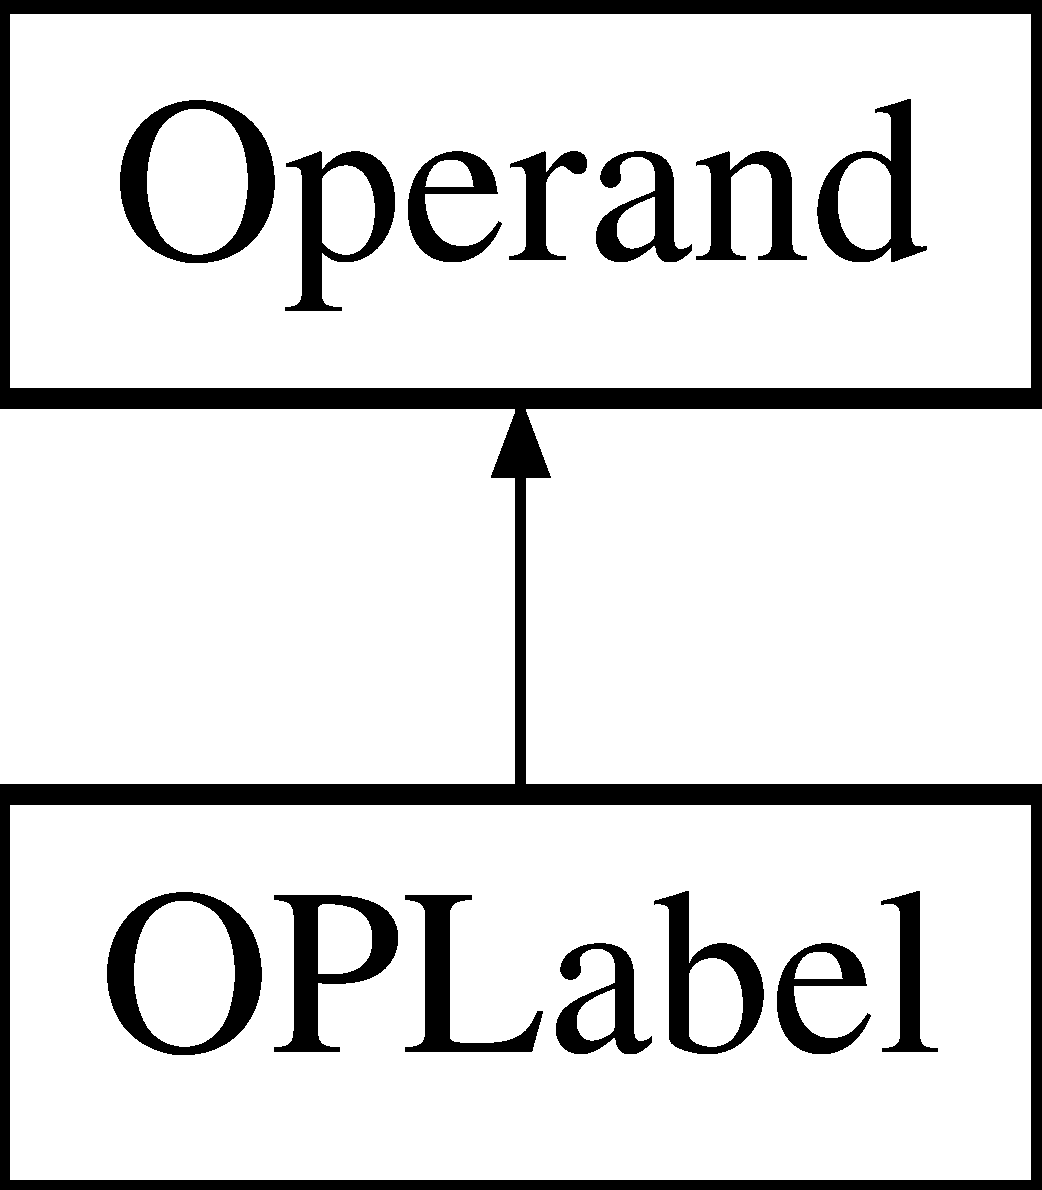
\includegraphics[height=2.000000cm]{classOPLabel}
\end{center}
\end{figure}
\subsection*{\-Public \-Member \-Functions}
\begin{DoxyCompactItemize}
\item 
\hypertarget{classOPLabel_a5405b78894658047362a328e750f88b4}{\hyperlink{classOPLabel_a5405b78894658047362a328e750f88b4}{\-O\-P\-Label} (string)}\label{classOPLabel_a5405b78894658047362a328e750f88b4}

\begin{DoxyCompactList}\small\item\em \-Constructor of the \hyperlink{classLabel}{\-Label} \-Class. \end{DoxyCompactList}\item 
\hypertarget{classOPLabel_ab25553d41606e880a622e09d5c09129d}{virtual \hyperlink{classOPLabel_ab25553d41606e880a622e09d5c09129d}{$\sim$\-O\-P\-Label} ()}\label{classOPLabel_ab25553d41606e880a622e09d5c09129d}

\begin{DoxyCompactList}\small\item\em \-Destructor of the \hyperlink{classLabel}{\-Label} \-Class. \end{DoxyCompactList}\item 
\hypertarget{classOPLabel_a1c933d10a7b2267bae3bea6c385d466f}{virtual string \hyperlink{classOPLabel_a1c933d10a7b2267bae3bea6c385d466f}{get\-\_\-op} ()}\label{classOPLabel_a1c933d10a7b2267bae3bea6c385d466f}

\begin{DoxyCompactList}\small\item\em \-Get the string of the operand accessor of the operand. \end{DoxyCompactList}\item 
virtual t\-\_\-\-Op\-Type \hyperlink{classOPLabel_a1a6ec701c549a6475d44ffcced1c23b5}{get\-\_\-op\-\_\-type} ()
\begin{DoxyCompactList}\small\item\em get the operator type \end{DoxyCompactList}\item 
virtual string \hyperlink{classOPLabel_a51c4e8f45422f03edcb71d472cf5e973}{to\-\_\-string} ()
\begin{DoxyCompactList}\small\item\em tostring \end{DoxyCompactList}\item 
\hypertarget{classOPLabel_a189bec8bcf7300e6e8656ce4bb443995}{virtual void \hyperlink{classOPLabel_a189bec8bcf7300e6e8656ce4bb443995}{set\-\_\-op} (string)}\label{classOPLabel_a189bec8bcf7300e6e8656ce4bb443995}

\begin{DoxyCompactList}\small\item\em set the operand value setter of the operand \end{DoxyCompactList}\end{DoxyCompactItemize}


\subsection{\-Detailed \-Description}
class representing a \hyperlink{classLabel}{\-Label} herited by \hyperlink{classOperand}{\-Operand} 

\subsection{\-Member \-Function \-Documentation}
\hypertarget{classOPLabel_a1a6ec701c549a6475d44ffcced1c23b5}{\index{\-O\-P\-Label@{\-O\-P\-Label}!get\-\_\-op\-\_\-type@{get\-\_\-op\-\_\-type}}
\index{get\-\_\-op\-\_\-type@{get\-\_\-op\-\_\-type}!OPLabel@{\-O\-P\-Label}}
\subsubsection[{get\-\_\-op\-\_\-type}]{\setlength{\rightskip}{0pt plus 5cm}virtual t\-\_\-\-Op\-Type {\bf \-O\-P\-Label\-::get\-\_\-op\-\_\-type} (
\begin{DoxyParamCaption}
{}
\end{DoxyParamCaption}
)\hspace{0.3cm}{\ttfamily  \mbox{[}virtual\mbox{]}}}}\label{classOPLabel_a1a6ec701c549a6475d44ffcced1c23b5}


get the operator type 

\begin{DoxyReturn}{\-Returns}
return the \hyperlink{classOperand}{\-Operand} type as enum 
\end{DoxyReturn}


\-Implements \hyperlink{classOperand_afd469e305a467e2574f34ac9bd6c62b0}{\-Operand}.

\hypertarget{classOPLabel_a51c4e8f45422f03edcb71d472cf5e973}{\index{\-O\-P\-Label@{\-O\-P\-Label}!to\-\_\-string@{to\-\_\-string}}
\index{to\-\_\-string@{to\-\_\-string}!OPLabel@{\-O\-P\-Label}}
\subsubsection[{to\-\_\-string}]{\setlength{\rightskip}{0pt plus 5cm}virtual string {\bf \-O\-P\-Label\-::to\-\_\-string} (
\begin{DoxyParamCaption}
{}
\end{DoxyParamCaption}
)\hspace{0.3cm}{\ttfamily  \mbox{[}virtual\mbox{]}}}}\label{classOPLabel_a51c4e8f45422f03edcb71d472cf5e973}


tostring 

\begin{DoxyReturn}{\-Returns}
return the name of the \-Object as string 
\end{DoxyReturn}


\-Implements \hyperlink{classOperand_a28aed96d5fafee66be81c30c1435ad00}{\-Operand}.



\-The documentation for this class was generated from the following file\-:\begin{DoxyCompactItemize}
\item 
\hyperlink{OPLabel_8h}{\-O\-P\-Label.\-h}\end{DoxyCompactItemize}

\hypertarget{classOPRegister}{\section{\-O\-P\-Register \-Class \-Reference}
\label{classOPRegister}\index{\-O\-P\-Register@{\-O\-P\-Register}}
}


class representing a \-Register herited by \hyperlink{classOperand}{\-Operand}  




{\ttfamily \#include $<$\-O\-P\-Register.\-h$>$}

\-Inheritance diagram for \-O\-P\-Register\-:\begin{figure}[H]
\begin{center}
\leavevmode
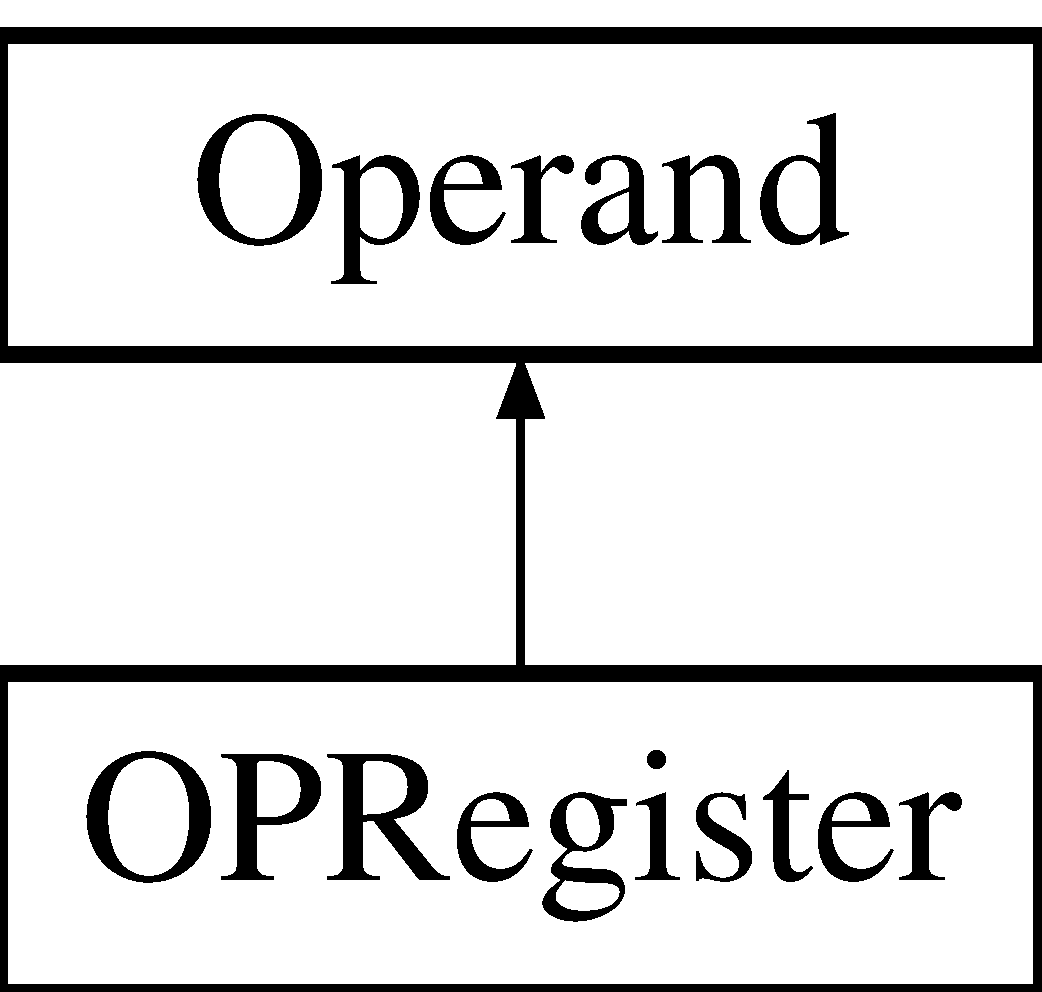
\includegraphics[height=2.000000cm]{classOPRegister}
\end{center}
\end{figure}
\subsection*{\-Public \-Member \-Functions}
\begin{DoxyCompactItemize}
\item 
\hypertarget{classOPRegister_a896eb65f36bf615ccfa74541de23858f}{\hyperlink{classOPRegister_a896eb65f36bf615ccfa74541de23858f}{\-O\-P\-Register} (string, t\-\_\-\-Src\-\_\-\-Dst)}\label{classOPRegister_a896eb65f36bf615ccfa74541de23858f}

\begin{DoxyCompactList}\small\item\em \-Constructor of the \-Register class. \end{DoxyCompactList}\item 
\hypertarget{classOPRegister_ad75c23d1db7c149c20cbc8bb01c6df59}{\hyperlink{classOPRegister_ad75c23d1db7c149c20cbc8bb01c6df59}{\-O\-P\-Register} (string, int, t\-\_\-\-Src\-\_\-\-Dst)}\label{classOPRegister_ad75c23d1db7c149c20cbc8bb01c6df59}

\begin{DoxyCompactList}\small\item\em \-Constructor of the \-Register class. \end{DoxyCompactList}\item 
\hypertarget{classOPRegister_a3c9786680764ada47370d469790b8178}{{\bfseries \-O\-P\-Register} (int, t\-\_\-\-Src\-\_\-\-Dst)}\label{classOPRegister_a3c9786680764ada47370d469790b8178}

\item 
\hypertarget{classOPRegister_aedab3bc5a2eecd0d02771fb6b37d73fe}{virtual \hyperlink{classOPRegister_aedab3bc5a2eecd0d02771fb6b37d73fe}{$\sim$\-O\-P\-Register} ()}\label{classOPRegister_aedab3bc5a2eecd0d02771fb6b37d73fe}

\begin{DoxyCompactList}\small\item\em \-Destructor of the \-Register class. \end{DoxyCompactList}\item 
int \hyperlink{classOPRegister_a2e42d6407677a7be154a5d4d74f7a8e7}{get\-\_\-reg} ()
\begin{DoxyCompactList}\small\item\em \-Get the \-Register value. \end{DoxyCompactList}\item 
\hypertarget{classOPRegister_ab514f45a9957e9b485fee38f264a70cf}{void \hyperlink{classOPRegister_ab514f45a9957e9b485fee38f264a70cf}{set\-\_\-reg} (int)}\label{classOPRegister_ab514f45a9957e9b485fee38f264a70cf}

\begin{DoxyCompactList}\small\item\em set the \-Register value setter of the \-Register \end{DoxyCompactList}\item 
virtual string \hyperlink{classOPRegister_a3f9f6cad40b83eee3f88a2e84a0ccffa}{get\-\_\-op} ()
\begin{DoxyCompactList}\small\item\em \-Get the operand value. \end{DoxyCompactList}\item 
virtual t\-\_\-\-Op\-Type \hyperlink{classOPRegister_a1be03d6e6422510a1fd12d1f13dfd601}{get\-\_\-op\-\_\-type} ()
\begin{DoxyCompactList}\small\item\em get the operator type \end{DoxyCompactList}\item 
virtual string \hyperlink{classOPRegister_a9f55bdff75224fb18973a9e913a4022f}{to\-\_\-string} ()
\begin{DoxyCompactList}\small\item\em tostring \end{DoxyCompactList}\item 
\hypertarget{classOPRegister_a3cceb6c804e4fe1187de7eb47c21a285}{virtual void \hyperlink{classOPRegister_a3cceb6c804e4fe1187de7eb47c21a285}{set\-\_\-op} (string)}\label{classOPRegister_a3cceb6c804e4fe1187de7eb47c21a285}

\begin{DoxyCompactList}\small\item\em set the operand value setter of the operand \end{DoxyCompactList}\item 
\hypertarget{classOPRegister_a23b5061c12e99d3bd320038e643eb247}{void \hyperlink{classOPRegister_a23b5061c12e99d3bd320038e643eb247}{set\-\_\-type} (t\-\_\-\-Src\-\_\-\-Dst)}\label{classOPRegister_a23b5061c12e99d3bd320038e643eb247}

\begin{DoxyCompactList}\small\item\em set the type of the register setter of the register type \end{DoxyCompactList}\item 
\hypertarget{classOPRegister_a7748867306b20ca99c0955b376789777}{t\-\_\-\-Src\-\_\-\-Dst \hyperlink{classOPRegister_a7748867306b20ca99c0955b376789777}{get\-\_\-type} ()}\label{classOPRegister_a7748867306b20ca99c0955b376789777}

\begin{DoxyCompactList}\small\item\em get the type of the register getter of the register type \end{DoxyCompactList}\end{DoxyCompactItemize}


\subsection{\-Detailed \-Description}
class representing a \-Register herited by \hyperlink{classOperand}{\-Operand} 

\subsection{\-Member \-Function \-Documentation}
\hypertarget{classOPRegister_a3f9f6cad40b83eee3f88a2e84a0ccffa}{\index{\-O\-P\-Register@{\-O\-P\-Register}!get\-\_\-op@{get\-\_\-op}}
\index{get\-\_\-op@{get\-\_\-op}!OPRegister@{\-O\-P\-Register}}
\subsubsection[{get\-\_\-op}]{\setlength{\rightskip}{0pt plus 5cm}virtual string {\bf \-O\-P\-Register\-::get\-\_\-op} (
\begin{DoxyParamCaption}
{}
\end{DoxyParamCaption}
)\hspace{0.3cm}{\ttfamily  \mbox{[}virtual\mbox{]}}}}\label{classOPRegister_a3f9f6cad40b83eee3f88a2e84a0ccffa}


\-Get the operand value. 

\begin{DoxyReturn}{\-Returns}
return the string of the register 
\end{DoxyReturn}


\-Implements \hyperlink{classOperand_a2bf3ad8b34d39cb35ff743ffcc0f4675}{\-Operand}.

\hypertarget{classOPRegister_a1be03d6e6422510a1fd12d1f13dfd601}{\index{\-O\-P\-Register@{\-O\-P\-Register}!get\-\_\-op\-\_\-type@{get\-\_\-op\-\_\-type}}
\index{get\-\_\-op\-\_\-type@{get\-\_\-op\-\_\-type}!OPRegister@{\-O\-P\-Register}}
\subsubsection[{get\-\_\-op\-\_\-type}]{\setlength{\rightskip}{0pt plus 5cm}virtual t\-\_\-\-Op\-Type {\bf \-O\-P\-Register\-::get\-\_\-op\-\_\-type} (
\begin{DoxyParamCaption}
{}
\end{DoxyParamCaption}
)\hspace{0.3cm}{\ttfamily  \mbox{[}virtual\mbox{]}}}}\label{classOPRegister_a1be03d6e6422510a1fd12d1f13dfd601}


get the operator type 

\begin{DoxyReturn}{\-Returns}
return the \hyperlink{classOperand}{\-Operand} type as enum 
\end{DoxyReturn}


\-Implements \hyperlink{classOperand_afd469e305a467e2574f34ac9bd6c62b0}{\-Operand}.

\hypertarget{classOPRegister_a2e42d6407677a7be154a5d4d74f7a8e7}{\index{\-O\-P\-Register@{\-O\-P\-Register}!get\-\_\-reg@{get\-\_\-reg}}
\index{get\-\_\-reg@{get\-\_\-reg}!OPRegister@{\-O\-P\-Register}}
\subsubsection[{get\-\_\-reg}]{\setlength{\rightskip}{0pt plus 5cm}int {\bf \-O\-P\-Register\-::get\-\_\-reg} (
\begin{DoxyParamCaption}
{}
\end{DoxyParamCaption}
)}}\label{classOPRegister_a2e42d6407677a7be154a5d4d74f7a8e7}


\-Get the \-Register value. 

\begin{DoxyReturn}{\-Returns}
return the number of the \-Register 
\end{DoxyReturn}
\hypertarget{classOPRegister_a9f55bdff75224fb18973a9e913a4022f}{\index{\-O\-P\-Register@{\-O\-P\-Register}!to\-\_\-string@{to\-\_\-string}}
\index{to\-\_\-string@{to\-\_\-string}!OPRegister@{\-O\-P\-Register}}
\subsubsection[{to\-\_\-string}]{\setlength{\rightskip}{0pt plus 5cm}virtual string {\bf \-O\-P\-Register\-::to\-\_\-string} (
\begin{DoxyParamCaption}
{}
\end{DoxyParamCaption}
)\hspace{0.3cm}{\ttfamily  \mbox{[}virtual\mbox{]}}}}\label{classOPRegister_a9f55bdff75224fb18973a9e913a4022f}


tostring 

\begin{DoxyReturn}{\-Returns}
return the \-Object as string 
\end{DoxyReturn}


\-Implements \hyperlink{classOperand_a28aed96d5fafee66be81c30c1435ad00}{\-Operand}.



\-The documentation for this class was generated from the following file\-:\begin{DoxyCompactItemize}
\item 
\hyperlink{OPRegister_8h}{\-O\-P\-Register.\-h}\end{DoxyCompactItemize}

\hypertarget{classProgram}{\section{\-Program \-Class \-Reference}
\label{classProgram}\index{\-Program@{\-Program}}
}


class representing a program as list of lines  




{\ttfamily \#include $<$\-Program.\-h$>$}

\subsection*{\-Public \-Member \-Functions}
\begin{DoxyCompactItemize}
\item 
\hypertarget{classProgram_aaefaa0df08f3484476fc4d61e97acbdc}{\hyperlink{classProgram_aaefaa0df08f3484476fc4d61e97acbdc}{\-Program} ()}\label{classProgram_aaefaa0df08f3484476fc4d61e97acbdc}

\begin{DoxyCompactList}\small\item\em \-Empty constructor of a program. \end{DoxyCompactList}\item 
\hypertarget{classProgram_a9918fe797bf830c47a652c81f449c35c}{\hyperlink{classProgram_a9918fe797bf830c47a652c81f449c35c}{\-Program} (\hyperlink{classProgram}{\-Program} const \&otherprogram)}\label{classProgram_a9918fe797bf830c47a652c81f449c35c}

\begin{DoxyCompactList}\small\item\em \-Copy constructor of a program. \end{DoxyCompactList}\item 
\hypertarget{classProgram_aabe3dfc72075de14b189b22b0e33ff23}{\hyperlink{classProgram_aabe3dfc72075de14b189b22b0e33ff23}{\-Program} (string const file)}\label{classProgram_aabe3dfc72075de14b189b22b0e33ff23}

\begin{DoxyCompactList}\small\item\em \-Constructor with the input file of program. \end{DoxyCompactList}\item 
\hypertarget{classProgram_a986aef1c50e1d338a3315a47ba6df549}{\hyperlink{classProgram_a986aef1c50e1d338a3315a47ba6df549}{$\sim$\-Program} ()}\label{classProgram_a986aef1c50e1d338a3315a47ba6df549}

\begin{DoxyCompactList}\small\item\em \-Destructor of program. \end{DoxyCompactList}\item 
\hypertarget{classProgram_a90e1c506dffd5756133f70811f6117d9}{void \hyperlink{classProgram_a90e1c506dffd5756133f70811f6117d9}{add\-\_\-line} (\hyperlink{classLine}{\-Line} $\ast$newline)}\label{classProgram_a90e1c506dffd5756133f70811f6117d9}

\begin{DoxyCompactList}\small\item\em \-Add a line at the end of the program. \end{DoxyCompactList}\item 
\hypertarget{classProgram_a7adb0709f1a9f3ed63e861cc7f02d308}{int \hyperlink{classProgram_a7adb0709f1a9f3ed63e861cc7f02d308}{add\-\_\-line\-\_\-at} (\hyperlink{classLine}{\-Line} $\ast$newline, int position)}\label{classProgram_a7adb0709f1a9f3ed63e861cc7f02d308}

\begin{DoxyCompactList}\small\item\em \-Add a line to the program with position as index. \end{DoxyCompactList}\item 
\hypertarget{classProgram_aabea8add836e10a384b63e2f293ece23}{void \hyperlink{classProgram_aabea8add836e10a384b63e2f293ece23}{exchange\-\_\-line} (int line1, int line2)}\label{classProgram_aabea8add836e10a384b63e2f293ece23}

\begin{DoxyCompactList}\small\item\em \-Reverse two lines which are at the index line1 and line2. \end{DoxyCompactList}\item 
\hypertarget{classProgram_a3c1399ac5ed69e5c152f1a2cc1e644d4}{void \hyperlink{classProgram_a3c1399ac5ed69e5c152f1a2cc1e644d4}{display} ()}\label{classProgram_a3c1399ac5ed69e5c152f1a2cc1e644d4}

\begin{DoxyCompactList}\small\item\em display the program \end{DoxyCompactList}\item 
\hypertarget{classProgram_a1adce5c1fc414a378e4b87f1d4b535e1}{void \hyperlink{classProgram_a1adce5c1fc414a378e4b87f1d4b535e1}{del\-\_\-line} (int index)}\label{classProgram_a1adce5c1fc414a378e4b87f1d4b535e1}

\begin{DoxyCompactList}\small\item\em \-Delete the line at the given index in the program. \end{DoxyCompactList}\item 
\hypertarget{classProgram_ae897b48e1e1be99578440eb6a38a3a0d}{\hyperlink{classLine}{\-Line} $\ast$ \hyperlink{classProgram_ae897b48e1e1be99578440eb6a38a3a0d}{find\-\_\-line} (int index)}\label{classProgram_ae897b48e1e1be99578440eb6a38a3a0d}

\begin{DoxyCompactList}\small\item\em gives the line that corresponds to the index \end{DoxyCompactList}\item 
\hypertarget{classProgram_a190f24ecadca14d748408c352aabc219}{int \hyperlink{classProgram_a190f24ecadca14d748408c352aabc219}{size} ()}\label{classProgram_a190f24ecadca14d748408c352aabc219}

\begin{DoxyCompactList}\small\item\em get the length of the program \end{DoxyCompactList}\item 
void \hyperlink{classProgram_a3db3e17c96bb809c3e6f81b8bc22ee20}{in\-\_\-file} (string const filename)
\begin{DoxyCompactList}\small\item\em returns the dependance betwen the two given instructions \end{DoxyCompactList}\item 
\hypertarget{classProgram_aff32c461ae544453df5d55f475b3da22}{bool \hyperlink{classProgram_aff32c461ae544453df5d55f475b3da22}{is\-\_\-empty} ()}\label{classProgram_aff32c461ae544453df5d55f475b3da22}

\begin{DoxyCompactList}\small\item\em return true if the program is \-Empty \end{DoxyCompactList}\item 
\hypertarget{classProgram_aa2111257b1f690520316e4831e55798d}{void \hyperlink{classProgram_aa2111257b1f690520316e4831e55798d}{comput\-\_\-function} ()}\label{classProgram_aa2111257b1f690520316e4831e55798d}

\begin{DoxyCompactList}\small\item\em calculate the functions of the program \end{DoxyCompactList}\item 
\hypertarget{classProgram_aa85073d3bd6782af3759f4a2961ae80f}{int \hyperlink{classProgram_aa85073d3bd6782af3759f4a2961ae80f}{nbr\-\_\-func} ()}\label{classProgram_aa85073d3bd6782af3759f4a2961ae80f}

\begin{DoxyCompactList}\small\item\em get the number of functions in the program \end{DoxyCompactList}\item 
\hypertarget{classProgram_aea6d5c7367bbee48ec5cbb295ef6fd5f}{\hyperlink{classFunction}{\-Function} $\ast$ \hyperlink{classProgram_aea6d5c7367bbee48ec5cbb295ef6fd5f}{get\-\_\-function} (int index)}\label{classProgram_aea6d5c7367bbee48ec5cbb295ef6fd5f}

\begin{DoxyCompactList}\small\item\em returns the function of index index in the list \-\_\-myfunc \end{DoxyCompactList}\item 
\hypertarget{classProgram_a88b4499bd1a7485d7492fc812b957899}{list$<$ \hyperlink{classFunction}{\-Function} $\ast$ $>$\-::iterator {\bfseries function\-\_\-list\-\_\-begin} ()}\label{classProgram_a88b4499bd1a7485d7492fc812b957899}

\item 
\hypertarget{classProgram_a7507c914934f6847c6a4e19dae13cdf3}{list$<$ \hyperlink{classFunction}{\-Function} $\ast$ $>$\-::iterator {\bfseries function\-\_\-list\-\_\-end} ()}\label{classProgram_a7507c914934f6847c6a4e19dae13cdf3}

\item 
\hypertarget{classProgram_a1cef65227311c68a2e81c89dcbc16914}{void \hyperlink{classProgram_a1cef65227311c68a2e81c89dcbc16914}{flush} ()}\label{classProgram_a1cef65227311c68a2e81c89dcbc16914}

\begin{DoxyCompactList}\small\item\em empty the program \end{DoxyCompactList}\item 
\hypertarget{classProgram_a0d1d9386925418b5fd0a09bf5de16208}{void \hyperlink{classProgram_a0d1d9386925418b5fd0a09bf5de16208}{comput\-\_\-\-C\-F\-G} ()}\label{classProgram_a0d1d9386925418b5fd0a09bf5de16208}

\begin{DoxyCompactList}\small\item\em calculate the \-C\-F\-G associated with each function of the program \end{DoxyCompactList}\item 
\hypertarget{classProgram_a69ddee195c76bff05733d927e315f319}{\hyperlink{classCfg}{\-Cfg} $\ast$ \hyperlink{classProgram_a69ddee195c76bff05733d927e315f319}{get\-\_\-\-C\-F\-G} (int index)}\label{classProgram_a69ddee195c76bff05733d927e315f319}

\begin{DoxyCompactList}\small\item\em returns the \-C\-F\-G of index index in the list \-\_\-my\-C\-F\-G \end{DoxyCompactList}\end{DoxyCompactItemize}


\subsection{\-Detailed \-Description}
class representing a program as list of lines 

\subsection{\-Member \-Function \-Documentation}
\hypertarget{classProgram_a3db3e17c96bb809c3e6f81b8bc22ee20}{\index{\-Program@{\-Program}!in\-\_\-file@{in\-\_\-file}}
\index{in\-\_\-file@{in\-\_\-file}!Program@{\-Program}}
\subsubsection[{in\-\_\-file}]{\setlength{\rightskip}{0pt plus 5cm}void {\bf \-Program\-::in\-\_\-file} (
\begin{DoxyParamCaption}
\item[{string const}]{filename}
\end{DoxyParamCaption}
)}}\label{classProgram_a3db3e17c96bb809c3e6f81b8bc22ee20}


returns the dependance betwen the two given instructions 

\begin{DoxyReturn}{\-Returns}
returns the dependance in the enum formatwrite the programme into a file 
\end{DoxyReturn}


\-The documentation for this class was generated from the following file\-:\begin{DoxyCompactItemize}
\item 
\hyperlink{Program_8h}{\-Program.\-h}\end{DoxyCompactItemize}

\hypertarget{structs__Profile}{\section{s\-\_\-\-Profile \-Struct \-Reference}
\label{structs__Profile}\index{s\-\_\-\-Profile@{s\-\_\-\-Profile}}
}


\-Structure allowing to add caracteristics to an operator.  




{\ttfamily \#include $<$\-Enum\-\_\-type.\-h$>$}

\subsection*{\-Public \-Attributes}
\begin{DoxyCompactItemize}
\item 
\hypertarget{structs__Profile_a3debabafa904b8f4c5e7bf2bda2a5e60}{t\-\_\-\-Operator {\bfseries op}}\label{structs__Profile_a3debabafa904b8f4c5e7bf2bda2a5e60}

\item 
\hypertarget{structs__Profile_ab9f52013690834dd36766d356c90c449}{std\-::string {\bfseries nom}}\label{structs__Profile_ab9f52013690834dd36766d356c90c449}

\item 
\hypertarget{structs__Profile_ae8153795530389f76f6c56bdeac40d46}{t\-\_\-\-Format {\bfseries format}}\label{structs__Profile_ae8153795530389f76f6c56bdeac40d46}

\item 
\hypertarget{structs__Profile_a2a8c53bcb4fb28c3aa368a27954d9b1b}{t\-\_\-\-Inst {\bfseries type}}\label{structs__Profile_a2a8c53bcb4fb28c3aa368a27954d9b1b}

\item 
\hypertarget{structs__Profile_a7930c41fdfa4249a1c147edf7ac68822}{int {\bfseries nb\-\_\-oper}}\label{structs__Profile_a7930c41fdfa4249a1c147edf7ac68822}

\end{DoxyCompactItemize}


\subsection{\-Detailed \-Description}
\-Structure allowing to add caracteristics to an operator. 

\-The documentation for this struct was generated from the following file\-:\begin{DoxyCompactItemize}
\item 
\-Enum\-\_\-type.\-h\end{DoxyCompactItemize}

\hypertarget{classTestOPLabel}{\section{\-Test\-O\-P\-Label \-Class \-Reference}
\label{classTestOPLabel}\index{\-Test\-O\-P\-Label@{\-Test\-O\-P\-Label}}
}
\subsection*{\-Public \-Member \-Functions}
\begin{DoxyCompactItemize}
\item 
\hypertarget{classTestOPLabel_a9ddb0e7ab19700d5bf73490ba0ebbf36}{void {\bfseries set\-Up} (void)}\label{classTestOPLabel_a9ddb0e7ab19700d5bf73490ba0ebbf36}

\item 
\hypertarget{classTestOPLabel_a6bc3fb561309973920fe3abc020facf1}{void {\bfseries tear\-Down} (void)}\label{classTestOPLabel_a6bc3fb561309973920fe3abc020facf1}

\end{DoxyCompactItemize}


\-The documentation for this class was generated from the following file\-:\begin{DoxyCompactItemize}
\item 
\-Test\-O\-P\-Label.\-h\end{DoxyCompactItemize}

\hypertarget{structutchn}{\section{utchn \-Struct \-Reference}
\label{structutchn}\index{utchn@{utchn}}
}
\subsection*{\-Public \-Attributes}
\begin{DoxyCompactItemize}
\item 
\hypertarget{structutchn_adf89384022b2de9cb3a0be987e746bbe}{struct \hyperlink{structutchn}{utchn} $\ast$ {\bfseries \-N\-E\-X\-T}}\label{structutchn_adf89384022b2de9cb3a0be987e746bbe}

\item 
\hypertarget{structutchn_a4c8453ea9877abcfdb65a88f3497a294}{union \hyperlink{unionutdat}{utdat} {\bfseries \-D\-A\-T\-A}}\label{structutchn_a4c8453ea9877abcfdb65a88f3497a294}

\end{DoxyCompactItemize}


\-The documentation for this struct was generated from the following file\-:\begin{DoxyCompactItemize}
\item 
utl200.\-h\end{DoxyCompactItemize}

\hypertarget{unionutdat}{\section{utdat \-Union \-Reference}
\label{unionutdat}\index{utdat@{utdat}}
}
\subsection*{\-Public \-Attributes}
\begin{DoxyCompactItemize}
\item 
\hypertarget{unionutdat_a3f76aa32eacd8c9a18af99d01be467c2}{void $\ast$ {\bfseries \-V\-P\-N\-T}}\label{unionutdat_a3f76aa32eacd8c9a18af99d01be467c2}

\item 
\hypertarget{unionutdat_ae0e7486135096802136dc1cd41c9a005}{float {\bfseries \-F\-L\-O\-T}}\label{unionutdat_ae0e7486135096802136dc1cd41c9a005}

\item 
\hypertarget{unionutdat_aae5fc4b76253540a8c4e983e162072be}{unsigned int {\bfseries \-U\-I\-N\-T}}\label{unionutdat_aae5fc4b76253540a8c4e983e162072be}

\item 
\hypertarget{unionutdat_a5bf144421cb7bf3264438be37aa5d884}{int {\bfseries \-S\-I\-N\-T}}\label{unionutdat_a5bf144421cb7bf3264438be37aa5d884}

\item 
\hypertarget{unionutdat_afad7210b163e44fc45ba5d19f9354b73}{char {\bfseries \-C\-H\-A\-R}}\label{unionutdat_afad7210b163e44fc45ba5d19f9354b73}

\item 
\hypertarget{unionutdat_ac716e252c27e7f050371d9c28b4c75f4}{unsigned char {\bfseries \-U\-C\-H\-R}}\label{unionutdat_ac716e252c27e7f050371d9c28b4c75f4}

\end{DoxyCompactItemize}


\-The documentation for this union was generated from the following file\-:\begin{DoxyCompactItemize}
\item 
utl200.\-h\end{DoxyCompactItemize}

\hypertarget{structutdic}{\section{utdic Struct Reference}
\label{structutdic}\index{utdic@{utdic}}
}
\subsection*{Public Attributes}
\begin{DoxyCompactItemize}
\item 
\hypertarget{structutdic_afa286d4adfb2ac8a02c022cc635057b0}{struct \hyperlink{structutdic}{utdic} $\ast$ {\bfseries N\-E\-X\-T}}\label{structutdic_afa286d4adfb2ac8a02c022cc635057b0}

\item 
\hypertarget{structutdic_a04eed0ebafe9ecb10bf6126f332f4969}{struct \hyperlink{structutdit}{utdit} $\ast$ {\bfseries T\-A\-B\-L\-E}}\label{structutdic_a04eed0ebafe9ecb10bf6126f332f4969}

\item 
\hypertarget{structutdic_a471d6eb0acb36915182e380eb4ab15da}{void $\ast$($\ast$ {\bfseries A\-D\-D\-\_\-\-K} )()}\label{structutdic_a471d6eb0acb36915182e380eb4ab15da}

\item 
\hypertarget{structutdic_ade72458bf8aae6928960a0b66e1fce45}{void($\ast$ {\bfseries F\-R\-E\-\_\-\-K} )()}\label{structutdic_ade72458bf8aae6928960a0b66e1fce45}

\item 
\hypertarget{structutdic_a5bd02f97e36b6e5d5742339a3eb65774}{int($\ast$ {\bfseries C\-M\-P\-\_\-\-K} )()}\label{structutdic_a5bd02f97e36b6e5d5742339a3eb65774}

\item 
\hypertarget{structutdic_a790b0db53ecc9b661184ce9407ab07e1}{void $\ast$($\ast$ {\bfseries A\-D\-D\-\_\-\-D} )()}\label{structutdic_a790b0db53ecc9b661184ce9407ab07e1}

\item 
\hypertarget{structutdic_a7a15dea48310ad7a9cf99bbc8d92373a}{void($\ast$ {\bfseries F\-R\-E\-\_\-\-D} )()}\label{structutdic_a7a15dea48310ad7a9cf99bbc8d92373a}

\item 
\hypertarget{structutdic_a55b256d7dd0c56b55811b9b8ace8796b}{unsigned int($\ast$ {\bfseries H\-S\-H\-\_\-\-K} )()}\label{structutdic_a55b256d7dd0c56b55811b9b8ace8796b}

\item 
\hypertarget{structutdic_a55eabe5e987e0fbe7683b3c938390e56}{unsigned short {\bfseries S\-I\-Z\-E}}\label{structutdic_a55eabe5e987e0fbe7683b3c938390e56}

\item 
\hypertarget{structutdic_a797453db20732c62ffb3603de50d88a9}{unsigned short {\bfseries S\-P\-E\-E\-D}}\label{structutdic_a797453db20732c62ffb3603de50d88a9}

\item 
\hypertarget{structutdic_a5ac9d099e722a47666b07c10f155b503}{unsigned int {\bfseries I\-N\-I\-T}}\label{structutdic_a5ac9d099e722a47666b07c10f155b503}

\item 
\hypertarget{structutdic_a66864a2a75e70334df90b8fb4dff592f}{unsigned int {\bfseries S\-T\-A\-T\-U\-S}}\label{structutdic_a66864a2a75e70334df90b8fb4dff592f}

\item 
\hypertarget{structutdic_a1cc5230f2a4edd235bbcb11ba492c5a9}{unsigned int {\bfseries F\-L\-A\-G}}\label{structutdic_a1cc5230f2a4edd235bbcb11ba492c5a9}

\end{DoxyCompactItemize}


The documentation for this struct was generated from the following file\-:\begin{DoxyCompactItemize}
\item 
utl200.\-h\end{DoxyCompactItemize}

\hypertarget{structutdit}{\section{utdit Struct Reference}
\label{structutdit}\index{utdit@{utdit}}
}
\subsection*{Public Attributes}
\begin{DoxyCompactItemize}
\item 
\hypertarget{structutdit_a35be07ef8c6bf95874e1569b1c2a446a}{struct \hyperlink{structuttyp}{uttyp} $\ast$ {\bfseries I\-T\-E\-M}}\label{structutdit_a35be07ef8c6bf95874e1569b1c2a446a}

\end{DoxyCompactItemize}


The documentation for this struct was generated from the following file\-:\begin{DoxyCompactItemize}
\item 
utl200.\-h\end{DoxyCompactItemize}

\hypertarget{structuttdc}{\section{uttdc \-Struct \-Reference}
\label{structuttdc}\index{uttdc@{uttdc}}
}
\subsection*{\-Public \-Attributes}
\begin{DoxyCompactItemize}
\item 
\hypertarget{structuttdc_a36ecbdb0a7090fabe5bfdafe71d29e1c}{struct \hyperlink{structuttdc}{uttdc} $\ast$ {\bfseries \-N\-E\-X\-T}}\label{structuttdc_a36ecbdb0a7090fabe5bfdafe71d29e1c}

\item 
\hypertarget{structuttdc_ad03c46371086203aa425921abb0e39ef}{union \hyperlink{unionutdat}{utdat} {\bfseries \-D\-A\-T1}}\label{structuttdc_ad03c46371086203aa425921abb0e39ef}

\item 
\hypertarget{structuttdc_adce9c114f323143827917a9ba99db1b4}{union \hyperlink{unionutdat}{utdat} {\bfseries \-D\-A\-T2}}\label{structuttdc_adce9c114f323143827917a9ba99db1b4}

\item 
\hypertarget{structuttdc_ae45fd296fefee3b446fa004fae80b737}{union \hyperlink{unionutdat}{utdat} {\bfseries \-D\-A\-T3}}\label{structuttdc_ae45fd296fefee3b446fa004fae80b737}

\end{DoxyCompactItemize}


\-The documentation for this struct was generated from the following file\-:\begin{DoxyCompactItemize}
\item 
utl200.\-h\end{DoxyCompactItemize}

\hypertarget{structuttpd}{\section{uttpd Struct Reference}
\label{structuttpd}\index{uttpd@{uttpd}}
}
\subsection*{Public Attributes}
\begin{DoxyCompactItemize}
\item 
\hypertarget{structuttpd_a5cb5f6e1386d4d1a421db63a9f296879}{struct \hyperlink{structuttpd}{uttpd} $\ast$ {\bfseries N\-E\-X\-T}}\label{structuttpd_a5cb5f6e1386d4d1a421db63a9f296879}

\item 
\hypertarget{structuttpd_a5dc0039ca809f7aa4f582b830c005762}{union \hyperlink{unionutdat}{utdat} {\bfseries D\-A\-T1}}\label{structuttpd_a5dc0039ca809f7aa4f582b830c005762}

\item 
\hypertarget{structuttpd_adaea4e4a8db887e61b8944d75c5be2a3}{double {\bfseries D\-A\-T2}}\label{structuttpd_adaea4e4a8db887e61b8944d75c5be2a3}

\end{DoxyCompactItemize}


The documentation for this struct was generated from the following file\-:\begin{DoxyCompactItemize}
\item 
utl200.\-h\end{DoxyCompactItemize}

\hypertarget{structuttyp}{\section{uttyp Struct Reference}
\label{structuttyp}\index{uttyp@{uttyp}}
}
\subsection*{Public Attributes}
\begin{DoxyCompactItemize}
\item 
\hypertarget{structuttyp_aeb2e67b550626f318c8627127cac0f10}{struct \hyperlink{structuttyp}{uttyp} $\ast$ {\bfseries N\-E\-X\-T}}\label{structuttyp_aeb2e67b550626f318c8627127cac0f10}

\item 
\hypertarget{structuttyp_a8c93cab3549706951c3785e1aec42242}{union \hyperlink{unionutdat}{utdat} {\bfseries D\-A\-T1}}\label{structuttyp_a8c93cab3549706951c3785e1aec42242}

\item 
\hypertarget{structuttyp_a8d2dd6929a5e74e498543bf759ba1bea}{union \hyperlink{unionutdat}{utdat} {\bfseries D\-A\-T2}}\label{structuttyp_a8d2dd6929a5e74e498543bf759ba1bea}

\end{DoxyCompactItemize}


The documentation for this struct was generated from the following file\-:\begin{DoxyCompactItemize}
\item 
utl200.\-h\end{DoxyCompactItemize}

\hypertarget{unionYYSTYPE}{\section{\-Y\-Y\-S\-T\-Y\-P\-E \-Union \-Reference}
\label{unionYYSTYPE}\index{\-Y\-Y\-S\-T\-Y\-P\-E@{\-Y\-Y\-S\-T\-Y\-P\-E}}
}
\subsection*{\-Public \-Attributes}
\begin{DoxyCompactItemize}
\item 
\hypertarget{unionYYSTYPE_a4b9cb65f9c58be454aa7c4b25698d709}{struct \hyperlink{structutchn}{utchn} $\ast$ {\bfseries pchn}}\label{unionYYSTYPE_a4b9cb65f9c58be454aa7c4b25698d709}

\item 
\hypertarget{unionYYSTYPE_a8ea73faccde5303458c8eae598a8bef4}{unsigned int {\bfseries uval}}\label{unionYYSTYPE_a8ea73faccde5303458c8eae598a8bef4}

\item 
\hypertarget{unionYYSTYPE_a9208e91d3ca5483b43d8c1fbd7be4ce6}{char $\ast$ {\bfseries text}}\label{unionYYSTYPE_a9208e91d3ca5483b43d8c1fbd7be4ce6}

\end{DoxyCompactItemize}


\-The documentation for this union was generated from the following file\-:\begin{DoxyCompactItemize}
\item 
asm\-\_\-mipsyac.\-h\end{DoxyCompactItemize}

\chapter{\-File \-Documentation}
\hypertarget{Basic__block_8h}{\section{\-Basic\-\_\-block.\-h \-File \-Reference}
\label{Basic__block_8h}\index{\-Basic\-\_\-block.\-h@{\-Basic\-\_\-block.\-h}}
}


\hyperlink{classBasic__block}{\-Basic\-\_\-block} class.  


{\ttfamily \#include $<$\-Node.\-h$>$}\*
{\ttfamily \#include $<$\-Instruction.\-h$>$}\*
{\ttfamily \#include $<$string$>$}\*
{\ttfamily \#include $<$stdio.\-h$>$}\*
{\ttfamily \#include $<$\-Enum\-\_\-type.\-h$>$}\*
{\ttfamily \#include $<$fstream$>$}\*
{\ttfamily \#include $<$list$>$}\*
{\ttfamily \#include $<$\-Dfg.\-h$>$}\*
{\ttfamily \#include $<$\-Node\-\_\-dfg.\-h$>$}\*
\subsection*{\-Classes}
\begin{DoxyCompactItemize}
\item 
class \hyperlink{classBasic__block}{\-Basic\-\_\-block}
\begin{DoxyCompactList}\small\item\em class representing a \hyperlink{classBasic__block}{\-Basic\-\_\-block} of a fonction \end{DoxyCompactList}\item 
struct {\bfseries \-Basic\-\_\-block\-::def\-\_\-use\-\_\-t}
\end{DoxyCompactItemize}
\subsection*{\-Defines}
\begin{DoxyCompactItemize}
\item 
\hypertarget{Basic__block_8h_a8504d47471a8b24cbba3cd57c1cb7844}{\#define {\bfseries \-N\-B\-\_\-\-R\-E\-G\-I\-S\-T\-R\-E\-S}~32}\label{Basic__block_8h_a8504d47471a8b24cbba3cd57c1cb7844}

\end{DoxyCompactItemize}


\subsection{\-Detailed \-Description}
\hyperlink{classBasic__block}{\-Basic\-\_\-block} class. \begin{DoxyAuthor}{\-Author}
\-Hajjem 
\end{DoxyAuthor}

\hypertarget{Cfg_8h}{\section{\-Cfg.\-h \-File \-Reference}
\label{Cfg_8h}\index{\-Cfg.\-h@{\-Cfg.\-h}}
}


\hyperlink{classCfg}{\-Cfg} class.  


{\ttfamily \#include $<$\-Basic\-\_\-block.\-h$>$}\*
{\ttfamily \#include $<$string$>$}\*
{\ttfamily \#include $<$stdio.\-h$>$}\*
{\ttfamily \#include $<$\-Label.\-h$>$}\*
{\ttfamily \#include $<$\-Enum\-\_\-type.\-h$>$}\*
{\ttfamily \#include $<$list$>$}\*
{\ttfamily \#include $<$fstream$>$}\*
\subsection*{\-Classes}
\begin{DoxyCompactItemize}
\item 
class \hyperlink{classCfg}{\-Cfg}
\begin{DoxyCompactList}\small\item\em class representing control flow graph \end{DoxyCompactList}\end{DoxyCompactItemize}


\subsection{\-Detailed \-Description}
\hyperlink{classCfg}{\-Cfg} class. \begin{DoxyAuthor}{\-Author}
\-Hajjem 
\end{DoxyAuthor}

\hypertarget{Dfg_8h}{\section{\-Dfg.\-h \-File \-Reference}
\label{Dfg_8h}\index{\-Dfg.\-h@{\-Dfg.\-h}}
}


\hyperlink{classDfg}{\-Dfg} class.  


{\ttfamily \#include $<$\-Node\-\_\-dfg.\-h$>$}\*
{\ttfamily \#include $<$\-Instruction.\-h$>$}\*
{\ttfamily \#include $<$\-Enum\-\_\-type.\-h$>$}\*
{\ttfamily \#include $<$fstream$>$}\*
{\ttfamily \#include $<$list$>$}\*
{\ttfamily \#include $<$boost/graph/adjacency\-\_\-list.\-hpp$>$}\*
{\ttfamily \#include $<$boost/graph/astar\-\_\-search.\-hpp$>$}\*
\subsection*{\-Classes}
\begin{DoxyCompactItemize}
\item 
class \hyperlink{classDfg}{\-Dfg}
\begin{DoxyCompactList}\small\item\em class representing a \hyperlink{classDfg}{\-Dfg} of a \-Basic block, a data flow graph that is to be used to calculate the critical path and schedule code \end{DoxyCompactList}\end{DoxyCompactItemize}


\subsection{\-Detailed \-Description}
\hyperlink{classDfg}{\-Dfg} class. \begin{DoxyAuthor}{\-Author}
\-Hajjem 
\end{DoxyAuthor}

\hypertarget{Directive_8h}{\section{\-Directive.\-h \-File \-Reference}
\label{Directive_8h}\index{\-Directive.\-h@{\-Directive.\-h}}
}


\hyperlink{classDirective}{\-Directive} class.  


{\ttfamily \#include $<$iostream$>$}\*
{\ttfamily \#include $<$string$>$}\*
{\ttfamily \#include $<$\-Enum\-\_\-type.\-h$>$}\*
{\ttfamily \#include $<$\-Line.\-h$>$}\*
\subsection*{\-Classes}
\begin{DoxyCompactItemize}
\item 
class \hyperlink{classDirective}{\-Directive}
\begin{DoxyCompactList}\small\item\em class representing an \hyperlink{classDirective}{\-Directive} herited by \hyperlink{classLine}{\-Line} \end{DoxyCompactList}\end{DoxyCompactItemize}


\subsection{\-Detailed \-Description}
\hyperlink{classDirective}{\-Directive} class. \begin{DoxyAuthor}{\-Author}
\-Hajjem 
\end{DoxyAuthor}

\hypertarget{Function_8h}{\section{\-Function.\-h \-File \-Reference}
\label{Function_8h}\index{\-Function.\-h@{\-Function.\-h}}
}


\hyperlink{classFunction}{\-Function} class.  


{\ttfamily \#include $<$\-Node.\-h$>$}\*
{\ttfamily \#include $<$\-Basic\-\_\-block.\-h$>$}\*
{\ttfamily \#include $<$\-Instruction.\-h$>$}\*
{\ttfamily \#include $<$string$>$}\*
{\ttfamily \#include $<$stdio.\-h$>$}\*
{\ttfamily \#include $<$\-Label.\-h$>$}\*
{\ttfamily \#include $<$\-Enum\-\_\-type.\-h$>$}\*
{\ttfamily \#include $<$list$>$}\*
{\ttfamily \#include $<$\-Cfg.\-h$>$}\*
{\ttfamily \#include $<$fstream$>$}\*
\subsection*{\-Classes}
\begin{DoxyCompactItemize}
\item 
class \hyperlink{classFunction}{\-Function}
\begin{DoxyCompactList}\small\item\em class representing a \hyperlink{classFunction}{\-Function} on a program \end{DoxyCompactList}\end{DoxyCompactItemize}


\subsection{\-Detailed \-Description}
\hyperlink{classFunction}{\-Function} class. \begin{DoxyAuthor}{\-Author}
\-Hajjem 
\end{DoxyAuthor}

\hypertarget{Instruction_8h}{\section{\-Instruction.\-h \-File \-Reference}
\label{Instruction_8h}\index{\-Instruction.\-h@{\-Instruction.\-h}}
}


\hyperlink{classInstruction}{\-Instruction} class.  


{\ttfamily \#include $<$\-Operand.\-h$>$}\*
{\ttfamily \#include $<$string$>$}\*
{\ttfamily \#include $<$\-O\-P\-Expression.\-h$>$}\*
{\ttfamily \#include $<$\-O\-P\-Immediate.\-h$>$}\*
{\ttfamily \#include $<$\-O\-P\-Label.\-h$>$}\*
{\ttfamily \#include $<$\-Line.\-h$>$}\*
{\ttfamily \#include $<$\-O\-P\-Register.\-h$>$}\*
{\ttfamily \#include $<$\-Enum\-\_\-type.\-h$>$}\*
{\ttfamily \#include $<$list$>$}\*
\subsection*{\-Classes}
\begin{DoxyCompactItemize}
\item 
struct \hyperlink{structdep}{dep}
\item 
class \hyperlink{classInstruction}{\-Instruction}
\begin{DoxyCompactList}\small\item\em class representing an instruction which herited by \hyperlink{classLine}{\-Line} \end{DoxyCompactList}\end{DoxyCompactItemize}


\subsection{\-Detailed \-Description}
\hyperlink{classInstruction}{\-Instruction} class. \begin{DoxyAuthor}{\-Author}
\-Hajjem -\/ \-Heydemann -\/ \-Girault 
\end{DoxyAuthor}

\hypertarget{Label_8h}{\section{\-Label.\-h \-File \-Reference}
\label{Label_8h}\index{\-Label.\-h@{\-Label.\-h}}
}


\hyperlink{classLabel}{\-Label} class.  


{\ttfamily \#include $<$iostream$>$}\*
{\ttfamily \#include $<$string$>$}\*
{\ttfamily \#include $<$\-Enum\-\_\-type.\-h$>$}\*
{\ttfamily \#include $<$\-Line.\-h$>$}\*
\subsection*{\-Classes}
\begin{DoxyCompactItemize}
\item 
class \hyperlink{classLabel}{\-Label}
\begin{DoxyCompactList}\small\item\em class representing an \hyperlink{classLabel}{\-Label} herited by \hyperlink{classLine}{\-Line} \end{DoxyCompactList}\end{DoxyCompactItemize}


\subsection{\-Detailed \-Description}
\hyperlink{classLabel}{\-Label} class. \begin{DoxyAuthor}{\-Author}
\-Hajjem 
\end{DoxyAuthor}

\hypertarget{Line_8h}{\section{\-Line.\-h \-File \-Reference}
\label{Line_8h}\index{\-Line.\-h@{\-Line.\-h}}
}


\hyperlink{classLine}{\-Line} class.  


{\ttfamily \#include $<$iostream$>$}\*
{\ttfamily \#include $<$string$>$}\*
{\ttfamily \#include $<$\-Enum\-\_\-type.\-h$>$}\*
\subsection*{\-Classes}
\begin{DoxyCompactItemize}
\item 
class \hyperlink{classLine}{\-Line}
\begin{DoxyCompactList}\small\item\em \-Abstract class representing an \hyperlink{classLine}{\-Line}. \end{DoxyCompactList}\end{DoxyCompactItemize}


\subsection{\-Detailed \-Description}
\hyperlink{classLine}{\-Line} class. \begin{DoxyAuthor}{\-Author}
\-Hajjem 
\end{DoxyAuthor}

\hypertarget{Node_8h}{\section{\-Node.\-h \-File \-Reference}
\label{Node_8h}\index{\-Node.\-h@{\-Node.\-h}}
}


\hyperlink{classNode}{\-Node} class.  


{\ttfamily \#include $<$\-Line.\-h$>$}\*
{\ttfamily \#include $<$string$>$}\*
{\ttfamily \#include $<$\-Enum\-\_\-type.\-h$>$}\*
\subsection*{\-Classes}
\begin{DoxyCompactItemize}
\item 
class \hyperlink{classNode}{\-Node}
\begin{DoxyCompactList}\small\item\em class representing a \hyperlink{classNode}{\-Node} in list \end{DoxyCompactList}\end{DoxyCompactItemize}


\subsection{\-Detailed \-Description}
\hyperlink{classNode}{\-Node} class. \begin{DoxyAuthor}{\-Author}
\-Hajjem 
\end{DoxyAuthor}

\hypertarget{Node__dfg_8h}{\section{\-Node\-\_\-dfg.\-h \-File \-Reference}
\label{Node__dfg_8h}\index{\-Node\-\_\-dfg.\-h@{\-Node\-\_\-dfg.\-h}}
}


\hyperlink{classNode__dfg}{\-Node\-\_\-dfg} class.  


{\ttfamily \#include $<$\-Basic\-\_\-block.\-h$>$}\*
{\ttfamily \#include $<$string$>$}\*
{\ttfamily \#include $<$stdio.\-h$>$}\*
{\ttfamily \#include $<$\-Label.\-h$>$}\*
{\ttfamily \#include $<$\-Enum\-\_\-type.\-h$>$}\*
\subsection*{\-Classes}
\begin{DoxyCompactItemize}
\item 
struct \hyperlink{structArc__t}{\-Arc\-\_\-t}
\item 
class \hyperlink{classNode__dfg}{\-Node\-\_\-dfg}
\begin{DoxyCompactList}\small\item\em class representing a node of data flow graph \end{DoxyCompactList}\end{DoxyCompactItemize}


\subsection{\-Detailed \-Description}
\hyperlink{classNode__dfg}{\-Node\-\_\-dfg} class. \begin{DoxyAuthor}{\-Author}
\-Hajjem 
\end{DoxyAuthor}

\hypertarget{Operand_8h}{\section{\-Operand.\-h \-File \-Reference}
\label{Operand_8h}\index{\-Operand.\-h@{\-Operand.\-h}}
}


\hyperlink{classOperand}{\-Operand} class.  


{\ttfamily \#include $<$iostream$>$}\*
{\ttfamily \#include $<$string$>$}\*
{\ttfamily \#include $<$\-Enum\-\_\-type.\-h$>$}\*
\subsection*{\-Classes}
\begin{DoxyCompactItemize}
\item 
class \hyperlink{classOperand}{\-Operand}
\begin{DoxyCompactList}\small\item\em \-Abstract class representing an operand. \end{DoxyCompactList}\end{DoxyCompactItemize}


\subsection{\-Detailed \-Description}
\hyperlink{classOperand}{\-Operand} class. \begin{DoxyAuthor}{\-Author}
\-Hajjem 
\end{DoxyAuthor}

\hypertarget{OPExpression_8h}{\section{\-O\-P\-Expression.\-h \-File \-Reference}
\label{OPExpression_8h}\index{\-O\-P\-Expression.\-h@{\-O\-P\-Expression.\-h}}
}


\hyperlink{classOPExpression}{\-O\-P\-Expression} class.  


{\ttfamily \#include $<$iostream$>$}\*
{\ttfamily \#include $<$string$>$}\*
{\ttfamily \#include $<$\-Operand.\-h$>$}\*
{\ttfamily \#include $<$\-Enum\-\_\-type.\-h$>$}\*
\subsection*{\-Classes}
\begin{DoxyCompactItemize}
\item 
class \hyperlink{classOPExpression}{\-O\-P\-Expression}
\begin{DoxyCompactList}\small\item\em class representing an expression herited by \hyperlink{classOperand}{\-Operand} \end{DoxyCompactList}\end{DoxyCompactItemize}


\subsection{\-Detailed \-Description}
\hyperlink{classOPExpression}{\-O\-P\-Expression} class. \begin{DoxyAuthor}{\-Author}
\-Hajjem 
\end{DoxyAuthor}

\hypertarget{OPImmediate_8h}{\section{\-O\-P\-Immediate.\-h \-File \-Reference}
\label{OPImmediate_8h}\index{\-O\-P\-Immediate.\-h@{\-O\-P\-Immediate.\-h}}
}


\hyperlink{classOPImmediate}{\-O\-P\-Immediate} class.  


{\ttfamily \#include $<$iostream$>$}\*
{\ttfamily \#include $<$string$>$}\*
{\ttfamily \#include $<$\-Operand.\-h$>$}\*
{\ttfamily \#include $<$\-Enum\-\_\-type.\-h$>$}\*
\subsection*{\-Classes}
\begin{DoxyCompactItemize}
\item 
class \hyperlink{classOPImmediate}{\-O\-P\-Immediate}
\begin{DoxyCompactList}\small\item\em class representing an \-Immediate herited by \hyperlink{classOperand}{\-Operand} \end{DoxyCompactList}\end{DoxyCompactItemize}


\subsection{\-Detailed \-Description}
\hyperlink{classOPImmediate}{\-O\-P\-Immediate} class. \begin{DoxyAuthor}{\-Author}
\-Hajjem 
\end{DoxyAuthor}

\hypertarget{OPLabel_8h}{\section{\-O\-P\-Label.\-h \-File \-Reference}
\label{OPLabel_8h}\index{\-O\-P\-Label.\-h@{\-O\-P\-Label.\-h}}
}


\hyperlink{classOPLabel}{\-O\-P\-Label} class.  


{\ttfamily \#include $<$iostream$>$}\*
{\ttfamily \#include $<$\-Operand.\-h$>$}\*
{\ttfamily \#include $<$\-Enum\-\_\-type.\-h$>$}\*
{\ttfamily \#include $<$string$>$}\*
\subsection*{\-Classes}
\begin{DoxyCompactItemize}
\item 
class \hyperlink{classOPLabel}{\-O\-P\-Label}
\begin{DoxyCompactList}\small\item\em class representing a \hyperlink{classLabel}{\-Label} herited by \hyperlink{classOperand}{\-Operand} \end{DoxyCompactList}\end{DoxyCompactItemize}


\subsection{\-Detailed \-Description}
\hyperlink{classOPLabel}{\-O\-P\-Label} class. \begin{DoxyAuthor}{\-Author}
\-Hajjem 
\end{DoxyAuthor}

\hypertarget{OPRegister_8h}{\section{\-O\-P\-Register.\-h \-File \-Reference}
\label{OPRegister_8h}\index{\-O\-P\-Register.\-h@{\-O\-P\-Register.\-h}}
}


\hyperlink{classOPRegister}{\-O\-P\-Register} class.  


{\ttfamily \#include $<$iostream$>$}\*
{\ttfamily \#include $<$string$>$}\*
{\ttfamily \#include $<$\-Operand.\-h$>$}\*
{\ttfamily \#include $<$\-Enum\-\_\-type.\-h$>$}\*
\subsection*{\-Classes}
\begin{DoxyCompactItemize}
\item 
class \hyperlink{classOPRegister}{\-O\-P\-Register}
\begin{DoxyCompactList}\small\item\em class representing a \-Register herited by \hyperlink{classOperand}{\-Operand} \end{DoxyCompactList}\end{DoxyCompactItemize}


\subsection{\-Detailed \-Description}
\hyperlink{classOPRegister}{\-O\-P\-Register} class. \begin{DoxyAuthor}{\-Author}
\-Hajjem 
\end{DoxyAuthor}

\hypertarget{Program_8h}{\section{\-Program.\-h \-File \-Reference}
\label{Program_8h}\index{\-Program.\-h@{\-Program.\-h}}
}


\hyperlink{classProgram}{\-Program} class.  


{\ttfamily \#include $<$\-Node.\-h$>$}\*
{\ttfamily \#include $<$\-Function.\-h$>$}\*
{\ttfamily \#include $<$\-Basic\-\_\-block.\-h$>$}\*
{\ttfamily \#include $<$\-Instruction.\-h$>$}\*
{\ttfamily \#include $<$\-Directive.\-h$>$}\*
{\ttfamily \#include $<$\-Cfg.\-h$>$}\*
{\ttfamily \#include $<$string$>$}\*
{\ttfamily \#include $<$stdio.\-h$>$}\*
{\ttfamily \#include $<$\-Enum\-\_\-type.\-h$>$}\*
{\ttfamily \#include $<$fstream$>$}\*
{\ttfamily \#include $<$list$>$}\*
\subsection*{\-Classes}
\begin{DoxyCompactItemize}
\item 
class \hyperlink{classProgram}{\-Program}
\begin{DoxyCompactList}\small\item\em class representing a program as list of lines \end{DoxyCompactList}\end{DoxyCompactItemize}


\subsection{\-Detailed \-Description}
\hyperlink{classProgram}{\-Program} class. \begin{DoxyAuthor}{\-Author}
\-Hajjem 
\end{DoxyAuthor}

\printindex
\end{document}
